






\section{Experimental setup}
\label{app:implementation_details}

In \Cref{tab:scaling_laws_hparams}, we show the pre-training hyperparameters for different model configurations used to derive the scaling laws. The number of parameters ranges from 275M to 3.7B, with model width increasing accordingly, while the depth remains fixed at 24 layers. Learning rates vary by model size, decreasing as the model scales up. Based on empirical experiments and estimates similar to \citep{mckinzie2025mm1}, we found these values to be effective in our setup. Training is optimized using a fully decoupled AdamW optimizer with momentum values $\beta_1=0.9$, $\beta_2=0.95$, and a weight decay of $1\text{e}{-4}$. The batch size is set to 2k samples, which account for 2M tokens, given a 1k context length.  Gradient clipping is set to 1.0, with a maximum warmup duration of 5k iterations, adjusted for shorter training runs: 1k and 2.5k warmup steps for models trained between 1k–4k and 5k–15k steps, respectively. For MoEs, we found that a longer warmup is significantly better, so we adopt a 2.5k warmup for all runs under 20k steps. We use a constant learning rate schedule with cooldown during the final 20\% of training, gradually reducing to zero following an inverse square root schedule. For vision processing, image inputs are divided into $(14,14)$ patches, with augmentations including Random Resized Crop (resizing images to 224px with a scale range of [0.4, 1.0]) and Random Horizontal Flip with a probability of 0.5.  We train our models on mixture of interleaved, image captions and text only data \Cref{tab:pretraining_datasets}.
For late fusion models, we found that using smaller learning rate for the vision encoder significantly boost the performance \Cref{tab:late_scaler_scratch}, and when both the encoder and decoder are initialized (\Cref{sec:app_init_early_late}) we found that freezing the vision encoder works best \Cref{tab:late_scaler_init}.


 

          




\begin{table}[htb]
    \begin{center}
        \centering
        \setlength{\tabcolsep}{14pt}
        \resizebox{\linewidth}{!}{
        \begin{tabular}{l c c c c c c}
            \toprule
            \textbf{Early-fusion} \\
            \midrule
            Params &  275M & 468M & 932M  & 1.63B & 2.28B & 3.35B \\
            width & 800 & 1088 & 1632 & 2208 & 2624 & 3232\\
            depth & \multicolumn{6}{c}{24} \\
            Learning rate & 1.5e-3 & 1.5e-3 & 5e-4 & 4.2e-4 & 4e-4 & 3.5e-4 \\
            \midrule
            \textbf{Late-fusion} \\
            \midrule
            Params &  289M & 494M & 1B  & 1.75B & 2.43B & 3.7B \\
            vision encoder width & 384 & 512 & 768 & 1024 & 1184 & 1536 \\
            vision encoder depth & \multicolumn{6}{c}{24} \\
            width & 768 & 1024 & 1536 & 2048 & 2464 & 3072\\
            depth & \multicolumn{6}{c}{24} \\
            Learning rate & 1.5e-3 & 1.5e-3 & 5e-4 & 4.2e-4 & 3.8e-4 & 3.3e-4 \\
            \midrule
            \textbf{Early-fusion MoEs} \\
            \midrule
            Active Params &  275M & 468M & 932M  & 1.63B & 2.28B & 3.35B \\
            width & 800 & 1088 & 1632 & 2208 & 2624 & 3232\\
            depth & \multicolumn{6}{c}{24} \\
            Learning rate & 1.5e-3 & 1.5e-3 & 5e-4 & 4.2e-4 & 4e-4 & 3.5e-4 \\
            \midrule
            Training tokens & \multicolumn{6}{c}{2.5B-600B} \\
            Optimizer & \multicolumn{6}{c}{Fully decoupled AdamW~\citep{loshchilov2017decoupled}} \\ %
            Optimizer Momentum & \multicolumn{6}{c}{$\beta_1=0.9 ,\beta_2=0.95$} \\
            Minimum Learning rate & \multicolumn{6}{c}{0} \\
            Weight decay & \multicolumn{6}{c}{1e-4} \\
            Batch size & \multicolumn{6}{c}{2k} \\
            Patch size & \multicolumn{6}{c}{(14, 14)} \\
            Gradient clipping & \multicolumn{6}{c}{1.0} \\
            MAximum Warmup iterations & \multicolumn{6}{c}{5k} \\
            Augmentations: \\
            \quad {\tt RandomResizedCrop} \\
            \qquad {\tt size} & \multicolumn{6}{c}{224px} \\
            \qquad {\tt scale} & \multicolumn{6}{c}{[0.4, 1.0]} \\
            \quad {\tt RandomHorizontalFlip} & \multicolumn{6}{c}{$p=0.5$} \\
            \bottomrule
        \end{tabular}}
    \end{center}
    \caption{\textbf{Pre-training hyperparameters} We detail the hyperaparmeters used for pre-training different model configurations to derive scaling laws.}
    \label{tab:scaling_laws_hparams}
    \end{table}


\begin{table}[htb]
    \centering
    \setlength{\tabcolsep}{16pt}
    \renewcommand{\arraystretch}{1}
    \resizebox{0.9\linewidth}{!}{
    \begin{tabular}{lccccc}
        Vision encoder & Interleaved & Image-Caption & Text  & AVG & AVG (SFT)  \\
        lr scaler & (CE) & (CE) & (CE) & (CE) & (Acc) \\
        \shline
        1 & 2.521 & 2.15 & 2.867 &  2.513 & 43.49 \\
        0.1 & 2.502 & 2.066 & 2.862 &  2.477 & 52.27\\
        0.01 & 2.502 & 2.066 & 2.859 &  2.476 & 53.76\\
        0.001 & 2.513 & 2.066 & 2.857 &  2.479 & -- \\
        0 (frozen) & 2.504 & 2.061 & 2.856 & 2.474 & 54.14 \\
        \bottomrule
    \end{tabular}%
    } 
    \caption{\textbf{Vision encoder scaler.} Freezing the vision encoder works best when initializing late-fusion models with pre-trained models.}
    \label{tab:late_scaler_init}
\end{table}


\begin{table}[htb]
    \centering
    \setlength{\tabcolsep}{16pt}
    \renewcommand{\arraystretch}{1}
    \resizebox{0.9\linewidth}{!}{
    \begin{tabular}{lccccc}
        Vision encoder & Interleaved & Image-Caption & Text  & AVG & AVG (SFT)  \\
        lr scaler & (CE) & (CE) & (CE) & (CE) & (Acc) \\
        \shline
        0.1 & 2.674 & 2.219 & 3.072   & 2.655 & 34.84 \\
        0.01 & 2.672 & 2.197 & 3.071  & 2.647 & 38.77 \\
        0.001 & 2.674 & 2.218 & 3.073 & 2.655 & 38.46 \\
        \bottomrule
    \end{tabular}%
    } 
    \caption{\textbf{Vision encoder scaler.} Reducing the learning rate for the vision encoder is better when training late-fusion models from scratch.}
    \label{tab:late_scaler_scratch}
\end{table}



\begin{figure*}[htb]
    \centering
    \captionsetup{type=figure}
    \begin{subfigure}[t]{0.32\linewidth}
        \begin{tikzpicture}
    \begin{axis}[
        legend pos=north east,
        grid=major, %
        grid style={line width=.1pt, draw=gray!30}, %
        major grid style={line width=.2pt,draw=gray!50},
        minor tick num=2,
        axis x line*=bottom,
        axis y line*=left,
        xtick={
        0.1, 
        0.2, 
        0.3,
        0.4
        },
        xticklabels={
        \texttt{100B}, 
        \texttt{200B}, 
        \texttt{300B},
        \texttt{400B}
        },
        xmin=0.1,
        xmax=0.4,
        height=1.7in,
        width=1.05\linewidth,
        ylabel style={align=center, font=\small},
        xlabel style={font=\footnotesize},
        ylabel={\footnotesize{Validation Loss}},
        xlabel={\footnotesize{Tokens seen}},
        title=\footnotesize{Image-Caption},
        ytick distance=0.2,
        yticklabel style={font=\scriptsize, /pgf/number format/fixed, /pgf/number format/precision=1},
        xticklabel style={font=\scriptsize},
        mark options={solid},
        legend style={cells={align=left}, font=\footnotesize, text=black}, %
        legend columns=6, %
        legend cell align={left},
        legend to name=sharedlegend,
    ]




    


    

    
    





\addplot[legend late_0_2b style] plot coordinates {
    (0.05,2.734)
    (0.1, 2.629)
    (0.2, 2.541)
    (0.3, 2.495)
    (0.4, 2.467)

    };
    \addlegendentry{Late-1B}



\addplot[LateGradStart!30!LateGradEnd, thick, solid, mark=*, mark size=1.5pt] plot coordinates {
    (0.05, 2.582)
        (0.1, 2.466)
        (0.2, 2.367)
        (0.3, 2.319)
        (0.4, 2.287)
        
    };
    \addlegendentry{Late-2.4B}

    \addplot[legend late_2_2b style] plot coordinates {
        (0.05, 2.54)
        (0.1, 2.416)
        (0.2, 2.319)
        (0.3, 2.27)
        (0.4, 2.239)
    };
    \addlegendentry{Late-3.7B}







    \addplot[legend early_0_2b style] plot coordinates {
    (0.05, 2.716)
    (0.1, 2.598)
    (0.2, 2.495)
    (0.3, 2.448)
    (0.4, 2.425)
    };
    \addlegendentry{Early-0.9B}

        
    \addplot[EarlyGradStart!25!EarlyGradEnd, thick, solid, mark=*, mark size=1.5pt] plot coordinates {
        (0.05, 2.576)
        (0.1, 2.455)
        (0.2, 2.352)
        (0.3, 2.306)
        (0.4, 2.279)
        
    };
    \addlegendentry{Early-2.2B}

    \addplot[legend early_2_2b style] plot coordinates {
        (0.05, 2.543)
        (0.1, 2.416)
        (0.2, 2.307)
        (0.3, 2.263)
        (0.4, 2.232)       
    };
    \addlegendentry{Early-3.3B}

    \end{axis}
\end{tikzpicture}
    \end{subfigure}
    \begin{subfigure}[t]{0.32\linewidth}
        \begin{tikzpicture}
    \begin{axis}[
        legend pos=north east,
        grid=major, %
        grid style={line width=.1pt, draw=gray!30}, %
        major grid style={line width=.2pt,draw=gray!50},
        minor tick num=2,
        axis x line*=bottom,
        axis y line*=left,
        xtick={
        0.1, 
        0.2, 
        0.3,
        0.4
        },
        xticklabels={
        \texttt{100B}, 
        \texttt{200B}, 
        \texttt{300B},
        \texttt{400B}
        },
        xmin=0.1,
        xmax=0.4,
        height=1.7in,
        width=1.05\linewidth,
        ylabel style={align=center, font=\footnotesize},
        xlabel style={font=\footnotesize},
        xlabel={\footnotesize{Tokens seen}},
        title=\footnotesize{Interleaved},
        ytick distance=0.2,
        yticklabel style={font=\scriptsize, /pgf/number format/fixed, /pgf/number format/precision=1},
        xticklabel style={font=\scriptsize},
        mark options={solid},
        legend style={cells={align=left}, font=\scriptsize, text=black}, %
        legend columns=6, %
        legend cell align={left},
        legend to name=sharedlegend,
    ]





    

    
    





    \addplot[legend late_0_2b style] plot coordinates {
        (0.05, 2.899)
        (0.1, 2.811)
        (0.2, 2.741)
        (0.3, 2.707)
        (0.4, 2.685)

    };
    \addlegendentry{Late-1B}


    \addplot[LateGradStart!30!LateGradEnd, thick, solid, mark=*, mark size=1.5pt] plot coordinates {
        (0.05, 2.793)
        (0.1, 2.697)
        (0.2, 2.621)
        (0.3, 2.58)
        (0.4, 2.557)
        
    };
    \addlegendentry{Late-2.4B}
    
    \addplot[legend late_2_2b style] plot coordinates {
        (0.05, 2.75)
        (0.1, 2.652)
        (0.2, 2.568)        
        (0.3, 2.528)
        (0.4, 2.503)
    };
    \addlegendentry{Late-3.7B}




    \addplot[legend early_0_2b style] plot coordinates {
        (0.1, 2.795)
        (0.2, 2.726)
        (0.3, 2.691)
        (0.4, 2.669)
    };
    \addlegendentry{Early-0.9B}

    \addplot[EarlyGradStart!25!EarlyGradEnd, thick, solid, mark=*, mark size=1.5pt] plot coordinates {
        (0.1, 2.685)
        (0.2, 2.61)
        (0.3, 2.572)
        (0.4, 2.542)
    };
    \addlegendentry{Early-2.2B}
    
    \addplot[legend early_2_2b style] plot coordinates {
        (0.1, 2.645)
        (0.2, 2.566)     
        (0.3, 2.523)
        (0.4, 2.497)     
    };
    \addlegendentry{Early-3.3B}

    \end{axis}
\end{tikzpicture}
    \end{subfigure}
    \begin{subfigure}[t]{0.32\linewidth}
        
\begin{tikzpicture}
    \begin{axis}[
        legend pos=north east,
        grid=major, %
        grid style={line width=.1pt, draw=gray!30}, %
        major grid style={line width=.2pt,draw=gray!50},
        minor tick num=2,
        axis x line*=bottom,
        axis y line*=left,
        xtick={
        0.1, 
        0.2, 
        0.3,
        0.4
        },
        xticklabels={
        \texttt{100B}, 
        \texttt{200B}, 
        \texttt{300B},
        \texttt{400B}
        },
        xmin=0.1,
        xmax=0.4,
        height=1.7in,
        width=1.05\linewidth,
        ylabel style={align=center, font=\footnotesize},
        xlabel style={font=\footnotesize},
        xlabel={\footnotesize{Tokens seen}},
        title=\footnotesize{Text-only},
        ytick distance=0.2,
        yticklabel style={font=\scriptsize, /pgf/number format/fixed, /pgf/number format/precision=1},
        xticklabel style={font=\scriptsize},
        mark options={solid},
        legend style={cells={align=left}, font=\scriptsize, text=black}, %
        legend columns=6, %
        legend cell align={left},
        legend to name=sharedlegend,
    ]







    

    
    







\addplot[legend late_0_2b style] plot coordinates {
    (0.05, 3.134)
    (0.1, 3.045)
    (0.2, 2.976)
    (0.3, 2.941)
    (0.4, 2.92)
    };
    \addlegendentry{Late-1B}



\addplot[LateGradStart!30!LateGradEnd, thick, solid, mark=*, mark size=1.5pt] plot coordinates {
    (0.05, 3.03)
        (0.1, 2.936)
        (0.2, 2.859)
        (0.3, 2.822)
        (0.4, 2.798)
        
    };
    \addlegendentry{Late-2.4B}

    \addplot[legend late_2_2b style] plot coordinates {
        (0.05, 2.987)
        (0.1, 2.891)
        (0.2, 2.813)
        (0.3, 2.771)
        (0.4, 2.747)
        
    };
    \addlegendentry{Late-3.7B}







\addplot[legend early_0_2b style] plot coordinates {
    (0.05, 3.119)
        (0.1, 3.03)
        (0.2, 2.961)
        (0.3, 2.926)
        (0.4, 2.904)
    };
    \addlegendentry{Early-932M}

        

    \addplot[EarlyGradStart!25!EarlyGradEnd, thick, solid, mark=*, mark size=1.5pt] plot coordinates {
        (0.05, 3.017)
        (0.1, 2.923)
        (0.2, 2.846)
        (0.3, 2.808)
        (0.4, 2.784)  
    };
    \addlegendentry{Early-2.28B}

    \addplot[legend early_2_2b style] plot coordinates {
        (0.05, 2.978)
        (0.1, 2.881)
        (0.2, 2.802)
        (0.3, 2.763)
        (0.4, 2.737)  
    };
    \addlegendentry{Early-3.3B}

    \end{axis}
\end{tikzpicture}
    \end{subfigure}
    \vspace{-15pt}
        \begin{center}
            \ref{sharedlegend}
        \end{center}
    \caption{\textbf{Early vs late fusion: scaling training FLOPs.} We compare
    early and late fusion models when scaling both the model size and the number
    of training tokens. The gap decreases mainly due to scaling models size.}
    \label{fig:early_vs_late_scaledata_main}
\end{figure*}






\begin{figure*}[htp]
    \centering
    \captionsetup{type=figure}
    \begin{subfigure}[t]{0.33\linewidth}
        
\begin{tikzpicture}
    \begin{axis}[
        legend pos=north east,
        grid=major, %
        grid style={line width=.1pt, draw=gray!30}, %
        major grid style={line width=.2pt,draw=gray!50},
        minor tick num=2,
        axis x line*=bottom,
        axis y line*=left,
        xmin=27,
        xmax=90,
        height=1.7in,
        width=1.1\linewidth,
        ylabel style={align=center, font=\footnotesize},
        xlabel style={font=\footnotesize},
        ylabel=\footnotesize{Cross-entropy},
        xlabel={\footnotesize{\% of Interleaved}},
        title=\footnotesize{Interleaved},
        ytick distance=0.05,
        yticklabel style={font=\footnotesize, /pgf/number format/fixed, /pgf/number format/precision=2},
        xticklabel style={font=\footnotesize},
        mark options={solid},
        legend style={cells={align=left}, font=\footnotesize, fill opacity=0.7},%
        legend cell align={left},
    ]

\addplot[legend late style, mark size=1.75pt] plot coordinates {
    (27, 2.726) 
    (45, 2.666) 
    (63, 2.63) 
    (72, 2.615) 
    (90, 2.594)
};
\addlegendentry{Late}

\addplot[legend early style, mark size=1.75pt] plot coordinates {
    (27, 2.719) 
    (45, 2.656) 
    (63, 2.618) 
    (72, 2.601) 
    (90, 2.578)
};
\addlegendentry{Early}


    \end{axis}
\end{tikzpicture}
    \end{subfigure}
    \begin{subfigure}[t]{0.32\linewidth}
         



\begin{tikzpicture}
    \begin{axis}[
        legend pos=north east,
        grid=both,
        grid style={line width=.1pt, draw=gray!10},
        major grid style={line width=.2pt,draw=gray!50},
        minor tick num=2,
        axis x line*=bottom,
        axis y line*=left,
        xtick={
            0, 
            18, 
            27, 
            45, 
            63, 
            72
        },
        xticklabels={
            0, 
            18, 
            27, 
            45, 
            63, 
            72
        },
        xmin=0,
        xmax=72,
        height=1.7in,
        width=1.05\linewidth,
        ylabel style={align=center, font=\scriptsize, yshift=-1ex},
        xlabel style={font=\scriptsize},
        ylabel={\scriptsize{Image-Caption CE}},
        xlabel={\scriptsize{\% of Interleaved}},
        yticklabel style={font=\scriptsize},
        xticklabel style={font=\scriptsize},
        legend style={cells={align=left}, font=\scriptsize}, %
        legend cell align={left},
        mark options={solid},
    ]




    

    
    

    
\addplot[legend late style] plot coordinates {
(0, 2.287)
(18, 2.324)
(27, 2.346)
(45, 2.413)
(63, 2.53)
(72, 2.626)
};

\addplot[legend early style, mark size=1.75pt] plot coordinates {
(0, 2.277)
(18, 2.313)
(27, 2.34)
(45, 2.41)
(63, 2.514)
(72, 2.586)
};


    \end{axis}
\end{tikzpicture}
    \end{subfigure}
    \begin{subfigure}[t]{0.32\linewidth}
         


\begin{tikzpicture}
    \begin{axis}[
        legend pos=north east,
        grid=both,
        grid style={line width=.1pt, draw=gray!10},
        major grid style={line width=.2pt,draw=gray!50},
        minor tick num=2,
        axis x line*=bottom,
        axis y line*=left,
        xtick={
            0, 
            18, 
            27, 
            45, 
            63, 
            72,
            90
        },
        xticklabels={
            0, 
            18, 
            27, 
            45, 
            63, 
            72, 
            90
        },
        xmin=0,
        xmax=90,
        height=1.7in,
        width=1.05\linewidth,
        ylabel style={align=center, font=\scriptsize, yshift=-1ex},
        xlabel style={font=\scriptsize},
        ylabel={\scriptsize{Text CE}},
        xlabel={\scriptsize{\% of Interleaved}},
        yticklabel style={font=\scriptsize},
        xticklabel style={font=\scriptsize},
        legend style={cells={align=left}, font=\scriptsize}, %
        legend cell align={left},
        mark options={solid},
    ]




    

    
    

\addplot[legend late style, mark size=1.75pt] plot coordinates {
(0, 3.033)
(18, 2.941)
(27, 2.918)
(45, 2.887)
(63, 2.867)
(72, 2.859)
(90, 2.85)
};

\addplot[legend early style, mark size=1.75pt] plot coordinates {
(0, 3.046)
(18, 2.953)
(27, 2.927)
(45, 2.894)
(63, 2.873)
(72, 2.864)
(90, 2.853)
};


    \end{axis}
\end{tikzpicture}
    \end{subfigure}
            
    \vspace{0.3cm}
    \caption{\textbf{Early vs late fusion: changing the training mixture.} We vary the training mixtures and plot the final training loss. Early fusion models become better when increasing the proportion of interleaved documents. Early and late fusion has 1.63B and 1.75B parameters respectively.}
    \label{fig:early_vs_late_datatype_sameflops}
\end{figure*}


\section{Late vs early fusion}
\label{app:late_vs_early}
This section provides additional comparison between early and late fusion models.

\subsection{Scaling FLOPs} \Cref{fig:early_vs_late_scaledata_main} compares early-fusion and late-fusion models when scaling FLOPs. Specifically, for each model size, we train multiple models using different amounts of training tokens. The performance gap between the two approaches mainly decreases due to increasing model sizes rather than increasing the number of training tokens. Despite the decreasing gap, across all the models that we train, early-fusion consistently outperform late-fusion.




\subsection{Changing the training data mixture} We analyze how the performance gap between early and late fusion models changes with variations in the training data mixture. As shown in \Cref{fig:early_vs_late_textratio} and \Cref{fig:early_vs_late_datatype_sameflops}, when fixing the model size, increasing the ratio of text and interleaved data favors early fusion. Interestingly, the gap remains largely unchanged for other data types. We also observe interference effects between different data types. Specifically, increasing the amount of interleaved data negatively impacts performance on image captions and vice versa. Additionally, increasing the proportion of text-only data slightly improves interleaved performance but increases loss on image captions. Overall, we find that text-only and interleaved data are correlated across different setups.



    









\begin{figure*}[htp]
    \centering
    \captionsetup{type=figure}
    \begin{subfigure}[t]{0.33\linewidth}
        
\begin{tikzpicture}
    \begin{axis}[
        legend pos=north east,
        grid=both,
        grid style={line width=.1pt, draw=gray!10},
        major grid style={line width=.2pt,draw=gray!50},
        minor tick num=2,
        axis x line*=bottom,
        axis y line*=left,
        xtick={
            10, 
            20, 
            30
            },
        xticklabels={
            10, 
            20, 
            30
        },            
        xmin=10,
        xmax=30,
        height=1.7in,
        width=1.05\linewidth,
        ylabel style={align=center, font=\scriptsize, yshift=-1ex},
        xticklabel style={font=\footnotesize},
        ylabel={\scriptsize{Interleaved CE}},
        xlabel={\scriptsize{\% of Text}},
        yticklabel style={font=\scriptsize},
        xticklabel style={font=\scriptsize},
        legend style={cells={align=left}, font=\scriptsize, fill opacity=0.7}, %
        legend cell align={left},
        mark options={solid},
    ]



    

    

    
    

\addplot[legend late style, mark size=1.75pt] plot coordinates {
(10, 2.666)
(20, 2.661)
(30, 2.66)
};

\addplot[legend early style, mark size=1.75pt] plot coordinates {
(10, 2.656)
(20, 2.648)
(30, 2.649)
};



    \end{axis}
\end{tikzpicture}
    \end{subfigure}
    \begin{subfigure}[t]{0.32\linewidth}
        

\begin{tikzpicture}
    \begin{axis}[
        legend pos=north east,
        grid=both,
        grid style={line width=.1pt, draw=gray!10},
        major grid style={line width=.2pt,draw=gray!50},
        minor tick num=2,
        axis x line*=bottom,
        axis y line*=left,
        xtick={
            10, 
            20, 
            30
            },
        xticklabels={
            10, 
            20, 
            30
        },    
        xmin=10,
        xmax=30,
        height=1.7in,
        width=1.05\linewidth,
        ylabel style={align=center, font=\scriptsize, yshift=-1ex},
        xticklabel style={font=\footnotesize},
        ylabel={\scriptsize{Text CE}},
        xlabel={\scriptsize{\% of Text}},
        yticklabel style={font=\scriptsize},
        xticklabel style={font=\scriptsize},
        legend style={cells={align=left}, font=\scriptsize, fill opacity=0.7}, %
        legend cell align={left},
        mark options={solid},
    ]




    



\addplot[legend late style, mark size=1.75pt] plot coordinates {
(10, 2.413)
(20, 2.458)
(30, 2.488)
};

\addplot[legend early style, mark size=1.75pt] plot coordinates {
(10, 2.41)
(20, 2.435)
(30, 2.481)
};

    
    \end{axis}
\end{tikzpicture}
    \end{subfigure}
    \begin{subfigure}[t]{0.32\linewidth}
        

\begin{tikzpicture}
    \begin{axis}[
        legend pos=north east,
        grid=major, %
        grid style={line width=.1pt, draw=gray!30}, %
        major grid style={line width=.2pt,draw=gray!50},
        minor tick num=2,
        axis x line*=bottom,
        axis y line*=left,
        xmin=10,
        xmax=30,
        height=1.7in,
        width=1.1\linewidth,
        ylabel style={align=center, font=\footnotesize, yshift=-1ex},
        xlabel style={font=\footnotesize},
        title=\footnotesize{Text-only},
        ytick distance=0.05,
        yticklabel style={font=\footnotesize, /pgf/number format/fixed, /pgf/number format/precision=2},
        xlabel={\footnotesize{\% of Text}},
        xticklabel style={font=\footnotesize},
        legend style={cells={align=left}, font=\footnotesize, fill opacity=0.7},%
        legend cell align={left},
    ]

    \addplot[legend late style, mark size=1.75pt] plot coordinates {
    (10, 2.887)
    (20, 2.848)
    (30, 2.812)
    };
    \addlegendentry{Late}

    \addplot[legend early style, mark size=1.75pt] plot coordinates {
    (10, 2.894)
    (20, 2.834)
    (30, 2.798)
    };
    \addlegendentry{Early}

    
    \end{axis}
\end{tikzpicture}
    \end{subfigure}
            
    \vspace{0.3cm}
    \caption{\textbf{Early vs late fusion: changing the amount of text-only data in the training mixture (isoFLOPs).} We vary the ratio of text-only data and plot the final training loss. The gap increases with the text data ratio in favor of early fusion model. Early fusion has 1.63B parameters and late fusion 1.75B parameters.}
    \label{fig:early_vs_late_textratio}
\end{figure*}

\begin{figure}[t!]
    \centering
    \captionsetup{type=figure}
    \begin{subfigure}[t]{0.48\linewidth}
        

\begin{tikzpicture}
    \begin{axis}[
        legend pos=north east,
        grid=both,
        grid style={line width=.1pt, draw=gray!10},
        major grid style={line width=.2pt,draw=gray!50},
        minor tick num=2,
        axis x line*=bottom,
        axis y line*=left,
        xtick={
        112,
        168, 
        224, 
        280, 
        336 
        },
        xticklabels={
        \scalebox{0.85}{\texttt{112px}},
        \scalebox{0.85}{\texttt{168px}}, 
        \scalebox{0.85}{\texttt{224px}},   
        \scalebox{0.85}{\texttt{280px}}, 
        \scalebox{0.85}{\texttt{336px}} 
        },
        xmin=112,
        xmax=336,
        ymax=2.565,
        height=1.7in,
        width=1.1\linewidth,
        ylabel style={align=center, font=\scriptsize, yshift=-1ex},
        xlabel style={font=\scriptsize},
        title={\footnotesize{Image-Caption}},
        title style={yshift=-1ex},
        ylabel={\footnotesize{Validation Loss}},
        xlabel={\scriptsize{Image resolution}},
        yticklabel style={font=\scriptsize, /pgf/number format/fixed, /pgf/number format/precision=2},
        xticklabel style={font=\scriptsize},
        legend style={cells={align=left}, font=\scriptsize, fill opacity=0.7},%
        legend cell align={left},
        mark options={solid},
    ]



    


    
    
    \addplot[LateGradStart!50!LateGradEnd, thick, solid, mark=*, mark size=1.5pt] plot coordinates {
        (112, 2.554)
        (168, 2.544)
        (224, 2.536)
        (280, 2.518)
        (336, 2.511)
    };
    \addlegendentry{\scalebox{0.85}{Late-1B}}

        

    
    \addplot[legend early style] plot coordinates {
        (112, 2.559)
        (168, 2.536)
        (224, 2.52)
        (280, 2.503)
        (336, 2.499)
    };
    \addlegendentry{\scalebox{0.85}{Early-932M}}

    

    \end{axis}
\end{tikzpicture}
    \end{subfigure}
    \begin{subfigure}[t]{0.48\linewidth}
        

\begin{tikzpicture}
    \begin{axis}[
        legend pos=north west,
        grid=both,
        grid style={line width=.1pt, draw=gray!10},
        major grid style={line width=.2pt,draw=gray!50},
        minor tick num=2,
        axis x line*=bottom,
        axis y line*=left,
        xtick={
        112,
        168, 
        224, 
        280, 
        336 
        },
        xticklabels={
        \scalebox{0.85}{\texttt{112px}},
        \scalebox{0.85}{\texttt{168px}}, 
        \scalebox{0.85}{\texttt{224px}},   
        \scalebox{0.85}{\texttt{280px}}, 
        \scalebox{0.85}{\texttt{336px}} 
        },
        xmin=112,
        xmax=336,
        ymax=2.725,
        height=1.7in,
        width=1.1\linewidth,
        ylabel style={align=center, font=\scriptsize, yshift=-1ex},
        xlabel style={font=\scriptsize},
        title={\footnotesize{Interleaved}},
        title style={yshift=-1ex}, %
        xlabel={\footnotesize{Image resolution}},
        yticklabel style={font=\scriptsize, /pgf/number format/fixed, /pgf/number format/precision=2},
        xticklabel style={font=\scriptsize},
        legend style={cells={align=left}, font=\scriptsize, fill opacity=0.7},%
        legend cell align={left},
        mark options={solid},
    ]



    


    
    
    \addplot[LateGradStart!50!LateGradEnd, thick, solid, mark=*, mark size=1.5pt] plot coordinates {
        (112, 2.705)
        (168, 2.706)
        (224, 2.71)
        (280, 2.712)
        (336, 2.713)
    };
    \addlegendentry{\scalebox{0.85}{Late-1B}}
        

    
    \addplot[legend early style] plot coordinates {
        (112, 2.691)
        (168, 2.693)
        (224, 2.696)
        (280, 2.696)
        (336, 2.702)

    };
    \addlegendentry{\scalebox{0.85}{Early-932M}}
    

    \end{axis}
\end{tikzpicture}
    \end{subfigure}
    \vspace{-7pt}
    \caption{\textbf{Early vs late fusion: training with different image
    resolutions (isoFLOPs).} For the same training FLOPs we vary the image
    resolution (and thus the number of image tokens) during training and report
    the final training loss. Increasing resolution, hurts the performance on
    text and interleaved documents, while helping image captioning. The gap
    stays almost the same on text and interleaved data while slightly increase
    on image captioning in favor of early fusion.}
    \label{fig:early_vs_late_imageres}
\end{figure}


\subsection{Scaling image resolution is in favor of early-fusion}

We examine how both
architectures perform with varying image resolution. We fix the number of model parameters to 1.63B and 1.75B for early and late fusion respecively. All models are trained for 100K steps or 200B tokens. Since the patch size remains
constant, increasing the resolution results in a higher number of visual tokens. For all resolutions, we maintain the same number of text tokens.
As shown in \Cref{fig:early_vs_late_imageres}, the early-fusion model
consistently outperforms the late-fusion model across resolutions, particularly
for multimodal data, with the performance gap widening at higher resolutions.
Additionally, we observe that the loss on text and interleaved data increases as
resolution increases.

\vspace{1cm}
\subsection{Early-fusion is consistently better when matching the late-fusion model size}

\begin{figure*}[t!]
    \centering
    \captionsetup{type=figure}
    \begin{subfigure}[t]{0.32\linewidth}
         



\begin{tikzpicture}
    \begin{axis}[
        legend pos=north east,
        grid=both,
        grid style={line width=.1pt, draw=gray!10},
        major grid style={line width=.2pt,draw=gray!50},
        minor tick num=2,
        axis x line*=bottom,
        axis y line*=left,
        xtick={
            0, 
            18, 
            27, 
            45, 
            63, 
            72
        },
        xticklabels={
            0, 
            18, 
            27, 
            45, 
            63, 
            72
        },
        xmin=0,
        xmax=72,
        width=1.1\linewidth,
        ylabel style={align=center, font=\tiny, yshift=-1ex},
        xlabel style={font=\footnotesize},
        title={\tiny{Paired CE}},
        title style={yshift=-1ex}, 
        xlabel={\tiny{\% of Interleaved}},
        yticklabel style={font=\tiny},
        xticklabel style={font=\tiny},
        legend style={cells={align=left}, font=\tiny}, %
        legend cell align={left},
        mark options={solid},
    ]



    

    

    
    

\addplot[legend late style] plot coordinates {
    (0, 2.287)
    (18, 2.324)
    (27, 2.346)
    (45, 2.413)
    (63, 2.53)
    (72, 2.626)
};

\addplot[EarlyGradStart!5!EarlyGradEnd, thick, solid, mark=*, mark size=1.75pt]  plot coordinates {
    (0, 2.292)
    (18, 2.338)
    (27, 2.357)
    (45, 2.431)
    (63, 2.527)
    (72, 2.607)
};

\addplot[legend early style, mark size=1.75pt] plot coordinates {
    (0, 2.277)
    (18, 2.313)
    (27, 2.34)
    (45, 2.41)
    (63, 2.514)
    (72, 2.586)
};

\addplot[EarlyGradStart!95!EarlyGradEnd, thick, solid, mark=*, mark size=1.75pt] plot coordinates {
    (0, 2.263)
    (18, 2.304)
    (27, 2.323)
    (45, 2.383)
    (63, 2.494)
    (72, 2.565)
};


    \end{axis}
\end{tikzpicture}
    \end{subfigure}
    \begin{subfigure}[t]{0.32\linewidth}
        


\begin{tikzpicture}
    \begin{axis}[
        legend pos=north east,
        grid=both,
        grid style={line width=.1pt, draw=gray!10},
        major grid style={line width=.2pt,draw=gray!50},
        minor tick num=2,
        axis x line*=bottom,
        axis y line*=left,
        xtick={
            18, 
            27, 
            45, 
            63, 
            72
        },
        xticklabels={
            18, 
            27, 
            45, 
            63, 
            72
        },
        xmin=18,
        xmax=90,
        width=1.1\linewidth,
        ylabel style={align=center, font=\tiny, yshift=-1ex},
        xlabel style={font=\footnotesize},
        title={\tiny{Interleaved CE}},
        title style={yshift=-1ex}, %
        xlabel={\tiny{\% of Interleaved}},
        yticklabel style={font=\tiny},
        xticklabel style={font=\tiny},
        legend style={cells={align=left}, font=\tiny}, %
        legend cell align={left},
        mark options={solid},
    ]



    

    

    
    


\addplot[legend late style] plot coordinates {
    (18, 2.773) 
    (27, 2.726) 
    (45, 2.666) 
    (63, 2.63) 
    (72, 2.615) 
    (90, 2.594)
};

\addplot[EarlyGradStart!5!EarlyGradEnd, thick, solid, mark=*, mark size=1.75pt] plot coordinates {
    (18, 2.781) 
    (27, 2.735) 
    (45, 2.673) 
    (63, 2.62) 
    (72, 2.605) 
    (90, 2.582)
};

\addplot[legend early style, mark size=1.75pt] plot coordinates {
    (18, 2.767) 
    (27, 2.719) 
    (45, 2.656) 
    (63, 2.618) 
    (72, 2.601) 
    (90, 2.578)
};

\addplot[EarlyGradStart!95!EarlyGradEnd, thick, solid, mark=*, mark size=1.75pt] plot coordinates {
    (18, 2.752) 
    (27, 2.695) 
    (45, 2.639) 
    (63, 2.586) 
    (72, 2.584)
    (90, 2.561)
};


    \end{axis}
\end{tikzpicture}
    \end{subfigure}
    \begin{subfigure}[t]{0.32\linewidth}
         


\begin{tikzpicture}
    \begin{axis}[
        legend pos=north east,
        grid=both,
        grid style={line width=.1pt, draw=gray!10},
        major grid style={line width=.2pt,draw=gray!50},
        minor tick num=2,
        axis x line*=bottom,
        axis y line*=left,
        xtick={
            0, 
            18, 
            27, 
            45, 
            63, 
            72,
        90
        },
        xticklabels={
            0, 
            18, 
            27, 
            45, 
            63, 
            72, 
            90
        },
        xmin=0,
        xmax=90,
        width=1.1\linewidth,
        ylabel style={align=center, font=\tiny, yshift=-1ex},
        xlabel style={font=\tiny},
        title={\tiny{Text CE}},
        title style={yshift=-1ex}, 
        xlabel={\tiny{\% of Interleaved}},
        yticklabel style={font=\tiny},
        xticklabel style={font=\tiny},
        legend style={cells={align=left}, font=\tiny}, %
        legend cell align={left},
        mark options={solid},
    ]



    

    

    
    

\addplot[legend late style] plot coordinates {
(0, 3.033)
(18, 2.941)
(27, 2.918)
(45, 2.887)
(63, 2.867)
(72, 2.859)
(90, 2.85)
};

\addplot[EarlyGradStart!5!EarlyGradEnd, thick, solid, mark=*, mark size=1.75pt] plot coordinates {
(0, 3.044)
(18, 2.952)
(27, 2.926)
(45, 2.891)
(63, 2.871)
(72, 2.863)
(90, 2.853)
};

\addplot[legend early style, mark size=1.75pt] plot coordinates {
(0, 3.046)
(18, 2.953)
(27, 2.927)
(45, 2.894)
(63, 2.873)
(72, 2.864)
(90, 2.853)
};

\addplot[EarlyGradStart!95!EarlyGradEnd, thick, solid, mark=*, mark size=1.75pt] plot coordinates {
(0, 3.017)
(18, 2.92)
(27, 2.894)
(45, 2.858)
(63, 2.838)
(72, 2.83)
(90, 2.836)
};

    \end{axis}
\end{tikzpicture}
    \end{subfigure}
    
    \makebox[0.9\linewidth]{ %
        \begin{tikzpicture}
            \begin{axis}[
                hide axis, %
                xmin=0, xmax=0.5, ymin=0, ymax=1, %
                legend columns=4, %
                legend style={
                    at={(0.5, 1)}, %
                    anchor=north, %
                    /tikz/every even column/.append style={column sep=0.2cm}, %
                    scale=0.5, %
                    cells={align=left}, font=\footnotesize,
                },
            ]

                \addlegendimage{legend late style}
                \addlegendentry{L}
            
                
               \addlegendimage{EarlyGradStart!10!EarlyGradEnd, thick, solid, mark=*, mark size=1.75pt}
                \addlegendentry{E (Text)}
            
                
                \addlegendimage{legend early style, mark size=1.75pt}
                \addlegendentry{E (FLOPs)}
            
                
               \addlegendimage{EarlyGradStart!95!EarlyGradEnd, thick, solid, mark=*, mark size=1.75pt}
                \addlegendentry{E (Params)}
            \end{axis}
        \end{tikzpicture}
    }
    
    \vspace{-5cm}
    
    \caption{\textbf{Early vs late fusion: changing the training mixture and early-fusion configuration.} We
    vary the training mixtures and plot the final training loss for different
    configuration of early fusion models. For the
    same number of total parameters early fusion consistently outperform late
    fusion.}
    \label{fig:early_vs_late_datatype_isoparams}
\end{figure*}



In this section, we compare the late-fusion model with different configurations
of early-fusion one. Specifically, we train early-fusion models that match the
late-fusion model in total parameters (Params), text model size (Text), and
FLOPs (FLOPs), assuming 45-45-10 training mixture. As shown in
\Cref{fig:early_vs_late_datatype_isoparams}, early fusion consistently
outperforms late fusion when normalized by total parameters, followed by
normalization by FLOPs. When matching the text model size, early fusion performs
better at higher ratios of interleaved data. 







\subsection{Different late-fusion configuration} 
We examine how this scaling changes with different late-fusion configurations. Instead of scaling both the vision and text models equally, as done in the main paper, we fix the vision encoder size to 300M and scale only the text model. \Cref{fig:early_vs_late_scalellmdata_dclm} shows that late-fusion models lag behind at smaller model sizes, with the gap closing significantly as the text model scales. This suggests that allocating more parameters to shared components is more beneficial, further supporting the choice of early-fusion models.










\begin{figure*}[htp]
    \centering
    \captionsetup{type=figure}
    \begin{subfigure}[t]{0.33\linewidth}
        
\begin{tikzpicture}
    \begin{axis}[
        legend pos=north east,
        grid=both,
        grid style={line width=.1pt, draw=gray!10},
        major grid style={line width=.2pt,draw=gray!50},
        minor tick num=2,
        axis x line*=bottom,
        axis y line*=left,
        xtick={
        0.05,
        0.1, 
        0.2, 
        0.3,
        0.4
        },
        xticklabels={
        0.05,
        0.1, 
        0.2, 
        0.3,
        0.4
        },
        xmin=0.05,
        xmax=0.4,
        width=1.1\linewidth,
        ylabel style={align=center, font=\scriptsize, yshift=-1ex},
        xlabel style={font=\scriptsize},
        title={\scriptsize{Image-Caption CE}},
        xlabel={\scriptsize{Tokens seen}},
        yticklabel style={font=\scriptsize},
        xticklabel style={font=\scriptsize},
        legend style={cells={align=left}, font=\scriptsize, fill opacity=0.7}, %
        legend cell align={left},
        mark options={solid},
    ]






    

    

    \addplot[legend late_0_2b style] plot coordinates {
        (0.1, 2.898)
        (0.2, 2.794)
        (0.3, 2.737)
        (0.4, 2.699)
        
    };

    \addplot[legend late_0_4b style] plot coordinates {
        (0.1, 2.627)
        (0.2, 2.534)
        (0.3, 2.477)
        (0.4, 2.439)
        
    };

    \addplot[LateGradStart!50!LateGradEnd, thick, solid, mark=*, mark size=1.5pt] plot coordinates {
        (0.1, 2.496)
        (0.2, 2.4)
        (0.3, 2.335)
        (0.4, 2.295)
        
    };

    \addplot[LateGradStart!75!LateGradEnd, thick, solid, mark=*, mark size=1.5pt] plot coordinates {
        (0.1, 2.418)
        (0.2, 2.319)
        (0.3, 2.27)
        (0.4, 2.239)
        
    };







\addplot[legend early_0_2b style] plot coordinates {
(0.1, 2.755)
(0.2, 2.663)
(0.3, 2.621)
(0.4, 2.596)

    };
    \addplot[EarlyGradStart!25!EarlyGradEnd, thick, solid, mark=*, mark size=1.5pt] plot coordinates {
    (0.1, 2.598)
(0.2, 2.495)
(0.3, 2.448)
(0.4, 2.425)


    };

    \addplot[legend early style] plot coordinates {
        (0.1, 2.499)
        (0.2, 2.409)
        (0.3, 2.359)
        (0.4, 2.334)
        
    };
        
    
    \addplot[legend early_2_2b style] plot coordinates {
        (0.1, 2.416)
        (0.2, 2.307)
        (0.3, 2.263)
        (0.4, 2.232)
        
        
    };

    

    \end{axis}
\end{tikzpicture}
    \end{subfigure}
    \begin{subfigure}[t]{0.32\linewidth}
        



\begin{tikzpicture}
    \begin{axis}[
        legend pos=north east,
        grid=both,
        grid style={line width=.1pt, draw=gray!10},
        major grid style={line width=.2pt,draw=gray!50},
        minor tick num=2,
        axis x line*=bottom,
        axis y line*=left,
        xtick={
            0.05,
        0.1, 
        0.2, 
        0.3,
        0.4
        },
        xticklabels={
        0.05,
        0.1, 
        0.2, 
        0.3,
        0.4
        },
        xmin=0.05,
        xmax=0.4,
        width=1.1\linewidth,
        ylabel style={align=center, font=\scriptsize, yshift=-1ex},
        xlabel style={font=\scriptsize},
        title={\scriptsize{Interleaved CE}},
        xlabel={\scriptsize{Tokens seen}},
        yticklabel style={font=\scriptsize},
        xticklabel style={font=\scriptsize},
        legend style={cells={align=left}, font=\scriptsize, fill opacity=0.7}, %
        legend cell align={left},
        mark options={solid},
    ]






    
    

    \addplot[legend late_0_2b style] plot coordinates {
        (0.1, 3.04)
        (0.2, 2.983)
        (0.3, 2.951)
        (0.4, 2.934)
        
    };

    \addplot[legend late_0_4b style] plot coordinates {
        (0.1, 2.809)
        (0.2, 2.739)
        (0.3, 2.704)
        (0.4, 2.681)
        
    };

    \addplot[LateGradStart!50!LateGradEnd, thick, solid, mark=*, mark size=1.5pt] plot coordinates {
        (0.1, 2.698)
        (0.2, 2.623)
        (0.3, 2.577)
        (0.4, 2.554)
    };

    \addplot[LateGradStart!75!LateGradEnd, thick, solid, mark=*, mark size=1.5pt] plot coordinates {
        (0.1, 2.652)
        (0.2, 2.572)
        (0.3, 2.528)
        (0.4, 2.503)
    };







\addplot[legend early_0_2b style] plot coordinates {
(0.1, 2.927)
(0.2, 2.866)
(0.3, 2.836)
(0.4, 2.817)

    };
    \addplot[EarlyGradStart!25!EarlyGradEnd, thick, solid, mark=*, mark size=1.5pt]plot coordinates {
(0.1, 2.795)
(0.2, 2.726)
(0.3, 2.691)
(0.4, 2.669)

    };

    \addplot[legend early style] plot coordinates {
        (0.1, 2.72)
        (0.2, 2.648)
        (0.3, 2.612)
        (0.4, 2.59)        
    };
    
    \addplot[legend early_2_2b style] plot coordinates {
        (0.1, 2.645)
        (0.2, 2.566)     
        (0.3, 2.523)
        (0.4, 2.497)     
    };


    \end{axis}
\end{tikzpicture}
    \end{subfigure}
    \begin{subfigure}[t]{0.32\linewidth}
        
\begin{tikzpicture}
    \begin{axis}[
        legend pos=north east,
        grid=both,
        grid style={line width=.1pt, draw=gray!10},
        major grid style={line width=.2pt,draw=gray!50},
        minor tick num=2,
        axis x line*=bottom,
        axis y line*=left,
        xtick={
            0.05, 
        0.1, 
        0.2, 
        0.3,
        0.4
        },
        xticklabels={
        0.05,
        0.1, 
        0.2, 
        0.3,
        0.4
        },
        xmin=0.05,
        xmax=0.4,
        width=1.1\linewidth,
        ylabel style={align=center, font=\scriptsize, yshift=-1ex},
        xlabel style={font=\scriptsize},
        title={\scriptsize{Text CE}},xlabel={\scriptsize{Tokens seen}},
        yticklabel style={font=\scriptsize},
        xticklabel style={font=\scriptsize},
        legend style={cells={align=left}, font=\scriptsize, fill opacity=0.7}, %
        legend cell align={left},
        mark options={solid},
    ]







    
    

    \addplot[legend late_0_2b style] plot coordinates {
        (0.1, 3.279)
        (0.2, 3.223)
        (0.3, 3.192)
        (0.4, 3.175)        


    };

    \addplot[legend late_0_4b style] plot coordinates {
        (0.1, 3.044)
        (0.2, 2.975)
        (0.3, 2.941)
        (0.4, 2.919)
        
    };

    \addplot[LateGradStart!50!LateGradEnd, thick, solid, mark=*, mark size=1.5pt] plot coordinates {
        (0.1, 2.934)
        (0.2, 2.859)
        (0.3, 2.821)
        (0.4, 2.799)
        
    };

    \addplot[LateGradStart!75!LateGradEnd, thick, solid, mark=*, mark size=1.5pt] plot coordinates {
        (0.1, 2.889)
        (0.2, 2.81)
        (0.3, 2.771)
        (0.4, 2.747)
        
        
    };





    \addplot[legend early_0_2b style] plot coordinates {
(0.1, 3.161)
(0.2, 3.103)
(0.3, 3.073)
(0.4, 3.054)


    };
    \addplot[EarlyGradStart!25!EarlyGradEnd, thick, solid, mark=*, mark size=1.5pt] plot coordinates {
(0.1, 3.03)
(0.2, 2.961)
(0.3, 2.926)
(0.4, 2.904)


    };

    \addplot[legend early style] plot coordinates {
        (0.1, 2.955)
        (0.2, 2.883)
        (0.3, 2.846)
        (0.4, 2.823)
        
    };

        
    
    \addplot[legend early_2_2b style] plot coordinates {
        (0.1, 2.881)
        (0.2, 2.802)
        (0.3, 2.763)
        (0.4, 2.737)
        
    };
    

    \end{axis}
\end{tikzpicture}
    \end{subfigure}

    \makebox[0.9\linewidth]{ %
        \begin{tikzpicture}
            \begin{axis}[
                hide axis, %
                xmin=0, xmax=0.5, ymin=0, ymax=1, %
                legend columns=4, %
                legend style={
                    at={(0.5, 1)}, %
                    anchor=north, %
                    /tikz/every even column/.append style={column sep=0.2cm}, %
                    scale=0.5, %
                    cells={align=left}, font=\footnotesize,
                },
            ]
               \addlegendimage{legend late_0_2b style}
                \addlegendentry{Late-0.555B}
                \addlegendimage{legend late_0_4b style}
                \addlegendentry{Late-1.14B}
                \addlegendimage{LateGradStart!50!LateGradEnd, thick, solid, mark=*, mark size=1.5pt}
                \addlegendentry{Late-2.320B}
                \addlegendimage{LateGradStart!75!LateGradEnd, thick, solid, mark=*, mark size=1.5pt}
                \addlegendentry{Late-3.33B}
            
            
                \addlegendimage{legend early_0_2b style}
                \addlegendentry{Early-0.464B}
                \addlegendimage{EarlyGradStart!25!EarlyGradEnd, thick, solid, mark=*, mark size=1.5pt}
                \addlegendentry{Early-0.932B}
                \addlegendimage{legend early style}
                \addlegendentry{Early-1.627B}
                \addlegendimage{legend early_2_2b style}
                \addlegendentry{Early-3.354B}
            \end{axis}
        \end{tikzpicture}
    }

    \vspace{-4.2cm}
    \caption{\textbf{Early vs late fusion: scaling training FLOPs while fixing the vision encoder size.} We compare early and late fusion models when scaling both the amount of training tokens and model sizes. For late fusion mdoels, we fix the vision encoder size (300M) and scale the text model (250M, 834M, 2B, 3B). The gap between early and late get tighter when scaling the text model.}
    \label{fig:early_vs_late_scalellmdata_dclm}
\end{figure*}















\subsection{Initializing from LLM and CLIP}
\label{sec:app_init_early_late}

We study the case where both late and early fusion models are initialized from pre-trained models, specifically DCLM-1B \citep{li2024datacomp} and CLIP-ViT-L \citep{radford2021learning} for late fusion. Interestingly, \Cref{fig:early_vs_late_init_scaledata} shows that for text and interleaved multimodal documents, early fusion can match the performance of late fusion when trained for longer. However, closing the gap on image caption data remains more challenging. Notably, when considering the overall training cost, including that of pre-trained models, early fusion requires significantly longer training to compensate for the vision encoder’s pretraining cost.


\begin{figure}[t!]
    \centering
    \captionsetup{type=figure}
    \begin{subfigure}[t]{0.32\linewidth}
        
\begin{tikzpicture}
    \begin{axis}[
        legend pos=north east,
        grid=both,
        grid style={line width=.1pt, draw=gray!10},
        major grid style={line width=.2pt,draw=gray!50},
        minor tick num=2,
        axis x line*=bottom,
        axis y line*=left,
        xtick={
         0.1, 
        0.4,
        1
        },
        xticklabels={
         \texttt{100B}, 
        \texttt{400B},
        \texttt{1T},
        },
        xmin=0.05,
        xmax=1,
        width=1.3\linewidth,
        ylabel style={align=center, font=\scriptsize, yshift=-1ex},
        xlabel style={font=\scriptsize},
        title={\scriptsize{Image-Caption CE}},
        xlabel={\scriptsize{Tokens seen}},
        yticklabel style={font=\scriptsize},
        xticklabel style={font=\scriptsize},
        legend style={cells={align=left}, font=\scriptsize, fill opacity=0.7}, %
        legend cell align={left},
        mark options={solid},
    ]




    
    

    \addplot[LateGradStart!75!LateGradEnd, thick, solid, mark=*, mark size=1.5pt] plot coordinates {
        (0.1, 2.329)
        (0.2, 2.274)        
        (0.3, 2.255)
        (0.4, 2.234)
        (0.5, 2.224)
        (0.6, 2.212)
    };


    \addplot[legend early_2_2b style] plot coordinates {
        (0.1, 2.447)
        (0.3, 2.34)
        (0.4, 2.321)
        (0.5, 2.297)
        (0.6, 2.284)  
        (0.8, 2.274)
        (1,   2.256)
        (1.2, 2.251)
    };





    \end{axis}
\end{tikzpicture}
    \end{subfigure}
    \begin{subfigure}[t]{0.32\linewidth}
        \begin{tikzpicture}
    \begin{axis}[
        legend pos=north east,
        grid=both,
        grid style={line width=.1pt, draw=gray!10},
        major grid style={line width=.2pt,draw=gray!50},
        minor tick num=2,
        axis x line*=bottom,
        axis y line*=left,
        xtick={
         0.1, 
        0.4,
        1
        },
        xticklabels={
         \texttt{100B}, 
        \texttt{400B},
        \texttt{1T},
        },
        xmin=0.05,
        xmax=1,
        width=1.3\linewidth,
        ylabel style={align=center, font=\scriptsize, yshift=-1ex},
        xlabel style={font=\scriptsize},
        title={\scriptsize{Interleaved CE}},
        xlabel={\scriptsize{Tokens seen}},
        yticklabel style={font=\scriptsize},
        xticklabel style={font=\scriptsize},
        legend style={cells={align=left}, font=\scriptsize, fill opacity=0.7}, %
        legend cell align={left},
        mark options={solid},
    ]





    



    \addplot[LateGradStart!75!LateGradEnd, thick, solid, mark=*, mark size=1.5pt] plot coordinates {
        (0.1, 2.582)
        (0.2, 2.558)        
        (0.3, 2.54)
        (0.4, 2.528)
        (0.5, 2.511)
        (0.6, 2.508)


    };


    \addplot[legend early_2_2b style] plot coordinates {
        (0.1, 2.601)
        (0.3, 2.556)
        (0.4, 2.544)
        (0.5, 2.534)       
        (0.6, 2.527) 
        (0.8, 2.513)
        (1,   2.506)
        (1.2, 2.501)
    };


    


    

    \end{axis}
\end{tikzpicture}








    







    


    \end{subfigure}
    \begin{subfigure}[t]{0.32\linewidth}
        
\begin{tikzpicture}
    \begin{axis}[
        legend pos=north east,
        grid=both,
        grid style={line width=.1pt, draw=gray!10},
        major grid style={line width=.2pt,draw=gray!50},
        minor tick num=2,
        axis x line*=bottom,
        axis y line*=left,
        xtick={
         0.1, 
        0.4,
        1
        },
        xticklabels={
        \texttt{100B}, 
        \texttt{400B},
        \texttt{1T},
        },
        xmin=0.05,
        xmax=1,
        width=1.3\linewidth,
        ylabel style={align=center, font=\scriptsize, yshift=-1ex},
        xlabel style={font=\scriptsize},
        title={\scriptsize{Text CE}},
        xlabel={\scriptsize{Tokens seen}},
        yticklabel style={font=\scriptsize},
        xticklabel style={font=\scriptsize},
        legend style={cells={align=left}, font=\scriptsize, fill opacity=0.7}, %
        legend cell align={left},
        mark options={solid},
    ]



    
    

    \addplot[LateGradStart!75!LateGradEnd, thick, solid, mark=*, mark size=1.5pt] plot coordinates {
        (0.1, 2.791)
        (0.2, 2.779)   
        (0.3, 2.765)       
        (0.4, 2.756)
        (0.5, 2.748)
        (0.6, 2.741)
    };

    \addplot[legend early_2_2b style] plot coordinates {
        (0.1, 2.795)
        (0.3, 2.77)
        (0.4, 2.761)
        (0.5, 2.753)
        (0.6, 2.747)
        (0.8, 2.738)
        (1, 2.731)
        (1.2, 2.727)
    };





    
    \end{axis}
\end{tikzpicture}
    \end{subfigure}

    \makebox[0.9\linewidth]{ %
        \begin{tikzpicture}
            \begin{axis}[
                hide axis, %
                xmin=0, xmax=0.5, ymin=0, ymax=1, %
                legend columns=2, %
                legend style={
                    at={(0.5, 1)}, %
                    anchor=north, %
                    /tikz/every even column/.append style={column sep=0.2cm}, %
                    scale=0.5, %
                    cells={align=left}, font=\footnotesize,
                },
            ]
            \addlegendimage{LateGradStart!75!LateGradEnd, thick, solid, mark=*, mark size=1.5pt}
            \addlegendentry{Late-init}
        
            
            \addlegendimage{legend early_2_2b style}
            \addlegendentry{Early-Init}
            \end{axis}
        \end{tikzpicture}
    }
    
    \vspace{-5cm}
    \caption{\textbf{Early vs late fusion when initializing the encoder and decoder.} Early-fusion can match the performance of late-fusion models when trained for longer. However, the gap is bigger on image-caption data.}
    \label{fig:early_vs_late_init_scaledata}
\end{figure}













                
                





\section{Scaling laws}
\label{app:scaling_laws}












\subsection{Fitting \(L = F(N, D)\)}  
Following \citep{hoffmann2022training}, we determine the parameters that minimize the following objective across all our runs \(i\):  
\begin{equation}
\footnotesize
    \min_{a,b,e,\alpha,\beta} \sum_{i} \text{Huber}_\delta \left( \text{LSE} \left( a - \alpha \log N_i, b - \beta \log D_i, e \right) - \log L_i \right),
\end{equation}  
We perform this optimization across various initialization ranges and select the parameters that achieve the lowest loss across all initializations. Specifically, our grid search spans \(\{0, 0.5, 2.5\}\) for \(\alpha\) and \(\beta\), \(\{0, 5, 10, ..., 30\}\) for \(a\) and \(b\), and \(\{-1, -0.5, 1, 0.5\}\) for \(e\). We use the L-BFGS algorithm with \(\delta=1e-3\).  



\subsection{Fitting \(N \propto C^a\), \(D \propto C^b\) and \(D \propto N^d\)}  
While these equations have a closed-form solution \citep{hoffmann2022training} for early-fusion models that can be derived from \Cref{eq:scaling_laws}, this is not the case for late-fusion models without specifying either the vision encoder or text model size. To ensure a fair comparison, we derive these equations for both models, by performing linear regression in log space. We found that the regression is very close to the coefficient found with closed-form derivation \Cref{tab:scaling_laws_closed_form}. For instance, to derive \(N = K_aC^a\), given a FLOP budget \(C\) and a set of linearly spaced tokens \(D_i\) ranging from 10B to 600B, we compute the model size for each \(D_i\) as \(N_i = \frac{C}{6D}\) for early fusion and \(N_i = \frac{C}{6D}+0.483*N_v\) for late fusion (for the 45-45-10 mixture, \(D_v=0.544D\), thus $C=6D(0.544N_v+N_t)$). We then apply \Cref{eq:scaling_laws} to obtain the loss for each model size and select \(N\) that has the minimum loss. We repeat this for all FLOP values corresponding to our runs, resulting in a set of points \((C, N_{opt})\) that we use to regress \(a\) and \(K_a\).  We follow a similar procedure to find \(b\) and \(d\). For late-fusion models, we regress a linear model to determine \(N_v\) given \(N\). Notably, even though we maintain a fixed width ratio for late-fusion models, this approach is more accurate, as embedding layers prevent a strictly fixed ratio between text and vision model sizes. We present the regression results in \Cref{fig:scaling_laws_closed_form_early_late}.


\begin{table}[htb]
    \centering
    \setlength{\tabcolsep}{16pt} %
    \renewcommand{\arraystretch}{1} %
    \resizebox{0.9\linewidth}{!}{
    \begin{tabular}{lcccccccc}
        Model & $a$ & $b$ & $d$ & $n$ & $dn$  \\
        \midrule
        Closed form  & 0.52649 & 0.47351 & 0.89938 &  1.11188 & -0.05298  \\
        Regression & 0.52391 & 0.47534 & 0.90052 & 1.10224 & -0.04933  \\
        \bottomrule
    \end{tabular}%
    }
    \caption{\textbf{Scaling laws parameters for early-fusion.} Doing regression to derive the scaling laws coefficients leads to very close results to using the closed-form solution.}
    \label{tab:scaling_laws_closed_form}
\end{table}


\subsection{Fitting \(L \propto C^c\)}  
To determine the relationship between the final model loss and the compute budget \(C\), we begin by interpolating the points corresponding to the same model size and compute the convex hull that covers the minimum loss achieved by all runs for each FLOP. This results in a continuous mapping from the FLOPs to the lowest loss. We consider a range of FLOPs, excluding very small values ($\leq 3e^{19}$), and construct a dataset of \((C, L)\) for linearly spaced compute \(C\). Using this data, we find the linear relationship between \(L\) and \(C\) in the log space and deduce the exponent \(c\). We visualize the results in \Cref{fig:scaling_laws_early_late_moe}.









\begin{figure}[h!]
    \centering
    \captionsetup{type=figure}
    \begin{subfigure}[t]{1\linewidth}



    \begin{subfigure}[t]{0.47\linewidth}
        \begin{tikzpicture}
    \begin{axis}[
        grid=both,
        grid style={line width=.1pt, draw=gray!10},
        major grid style={line width=.2pt,draw=gray!50},
        minor tick num=2,
        axis x line*=bottom,
        axis y line*=left,
        xmode=log, %
        log basis x=10, %
        ymode=log, %
        log basis y=10, %
        xtick={
            1E+19,
            1E+20,
            1E+21,
            1E+22
        },
        ytick={
            1E+08,
            1E+09,
            1E+10
        },
        yticklabels={
            \scalebox{0.8}{100M},
            \scalebox{0.8}{1B},
            \scalebox{0.8}{10B},
        },
        xmin=2E+19,
        xmax=2E+22,
        height=1.5in,
        width=1\linewidth,
        ylabel style={align=center, font=\scriptsize},
        xlabel style={font=\scriptsize},
        ylabel={\scriptsize{$N$}},
        xlabel={\scriptsize{$C$}},
        yticklabel style={font=\scriptsize},
        xticklabel style={font=\scriptsize},
        legend style={cells={align=left}, font=\scriptsize, fill opacity=0.7, fill=none,at={(0.05,0.95)}, anchor=west, draw=none}, %
        legend cell align={left},
        mark options={solid},
    ]


    \addplot[color=black, thick, samples=50, domain=5e18:10e21] {0.014865648561846032*x^(0.5261677592751576)};
    \addlegendentry{$N \propto C^{0.526}$};

    \addplot[legend early_noconnect style] plot coordinates {
        (4.13E+19, 3.44E+08)
        (6.19E+19, 4.13E+08)
        (8.25E+19, 4.58E+08)
        (1.65E+20, 6.11E+08)
        (3.30E+20, 9.17E+08)
        (4.95E+20, 1.18E+09)
        (6.60E+20, 1.38E+09)
        (3.48E+19, 2.90E+08)
        (6.96E+19, 3.87E+08)
        (1.04E+20, 4.95E+08)
        (1.39E+20, 5.79E+08)
        (2.78E+20, 8.42E+08)
        (5.57E+20, 1.24E+09)
        (8.35E+20, 1.55E+09)
        (1.11E+21, 1.76E+09)
        (1.39E+21, 2.01E+09)
        (1.67E+21, 2.14E+09)
        (4.19E+19, 3.49E+08)
        (6.99E+19, 3.88E+08)
        (1.40E+20, 5.83E+08)
        (2.10E+20, 7.00E+08)
        (2.80E+20, 8.48E+08)
        (5.59E+20, 1.24E+09)
        (1.12E+21, 1.78E+09)
        (1.68E+21, 2.15E+09)
        (2.24E+21, 2.57E+09)
        (2.80E+21, 2.83E+09)
        (3.36E+21, 3.11E+09)
        (4.88E+19, 3.25E+08)
        (7.32E+19, 4.07E+08)
        (1.22E+20, 5.81E+08)
        (2.44E+20, 8.13E+08)
        (3.66E+20, 1.02E+09)
        (4.88E+20, 1.16E+09)
        (9.76E+20, 1.63E+09)
        (1.95E+21, 2.41E+09)
        (2.93E+21, 2.96E+09)
        (3.90E+21, 3.42E+09)
        (4.88E+21, 3.87E+09)
        (5.86E+21, 4.25E+09)
        (3.42E+19, 2.85E+08)
        (6.84E+19, 3.80E+08)
        (1.03E+20, 4.90E+08)
        (1.71E+20, 6.33E+08)
        (3.42E+20, 9.50E+08)
        (5.13E+20, 1.14E+09)
        (6.84E+20, 1.34E+09)
        (1.37E+21, 1.99E+09)
        (2.74E+21, 2.85E+09)
        (4.10E+21, 3.50E+09)
        (5.47E+21, 4.05E+09)
        (6.84E+21, 4.56E+09)
        (8.21E+21, 5.07E+09)
        (5.03E+19, 3.35E+08)
        (1.01E+20, 4.81E+08)
        (1.51E+20, 6.29E+08)
        (2.52E+20, 8.40E+08)
        (5.03E+20, 1.20E+09)
        (7.55E+20, 1.40E+09)
        (1.01E+21, 1.68E+09)
        (2.01E+21, 2.39E+09)
        (4.02E+21, 3.44E+09)
        (6.04E+21, 4.28E+09)
        (8.05E+21, 4.97E+09)
        (1.01E+22, 5.61E+09)
        (1.21E+22, 6.21E+09)
    };


    \end{axis}
\end{tikzpicture}














    \end{subfigure}
    \begin{subfigure}[t]{0.47\linewidth}
        
\begin{tikzpicture}
    \begin{axis}[
        grid=both,
        grid style={line width=.1pt, draw=gray!10},
        major grid style={line width=.2pt,draw=gray!50},
        minor tick num=2,
        axis x line*=bottom,
        axis y line*=left,
        xmode=log, %
        log basis x=10, %
        ymode=log, %
        log basis y=10, %
        xtick={
            1E+19,
            1E+20,
            1E+21,
            1E+22
        },
        ytick={
            1E+08,
            1E+09,
            1E+10
        },
        yticklabels={
            \scalebox{0.8}{100M},
            \scalebox{0.8}{1B},
            \scalebox{0.8}{10B},
        },
        xmin=2E+19,
        xmax=2E+22,
        height=1.5in,
        width=1\linewidth,
        ylabel style={align=center, font=\scriptsize},
        xlabel style={font=\scriptsize},
        xlabel={\scriptsize{$C$}},
        yticklabel style={font=\scriptsize},
        xticklabel style={font=\scriptsize},
        legend style={cells={align=left}, font=\scriptsize, fill opacity=0.7, fill=none, draw=none}, %
        legend cell align={left},
        mark options={solid},
    ]


    \addplot[color=black, thick, samples=50, domain=5e18:10e21] {0.00010257128505964538*x^(0.6279140225466301)};
    \addlegendentry{$N \propto C^{0.628}$};

    \addplot[legend late_noconnect style] plot coordinates {
        (4.03E+19, 2.89E+08)
        (6.05E+19, 4.24E+08)
        (8.06E+19, 4.68E+08)
        (1.61E+20, 6.91E+08)
        (3.22E+20, 9.96E+08)
        (4.84E+20, 1.26E+09)
        (6.45E+20, 1.45E+09)
        (3.41E+19, 2.67E+08)
        (6.82E+19, 4.18E+08)
        (1.02E+20, 5.25E+08)
        (1.36E+20, 6.06E+08)
        (2.73E+20, 8.67E+08)
        (5.45E+20, 1.34E+09)
        (8.18E+20, 1.64E+09)
        (1.09E+21, 1.95E+09)
        (1.36E+21, 2.20E+09)
        (1.64E+21, 2.42E+09)
        (4.15E+19, 9.37E+07)
        (6.91E+19, 3.38E+08)
        (1.38E+20, 5.42E+08)
        (2.07E+20, 7.09E+08)
        (2.77E+20, 8.52E+08)
        (5.53E+20, 1.23E+09)
        (1.11E+21, 1.93E+09)
        (1.66E+21, 2.39E+09)
        (2.21E+21, 2.81E+09)
        (2.77E+21, 3.16E+09)
        (3.32E+21, 3.44E+09)
        (4.80E+19, 1.62E+08)
        (7.20E+19, 1.69E+08)
        (1.20E+20, 1.82E+08)
        (2.40E+20, 6.49E+08)
        (3.60E+20, 8.99E+08)
        (4.80E+20, 1.09E+09)
        (9.60E+20, 1.67E+09)
        (1.92E+21, 2.52E+09)
        (2.88E+21, 3.15E+09)
        (3.84E+21, 3.70E+09)
        (4.80E+21, 4.15E+09)
        (5.76E+21, 4.61E+09)
        (3.34E+19, 2.11E+08)
        (6.68E+19, 2.21E+08)
        (1.00E+20, 2.30E+08)
        (1.67E+20, 2.49E+08)
        (3.34E+20, 7.32E+08)
        (5.01E+20, 1.04E+09)
        (6.68E+20, 1.26E+09)
        (1.34E+21, 1.92E+09)
        (2.67E+21, 2.98E+09)
        (4.01E+21, 3.72E+09)
        (5.35E+21, 4.35E+09)
        (6.68E+21, 4.94E+09)
        (8.02E+21, 5.55E+09)
        (5.07E+19, 3.43E+08)
        (1.01E+20, 3.57E+08)
        (1.52E+20, 3.71E+08)
        (2.53E+20, 3.99E+08)
        (5.07E+20, 4.70E+08)
        (7.60E+20, 1.12E+09)
        (1.01E+21, 1.41E+09)
        (2.03E+21, 2.32E+09)
        (4.05E+21, 3.62E+09)
        (6.08E+21, 4.55E+09)
        (8.11E+21, 5.43E+09)
        (1.01E+22, 6.13E+09)
        (1.22E+22, 6.78E+09)
    };
    \end{axis}
\end{tikzpicture}











    \end{subfigure}
    
    \begin{subfigure}[t]{0.47\linewidth}
        \begin{tikzpicture}
    \begin{axis}[
        grid=both,
        grid style={line width=.1pt, draw=gray!10},
        major grid style={line width=.2pt,draw=gray!50},
        minor tick num=2,
        axis x line*=bottom,
        axis y line*=left,
        xmode=log, %
        log basis x=10, %
        ymode=log, %
        log basis y=10, %
        xtick={
            1E+19,
            1E+20,
            1E+21,
            1E+22
        },
        ytick={
            1E+10,
            1E+11
        },
        yticklabels={
            \scalebox{0.8}{10B},
            \scalebox{0.8}{100B},
        },
        xmin=2E+19,
        xmax=2E+22,
        height=1.5in,
        width=1\linewidth,
        ylabel style={align=center, font=\scriptsize},
        xlabel style={font=\scriptsize},
        ylabel={\scriptsize{$D$}},
        xlabel={\scriptsize{$C$}},
        yticklabel style={font=\scriptsize},
        xticklabel style={font=\scriptsize},
        legend style={cells={align=left}, font=\scriptsize, fill opacity=0.7, fill=none, draw=none}, %
        legend cell align={left},
        mark options={solid},
    ]


    \addplot[color=black, thick, samples=50, domain=5e18:10e21] {11.404040768206313*x^(0.4734886064519606)};
    \addlegendentry{$D \propto C^{0.473}$};

    \addplot[legend early_noconnect style] plot coordinates {
        (4.13E+19, 2.22E+10)
        (6.19E+19, 2.68E+10)
        (8.25E+19, 3.06E+10)
        (1.65E+20, 4.26E+10)
        (3.30E+20, 5.91E+10)
        (4.95E+20, 7.17E+10)
        (6.60E+20, 8.21E+10)
        (3.48E+19, 2.04E+10)
        (6.96E+19, 2.83E+10)
        (1.04E+20, 3.43E+10)
        (1.39E+20, 3.93E+10)
        (2.78E+20, 5.45E+10)
        (5.57E+20, 7.58E+10)
        (8.35E+20, 9.19E+10)
        (1.11E+21, 1.05E+11)
        (1.39E+21, 1.17E+11)
        (1.67E+21, 1.28E+11)
        (4.19E+19, 2.22E+10)
        (6.99E+19, 2.84E+10)
        (1.40E+20, 3.95E+10)
        (2.10E+20, 4.79E+10)
        (2.80E+20, 5.49E+10)
        (5.59E+20, 7.61E+10)
        (1.12E+21, 1.05E+11)
        (1.68E+21, 1.28E+11)
        (2.24E+21, 1.47E+11)
        (2.80E+21, 1.63E+11)
        (3.36E+21, 1.77E+11)
        (4.88E+19, 2.39E+10)
        (7.32E+19, 2.90E+10)
        (1.22E+20, 3.70E+10)
        (2.44E+20, 5.12E+10)
        (3.66E+20, 6.22E+10)
        (4.88E+20, 7.13E+10)
        (9.76E+20, 9.89E+10)
        (1.95E+21, 1.37E+11)
        (2.93E+21, 1.66E+11)
        (3.90E+21, 1.91E+11)
        (4.88E+21, 2.12E+11)
        (5.86E+21, 2.31E+11)
        (3.42E+19, 2.04E+10)
        (6.84E+19, 2.81E+10)
        (1.03E+20, 3.40E+10)
        (1.71E+20, 4.35E+10)
        (3.42E+20, 6.03E+10)
        (5.13E+20, 7.31E+10)
        (6.84E+20, 8.35E+10)
        (1.37E+21, 1.16E+11)
        (2.74E+21, 1.61E+11)
        (4.10E+21, 1.95E+11)
        (5.47E+21, 2.24E+11)
        (6.84E+21, 2.49E+11)
        (8.21E+21, 2.71E+11)
        (5.03E+19, 2.43E+10)
        (1.01E+20, 3.37E+10)
        (1.51E+20, 4.09E+10)
        (2.52E+20, 5.22E+10)
        (5.03E+20, 7.23E+10)
        (7.55E+20, 8.77E+10)
        (1.01E+21, 1.00E+11)
        (2.01E+21, 1.39E+11)
        (4.02E+21, 1.93E+11)
        (6.04E+21, 2.34E+11)
        (8.05E+21, 2.69E+11)
        (1.01E+22, 2.99E+11)
        (1.21E+22, 3.26E+11)
    };


    \end{axis}
\end{tikzpicture}














    \end{subfigure}
    \begin{subfigure}[t]{0.47\linewidth}
        \begin{tikzpicture}
    \begin{axis}[
        grid=both,
        grid style={line width=.1pt, draw=gray!10},
        major grid style={line width=.2pt,draw=gray!50},
        minor tick num=2,
        axis x line*=bottom,
        axis y line*=left,
        xmode=log, %
        log basis x=10, %
        ymode=log, %
        log basis y=10, %
        xtick={
            1E+19,
            1E+20,
            1E+21,
            1E+22
        },
        ytick={
            1E+10,
            1E+11
        },
        yticklabels={
            \scalebox{0.8}{10B},
            \scalebox{0.8}{100B},
        },
        xmin=2E+19,
        xmax=2E+22,
        height=1.5in,
        width=1\linewidth,
        ylabel style={align=center, font=\scriptsize},
        xlabel style={font=\scriptsize},
        xlabel={\scriptsize{$C$}},
        yticklabel style={font=\scriptsize},
        xticklabel style={font=\scriptsize},
        legend style={cells={align=left}, font=\scriptsize, fill opacity=0.7, fill=none,at={(0.05,0.95)}, anchor=west, draw=none}, %
        legend cell align={left},
        mark options={solid},
    ]


    \addplot[color=black, thick, samples=50, domain=5e18:10e21] {18.608592616426318*x^(0.4618938533917931)};
    \addlegendentry{$D \propto C^{0.462}$};

    \addplot[legend late_noconnect style] plot coordinates {
        (4.03E+19, 2.12E+10)
        (6.05E+19, 2.56E+10)
        (8.06E+19, 2.90E+10)
        (1.61E+20, 4.00E+10)
        (3.22E+20, 5.53E+10)
        (4.84E+20, 6.66E+10)
        (6.45E+20, 7.62E+10)
        (3.41E+19, 1.96E+10)
        (6.82E+19, 2.69E+10)
        (1.02E+20, 3.26E+10)
        (1.36E+20, 3.70E+10)
        (2.73E+20, 5.12E+10)
        (5.45E+20, 7.05E+10)
        (8.18E+20, 8.49E+10)
        (1.09E+21, 9.70E+10)
        (1.36E+21, 1.07E+11)
        (1.64E+21, 1.17E+11)
        (4.15E+19, 2.15E+10)
        (6.91E+19, 2.70E+10)
        (1.38E+20, 3.73E+10)
        (2.07E+20, 4.50E+10)
        (2.77E+20, 5.14E+10)
        (5.53E+20, 7.08E+10)
        (1.11E+21, 9.78E+10)
        (1.66E+21, 1.18E+11)
        (2.21E+21, 1.34E+11)
        (2.77E+21, 1.49E+11)
        (3.32E+21, 1.62E+11)
        (4.80E+19, 2.29E+10)
        (7.20E+19, 2.76E+10)
        (1.20E+20, 3.50E+10)
        (2.40E+20, 4.82E+10)
        (3.60E+20, 5.83E+10)
        (4.80E+20, 6.63E+10)
        (9.60E+20, 9.14E+10)
        (1.92E+21, 1.26E+11)
        (2.88E+21, 1.52E+11)
        (3.84E+21, 1.74E+11)
        (4.80E+21, 1.92E+11)
        (5.76E+21, 2.09E+11)
        (3.34E+19, 1.95E+10)
        (6.68E+19, 2.67E+10)
        (1.00E+20, 3.22E+10)
        (1.67E+20, 4.09E+10)
        (3.34E+20, 5.60E+10)
        (5.01E+20, 6.77E+10)
        (6.68E+20, 7.74E+10)
        (1.34E+21, 1.07E+11)
        (2.67E+21, 1.47E+11)
        (4.01E+21, 1.77E+11)
        (5.35E+21, 2.02E+11)
        (6.68E+21, 2.24E+11)
        (8.02E+21, 2.44E+11)
        (5.07E+19, 2.36E+10)
        (1.01E+20, 3.23E+10)
        (1.52E+20, 3.91E+10)
        (2.53E+20, 4.95E+10)
        (5.07E+20, 6.80E+10)
        (7.60E+20, 8.21E+10)
        (1.01E+21, 9.37E+10)
        (2.03E+21, 1.29E+11)
        (4.05E+21, 1.78E+11)
        (6.08E+21, 2.15E+11)
        (8.11E+21, 2.45E+11)
        (1.01E+22, 2.71E+11)
        (1.22E+22, 2.96E+11)
    };


    \end{axis}
\end{tikzpicture}














    \end{subfigure}
    
    \begin{subfigure}[t]{0.47\linewidth}
        
\begin{tikzpicture}
    \begin{axis}[
        grid=both,
        grid style={line width=.1pt, draw=gray!10},
        major grid style={line width=.2pt,draw=gray!50},
        minor tick num=2,
        axis x line*=bottom,
        axis y line*=left,
        xmode=log, %
        log basis x=10, %
        ymode=log, %
        log basis y=10, %
        xtick={
            1E+19,
            1E+20,
            1E+21,
            1E+22
        },
        xmin=2E+19,
        xmax=2E+22,
        height=1.5in,
        width=1\linewidth,
        ylabel style={align=center, font=\scriptsize},
        xlabel style={font=\scriptsize},
        ylabel={\scriptsize{$D/N$}},
        xlabel={\scriptsize{$C$}},
        yticklabel style={font=\scriptsize},
        xticklabel style={font=\scriptsize},
        legend style={cells={align=left}, font=\scriptsize, fill opacity=0.7, fill=none, draw=none}, %
        legend cell align={left},
        mark options={solid},
    ]


    \addplot[color=black, thick, samples=50, domain=5e18:10e21] {780.3128750575453*x^(-0.05302278709608001)};
    \addlegendentry{$D/N \propto C^{-0.053}$};

    \addplot[legend early_noconnect style] plot coordinates {
        (4.13E+19, 7.16E+01)
        (6.19E+19, 6.96E+01)
        (8.25E+19, 6.79E+01)
        (1.65E+20, 6.61E+01)
        (3.30E+20, 6.36E+01)
        (4.95E+20, 6.24E+01)
        (6.60E+20, 6.13E+01)
        (3.48E+19, 7.14E+01)
        (6.96E+19, 6.90E+01)
        (1.04E+20, 6.80E+01)
        (1.39E+20, 6.66E+01)
        (2.78E+20, 6.41E+01)
        (5.57E+20, 6.19E+01)
        (8.35E+20, 6.06E+01)
        (1.11E+21, 5.97E+01)
        (1.39E+21, 5.91E+01)
        (1.67E+21, 5.86E+01)
        (4.19E+19, 7.04E+01)
        (6.99E+19, 6.93E+01)
        (1.40E+20, 6.70E+01)
        (2.10E+20, 6.57E+01)
        (2.80E+20, 6.46E+01)
        (5.59E+20, 6.21E+01)
        (1.12E+21, 5.96E+01)
        (1.68E+21, 5.84E+01)
        (2.24E+21, 5.76E+01)
        (2.80E+21, 5.69E+01)
        (3.36E+21, 5.63E+01)
        (4.88E+19, 7.04E+01)
        (7.32E+19, 6.92E+01)
        (1.22E+20, 6.72E+01)
        (2.44E+20, 6.43E+01)
        (3.66E+20, 6.35E+01)
        (4.88E+20, 6.26E+01)
        (9.76E+20, 6.01E+01)
        (1.95E+21, 5.81E+01)
        (2.93E+21, 5.67E+01)
        (3.90E+21, 5.59E+01)
        (4.88E+21, 5.53E+01)
        (5.86E+21, 5.47E+01)
        (3.42E+19, 7.27E+01)
        (6.84E+19, 6.95E+01)
        (1.03E+20, 6.73E+01)
        (1.71E+20, 6.64E+01)
        (3.42E+20, 6.38E+01)
        (5.13E+20, 6.25E+01)
        (6.84E+20, 6.12E+01)
        (1.37E+21, 5.91E+01)
        (2.74E+21, 5.70E+01)
        (4.10E+21, 5.58E+01)
        (5.47E+21, 5.49E+01)
        (6.84E+21, 5.42E+01)
        (8.21E+21, 5.38E+01)
        (5.03E+19, 7.04E+01)
        (1.01E+20, 6.73E+01)
        (1.51E+20, 6.65E+01)
        (2.52E+20, 6.48E+01)
        (5.03E+20, 6.23E+01)
        (7.55E+20, 6.11E+01)
        (1.01E+21, 6.00E+01)
        (2.01E+21, 5.79E+01)
        (4.02E+21, 5.58E+01)
        (6.04E+21, 5.46E+01)
        (8.05E+21, 5.38E+01)
        (1.01E+22, 5.31E+01)
        (1.21E+22, 5.26E+01)
    };


    \end{axis}
\end{tikzpicture}
    \end{subfigure}
    \begin{subfigure}[t]{0.47\linewidth}
        
\begin{tikzpicture}
    \begin{axis}[
        grid=both,
        grid style={line width=.1pt, draw=gray!10},
        major grid style={line width=.2pt,draw=gray!50},
        minor tick num=2,
        axis x line*=bottom,
        axis y line*=left,
        xmode=log, %
        log basis x=10, %
        ymode=log, %
        log basis y=10, %
        xtick={
            1E+19,
            1E+20,
            1E+21,
            1E+22
        },
        xmin=2E+19,
        xmax=2E+22,
        height=1.5in,
        width=1\linewidth,
        ylabel style={align=center, font=\scriptsize},
        xlabel style={font=\scriptsize},
        xlabel={\scriptsize{$C$}},
        yticklabel style={font=\scriptsize},
        xticklabel style={font=\scriptsize},
        legend style={cells={align=left}, font=\scriptsize, fill opacity=0.7, fill=none, draw=none}, %
        legend cell align={left},
        mark options={solid},
    ]


    \addplot[color=black, thick, samples=50, domain=5e18:10e21] {1884.545045812*x^(-0.0762122992224364)};
    \addlegendentry{$D/N \propto C^{-0.076}$};

    \addplot[legend late_noconnect style] plot coordinates {
        (4.03E+19, 6.04E+01)
        (6.05E+19, 5.87E+01)
        (8.06E+19, 5.69E+01)
        (1.61E+20, 5.40E+01)
        (3.22E+20, 5.17E+01)
        (4.84E+20, 4.99E+01)
        (6.45E+20, 4.90E+01)
        (3.41E+19, 6.12E+01)
        (6.82E+19, 5.80E+01)
        (1.02E+20, 5.67E+01)
        (1.36E+20, 5.48E+01)
        (2.73E+20, 5.22E+01)
        (5.45E+20, 4.97E+01)
        (8.18E+20, 4.80E+01)
        (1.09E+21, 4.70E+01)
        (1.36E+21, 4.62E+01)
        (1.64E+21, 4.56E+01)
        (4.15E+19, 6.05E+01)
        (6.91E+19, 5.75E+01)
        (1.38E+20, 5.48E+01)
        (2.07E+20, 5.33E+01)
        (2.77E+20, 5.19E+01)
        (5.53E+20, 4.93E+01)
        (1.11E+21, 4.69E+01)
        (1.66E+21, 4.55E+01)
        (2.21E+21, 4.45E+01)
        (2.77E+21, 4.38E+01)
        (3.32E+21, 4.32E+01)
        (4.80E+19, 5.95E+01)
        (7.20E+19, 5.74E+01)
        (1.20E+20, 5.56E+01)
        (2.40E+20, 5.27E+01)
        (3.60E+20, 5.13E+01)
        (4.80E+20, 4.99E+01)
        (9.60E+20, 4.74E+01)
        (1.92E+21, 4.50E+01)
        (2.88E+21, 4.36E+01)
        (3.84E+21, 4.27E+01)
        (4.80E+21, 4.20E+01)
        (5.76E+21, 4.14E+01)
        (3.34E+19, 6.19E+01)
        (6.68E+19, 5.80E+01)
        (1.00E+20, 5.66E+01)
        (1.67E+20, 5.46E+01)
        (3.34E+20, 5.12E+01)
        (5.01E+20, 4.98E+01)
        (6.68E+20, 4.89E+01)
        (1.34E+21, 4.63E+01)
        (2.67E+21, 4.38E+01)
        (4.01E+21, 4.26E+01)
        (5.35E+21, 4.16E+01)
        (6.68E+21, 4.09E+01)
        (8.02E+21, 4.03E+01)
        (5.07E+19, 5.97E+01)
        (1.01E+20, 5.61E+01)
        (1.52E+20, 5.46E+01)
        (2.53E+20, 5.26E+01)
        (5.07E+20, 4.96E+01)
        (7.60E+20, 4.83E+01)
        (1.01E+21, 4.73E+01)
        (2.03E+21, 4.48E+01)
        (4.05E+21, 4.25E+01)
        (6.08E+21, 4.12E+01)
        (8.11E+21, 4.03E+01)
        (1.01E+22, 3.97E+01)
        (1.22E+22, 3.91E+01)
    };


    \end{axis}
\end{tikzpicture}
    \end{subfigure}

    


      
    \end{subfigure}
    \caption{\textbf{Regression results of the scaling laws coefficients.} our estimation of the scaling coefficients is close to the closed form solution.}
    \label{fig:scaling_laws_closed_form_early_late}
\end{figure}


\begin{figure*}[h!]
    \centering
    \captionsetup{type=figure}
    \begin{subfigure}[t]{0.32\linewidth}
        \begin{tikzpicture}
    \begin{axis}[
        legend pos=north west, %
        grid=both,
        grid style={line width=.1pt, draw=gray!10},
        major grid style={line width=.2pt, draw=gray!50},
        minor tick num=2,
        axis x line*=bottom,
        axis y line*=left,
        width=1.2\linewidth,
        xtick distance=0.5, 
        ylabel={\footnotesize{Predicted loss}},
        xlabel={\footnotesize{Observed loss}},
        yticklabel style={font=\scriptsize},
        xticklabel style={font=\scriptsize},
        legend style={cells={align=left}, font=\tiny, fill opacity=0.5},
        mark options={solid},
    ]

    \addlegendimage{legend early_0_2b style}
    \addlegendentry{0.275B}
    \addlegendimage{legend early_0_4b style}
    \addlegendentry{0.464B}
    \addlegendimage{legend early_0_9b style}
    \addlegendentry{0.932B}
    \addlegendimage{legend early style}
    \addlegendentry{1.627B}
    \addlegendimage{legend early_2_2b style}
    \addlegendentry{2.280B}
    \addlegendimage{legend early_3_3b style}
    \addlegendentry{3.354B}

    \addplot[line width=1pt, dashed, color=black, samples=50, domain=2.3:4.0] {x}; 

    \addplot[legend early_0_2b style,, only marks, mark size=1pt] plot coordinates {
        (3.99E+00, 3.98E+00)
        (3.60E+00, 3.70E+00)
        (3.47E+00, 3.57E+00)
        (3.36E+00, 3.42E+00)
        (3.21E+00, 3.26E+00)
        (3.15E+00, 3.18E+00)
        (3.12E+00, 3.13E+00)
        (3.05E+00, 3.03E+00)
        (2.98E+00, 2.95E+00)
        (2.95E+00, 2.91E+00)
        (2.93E+00, 2.89E+00)
    };
    \addplot[legend early_0_4b style, only marks, mark size=1pt] plot coordinates {
        (3.89E+00, 3.87E+00)
        (3.52E+00, 3.59E+00)
        (3.38E+00, 3.46E+00)
        (3.27E+00, 3.32E+00)
        (3.12E+00, 3.15E+00)
        (3.06E+00, 3.08E+00)
        (3.03E+00, 3.03E+00)
        (2.95E+00, 2.93E+00)
        (2.88E+00, 2.85E+00)
        (2.84E+00, 2.81E+00)
        (2.82E+00, 2.78E+00)
        (2.81E+00, 2.76E+00)
        (2.79E+00, 2.75E+00)
    };
    \addplot[legend early_0_9b style, only marks, mark size=1pt] plot coordinates {
        (3.96E+00, 3.75E+00)
        (3.46E+00, 3.48E+00)
        (3.31E+00, 3.34E+00)
        (3.21E+00, 3.20E+00)
        (3.02E+00, 3.03E+00)
        (2.95E+00, 2.96E+00)
        (2.91E+00, 2.91E+00)
        (2.81E+00, 2.81E+00)
        (2.73E+00, 2.73E+00)
        (2.69E+00, 2.69E+00)
        (2.67E+00, 2.66E+00)
        (2.65E+00, 2.64E+00)
        (2.64E+00, 2.63E+00)
    };

    \addplot[legend early style, only marks, mark size=1pt] plot coordinates {
        (3.86E+00, 3.67E+00)
        (3.40E+00, 3.40E+00)
        (3.25E+00, 3.26E+00)
        (3.13E+00, 3.12E+00)
        (2.95E+00, 2.96E+00)
        (2.88E+00, 2.88E+00)
        (2.82E+00, 2.83E+00)
        (2.72E+00, 2.73E+00)
        (2.65E+00, 2.65E+00)
        (2.61E+00, 2.61E+00)
        (2.58E+00, 2.58E+00)
        (2.56E+00, 2.57E+00)
        (2.55E+00, 2.55E+00)
    };

    \addplot[legend early_2_2b style, only marks, mark size=1pt] plot coordinates {
        (3.86E+00, 3.63E+00)
        (3.40E+00, 3.35E+00)
        (3.25E+00, 3.22E+00)
        (3.10E+00, 3.07E+00)
        (2.92E+00, 2.91E+00)
        (2.84E+00, 2.84E+00)
        (2.79E+00, 2.79E+00)
        (2.69E+00, 2.68E+00)
        (2.60E+00, 2.60E+00)
        (2.56E+00, 2.57E+00)
        (2.53E+00, 2.54E+00)
        (2.51E+00, 2.52E+00)
        (2.50E+00, 2.51E+00)
    };
    \addplot[legend early_3_3b style, only marks, mark size=1pt] plot coordinates {
        (3.75E+00, 3.59E+00)
        (3.32E+00, 3.31E+00)
        (3.18E+00, 3.18E+00)
        (3.08E+00, 3.03E+00)
        (2.88E+00, 2.87E+00)
        (2.80E+00, 2.79E+00)
        (2.76E+00, 2.74E+00)
        (2.65E+00, 2.64E+00)
        (2.56E+00, 2.56E+00)
        (2.52E+00, 2.52E+00)
        (2.49E+00, 2.50E+00)
        (2.47E+00, 2.48E+00)
        (2.46E+00, 2.47E+00)
    };
    
    \end{axis}
\end{tikzpicture}

    \end{subfigure}
    \hfill
    \begin{subfigure}[t]{0.32\linewidth}
        \begin{tikzpicture}
    \begin{axis}[
        legend pos=north west, %
        grid=both,
        grid style={line width=.1pt, draw=gray!10},
        major grid style={line width=.2pt, draw=gray!50},
        minor tick num=2,
        axis x line*=bottom,
        axis y line*=left,
        width=1.2\linewidth,
        xtick distance=0.5, 
        xlabel={\footnotesize{Observed loss}},
        yticklabel style={font=\scriptsize},
        xticklabel style={font=\scriptsize},
        legend style={cells={align=left}, font=\tiny, fill opacity=0.5},
        mark options={solid},
    ]

    \addlegendimage{legend late_0_2b style}
    \addlegendentry{0.275B}
    \addlegendimage{legend late_0_4b style}
    \addlegendentry{0.464B}
    \addlegendimage{legend late_0_9b style}
    \addlegendentry{0.932B}
    \addlegendimage{legend late style}
    \addlegendentry{1.627B}
    \addlegendimage{legend late_2_2b style}
    \addlegendentry{2.280B}
    \addlegendimage{legend late_3_3b style}
    \addlegendentry{3.354B}

    \addplot[line width=1pt, dashed, color=black, samples=50, domain=2.3:4.0] {x}; 

    \addplot[legend late_0_2b style,, only marks, mark size=1pt] plot coordinates {
        (4.02E+00, 4.00E+00)
        (3.61E+00, 3.72E+00)
        (3.48E+00, 3.59E+00)
        (3.38E+00, 3.45E+00)
        (3.23E+00, 3.29E+00)
        (3.18E+00, 3.21E+00)
        (3.14E+00, 3.16E+00)
        (3.07E+00, 3.06E+00)
        (3.00E+00, 2.98E+00)
        (2.97E+00, 2.94E+00)
        (2.95E+00, 2.92E+00)
    };
    \addplot[legend late_0_4b style, only marks, mark size=1pt] plot coordinates {
        (3.91E+00, 3.89E+00)
        (3.52E+00, 3.61E+00)
        (3.39E+00, 3.48E+00)
        (3.28E+00, 3.33E+00)
        (3.14E+00, 3.17E+00)
        (3.08E+00, 3.09E+00)
        (3.04E+00, 3.05E+00)
        (2.96E+00, 2.95E+00)
        (2.90E+00, 2.87E+00)
        (2.87E+00, 2.83E+00)
        (2.84E+00, 2.80E+00)
        (2.83E+00, 2.79E+00)
        (2.82E+00, 2.77E+00)
    };
    \addplot[legend late_0_9b style, only marks, mark size=1pt] plot coordinates {
        (3.98E+00, 3.76E+00)
        (3.48E+00, 3.48E+00)
        (3.32E+00, 3.35E+00)
        (3.22E+00, 3.21E+00)
        (3.03E+00, 3.05E+00)
        (2.96E+00, 2.97E+00)
        (2.92E+00, 2.92E+00)
        (2.83E+00, 2.82E+00)
        (2.75E+00, 2.74E+00)
        (2.71E+00, 2.70E+00)
        (2.69E+00, 2.68E+00)
        (2.67E+00, 2.66E+00)
        (2.66E+00, 2.65E+00)
    };

    \addplot[legend late style, only marks, mark size=1pt] plot coordinates {
        (3.87E+00, 3.68E+00)
        (3.41E+00, 3.40E+00)
        (3.25E+00, 3.27E+00)
        (3.15E+00, 3.12E+00)
        (2.96E+00, 2.96E+00)
        (2.88E+00, 2.89E+00)
        (2.84E+00, 2.84E+00)
        (2.74E+00, 2.74E+00)
        (2.66E+00, 2.66E+00)
        (2.62E+00, 2.62E+00)
        (2.59E+00, 2.60E+00)
        (2.57E+00, 2.58E+00)
        (2.56E+00, 2.57E+00)
    };

    \addplot[legend late_2_2b style, only marks, mark size=1pt] plot coordinates {
        (3.83E+00, 3.64E+00)
        (3.38E+00, 3.36E+00)
        (3.22E+00, 3.23E+00)
        (3.11E+00, 3.08E+00)
        (2.92E+00, 2.92E+00)
        (2.85E+00, 2.84E+00)
        (2.80E+00, 2.80E+00)
        (2.70E+00, 2.70E+00)
        (2.62E+00, 2.62E+00)
        (2.57E+00, 2.58E+00)
        (2.55E+00, 2.55E+00)
        (2.53E+00, 2.54E+00)
        (2.52E+00, 2.52E+00)
    };
    \addplot[legend late_3_3b style, only marks, mark size=1pt] plot coordinates {
        (3.78E+00, 3.59E+00)
        (3.34E+00, 3.31E+00)
        (3.18E+00, 3.18E+00)
        (3.08E+00, 3.03E+00)
        (2.89E+00, 2.87E+00)
        (2.81E+00, 2.80E+00)
        (2.76E+00, 2.75E+00)
        (2.65E+00, 2.65E+00)
        (2.57E+00, 2.57E+00)
        (2.53E+00, 2.53E+00)
        (2.50E+00, 2.50E+00)
        (2.48E+00, 2.49E+00)
        (2.46E+00, 2.47E+00)
    };
    
    \end{axis}
\end{tikzpicture}

    \end{subfigure}
    \hfill
    \begin{subfigure}[t]{0.32\linewidth}
        \begin{tikzpicture}
    \begin{axis}[
        legend pos=north west, %
        grid=both,
        grid style={line width=.1pt, draw=gray!10},
        major grid style={line width=.2pt, draw=gray!50},
        minor tick num=2,
        axis x line*=bottom,
        axis y line*=left,
        width=1.2\linewidth,
        xtick distance=0.5, 
        xlabel={\footnotesize{Observed loss}},
        yticklabel style={font=\scriptsize},
        xticklabel style={font=\scriptsize},
        legend style={cells={align=left}, font=\tiny, fill opacity=0.5},
        mark options={solid},
    ]

    \addlegendimage{legend moe_0_2b style}
    \addlegendentry{0.275B}
    \addlegendimage{legend moe_0_4b style}
    \addlegendentry{0.464B}
    \addlegendimage{legend moe_0_9b style}
    \addlegendentry{0.932B}
    \addlegendimage{legend moe style}
    \addlegendentry{1.627B}
    \addlegendimage{legend moe_2_2b style}
    \addlegendentry{2.280B}
    \addlegendimage{legend moe_3_3b style}
    \addlegendentry{3.354B}

    \addplot[line width=1pt, dashed, color=black, samples=50, domain=2.3:4.0] {x}; 

    \addplot[legend moe_0_2b style,, only marks, mark size=1pt] plot coordinates {
        (4.18E+00, 4.04E+00)
        (3.59E+00, 3.70E+00)
        (3.42E+00, 3.54E+00)
        (3.25E+00, 3.37E+00)
        (3.10E+00, 3.18E+00)
        (3.03E+00, 3.09E+00)
        (2.99E+00, 3.04E+00)
        (2.91E+00, 2.93E+00)
        (2.84E+00, 2.84E+00)
        (2.80E+00, 2.80E+00)
        (2.78E+00, 2.77E+00)
        (2.77E+00, 2.76E+00)
        (2.75E+00, 2.74E+00)
        (2.74E+00, 2.73E+00)
        (2.74E+00, 2.72E+00)
    };
    \addplot[legend moe_0_4b style, only marks, mark size=1pt] plot coordinates {
        (4.01E+00, 3.91E+00)
        (3.51E+00, 3.58E+00)
        (3.34E+00, 3.42E+00)
        (3.17E+00, 3.24E+00)
        (3.02E+00, 3.06E+00)
        (2.95E+00, 2.97E+00)
        (2.90E+00, 2.92E+00)
        (2.81E+00, 2.80E+00)
        (2.74E+00, 2.72E+00)
        (2.71E+00, 2.68E+00)
        (2.68E+00, 2.65E+00)
        (2.66E+00, 2.64E+00)
        (2.65E+00, 2.62E+00)
        (2.65E+00, 2.61E+00)
        (2.64E+00, 2.60E+00)
    };
    \addplot[legend moe_0_9b style, only marks, mark size=1pt] plot coordinates {

        (4.27E+00, 3.81E+00)
        (3.54E+00, 3.47E+00)
        (3.31E+00, 3.31E+00)
        (3.11E+00, 3.14E+00)
        (2.93E+00, 2.95E+00)
        (2.85E+00, 2.86E+00)
        (2.81E+00, 2.81E+00)
        (2.70E+00, 2.70E+00)
        (2.62E+00, 2.61E+00)
        (2.58E+00, 2.57E+00)
        (2.54E+00, 2.55E+00)
        (2.53E+00, 2.53E+00)
        (2.51E+00, 2.52E+00)
        (2.50E+00, 2.51E+00)
    };

    \addplot[legend moe style, only marks, mark size=1pt] plot coordinates {
        (4.20E+00, 3.75E+00)
        (3.50E+00, 3.42E+00)
        (3.28E+00, 3.26E+00)
        (3.08E+00, 3.09E+00)
        (2.90E+00, 2.90E+00)
        (2.81E+00, 2.81E+00)
        (2.76E+00, 2.76E+00)
        (2.65E+00, 2.65E+00)
        (2.56E+00, 2.56E+00)
        (2.52E+00, 2.52E+00)
        (2.50E+00, 2.49E+00)
        (2.48E+00, 2.48E+00)
        (2.46E+00, 2.46E+00)
        (2.44E+00, 2.45E+00)
        (2.43E+00, 2.44E+00)
    };

    \addplot[legend moe_2_2b style, only marks, mark size=1pt] plot coordinates {
        (4.19E+00, 3.73E+00)
        (3.52E+00, 3.39E+00)
        (3.29E+00, 3.23E+00)
        (3.16E+00, 3.06E+00)
        (2.92E+00, 2.88E+00)
        (2.82E+00, 2.79E+00)
        (2.75E+00, 2.76E+00)
        (2.63E+00, 2.62E+00)
        (2.54E+00, 2.54E+00)
        (2.49E+00, 2.50E+00)
        (2.46E+00, 2.47E+00)
        (2.44E+00, 2.45E+00)
        (2.42E+00, 2.44E+00)
    };
    \addplot[legend moe_3_3b style, only marks, mark size=1pt] plot coordinates {
        (4.20E+00, 3.71E+00)
        (3.52E+00, 3.37E+00)
        (3.28E+00, 3.21E+00)
        (3.07E+00, 3.04E+00)
        (2.88E+00, 2.85E+00)
        (2.78E+00, 2.77E+00)
        (2.72E+00, 2.71E+00)
        (2.61E+00, 2.60E+00)
        (2.51E+00, 2.52E+00)
        (2.46E+00, 2.47E+00)
        (2.43E+00, 2.45E+00)
        (2.41E+00, 2.43E+00)
        (2.38E+00, 2.42E+00)
    };
    
    \end{axis}
\end{tikzpicture}

    \end{subfigure}
    \caption{\textbf{Observed vs predicted loss.} We visualize the loss predicted by our scaling laws (\Cref{eq:scaling_laws}) and the actual loss achieved by each run.}
    \label{fig:observed_vs_predicted_loss}
\end{figure*}



\subsection{Scaling laws for different target data type}
In \Cref{fig:scaling_laws_early_late_moe_getty_obelics_dclm}, we derive the scaling laws for different target data types. In general, we observe that the model learns image captioning faster than interleaved data, as indicated by the higher absolute value of the scaling exponent (e.g., 0.062 vs 0.046), despite using the same data ratio for captioning and interleaved data (45\% each). Additionally, we find that the model learns more slowly on text-only data, likely due to the smaller amount of text-only data (10\%). Across model configurations, we find that early fusion scales similarly to late fusion on image captioning but has a lower multiplicative constant (49.99 vs 47.97). For MoEs, the model learns faster but exhibits a higher multiplicative constant. On text and interleaved data, early and late fusion models scale similarly and achieve comparable performance. However, MoEs demonstrate better overall performance while learning slightly more slowly.






\subsection{Scaling laws for different training mixtures}

We investigate how the scaling laws change when modifying the training mixtures. Specifically, we vary the ratio of image caption, interleaved, and text-only data and report the results in \Cref{fig:app_early_scaleflops_data_mixtures}. Overall, we observe similar scaling trends, with only minor changes in the scaling coefficients. Upon closer analysis, we find that increasing the ratio of a particular data type in the training mixture, leads to a corresponding increase in its scaling exponent. For instance, increasing the ratio of image captions from 30\% to 40\% raises the absolute value of the exponent from 0.056 to 0.061. However, for text-only data, we do not observe significant changes in the scaling coefficients when varying its proportion in the training mixture.















    
                                 
                                     
                            




                    
                        
                    
                    



\begin{wrapfigure}{r}{0.4\textwidth}
        \vspace{-4mm}
        \centering
        \captionsetup{type=figure}
        \begin{subfigure}[t]{\linewidth}
            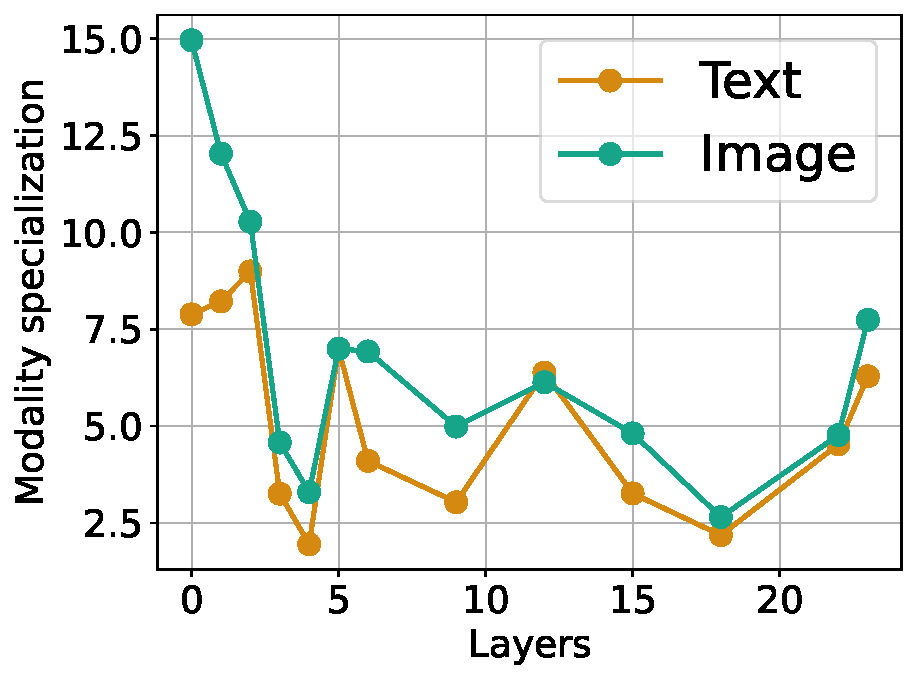
\includegraphics[width=1.0\textwidth]{assets/moes/specialization/model1088/modality_specialization_1088_150_across_layers.pdf}
        \end{subfigure}
        
        \caption{\textbf{Modality-specific specialization.} We visualize the experts specialization to text and image modalities. Models are evaluated on Obelics.}
        \label{fig:app_moes_specialization}
\end{wrapfigure}   



\subsection{Scaling laws evaluation and sensitivity}

For each model size and number of training tokens, we compute the loss based on the estimated functional form in \Cref{eq:scaling_laws} and compare it with the actual loss achieved by our runs. We visualize these points in \Cref{fig:observed_vs_predicted_loss}, demonstrating that our estimation is highly accurate, particularly for lower loss values, and hence for larger FLOPs. Additionally, we perform a sensitivity analysis using bootstrapping. Specifically, we sample with replacement \( P \) points (\( P \) being equal to the total number of trained models) and re-estimate the scaling law coefficients. This process is repeated 100 times, and we report the average and standard deviation of each coefficient. \Cref{tab:scaling_laws_sensitivity} shows that our estimation is more precise for \(\beta\) compared to \(\alpha\), primarily due to the smaller number of model sizes relative to the number of different token counts used to derive the scaling laws.  





\begin{table}[htb]
    \centering
    \setlength{\tabcolsep}{16pt} %
    \renewcommand{\arraystretch}{1} %
    \resizebox{0.9\linewidth}{!}{
    \begin{tabular}{lcccccccc}
        Model & E & $\alpha$ & $\beta$ & a & b  & d\\
        \midrule
        Avg  & 1.80922 & 0.29842 & 0.33209 & 0.54302  & 0.48301 &  0.92375 \\
        Std & 0.33811 & 0.10101 & 0.02892 & 0.08813 & 0.05787 & 0.23296 \\
        \bottomrule
    \end{tabular}%
    }
    \caption{\textbf{Scaling laws sensitivity.} We report the mean and standard deviation after bootstrapping with 100 iterations.}
    \label{tab:scaling_laws_sensitivity}
\end{table}


\subsection{\edit{Scaling laws for sparse NMMs.}}
\label{app:scaling_laws_moes}

Similar to dense models, we fit a parametric loss function (\Cref{eq:scaling_laws}) to predict the loss of sparse NMMs based on the number of parameters and training tokens, replacing the total parameter count with the number of active parameters. While incorporating sparsity is standard when deriving scaling laws for MoEs \citep{wangscalingmoe,krajewski2024scalingmoe,abnar2025parameters}, we focus on deriving scaling laws specific to the sparsity level used in our MoE setup. This yields coefficients that are implicitly conditioned on the sparsity configuration. 

We also experiment with a sparsity-aware formulation of the scaling law as proposed in \citep{abnar2025parameters}, and observe consistent trends (\Cref{tab:moes_coeffs}). In particular, the exponents associated with model size ($N$) are substantially larger than those for training tokens ($\beta$), reinforcing the importance of scaling model size in sparse architectures. Additionally, we observe that the terms governing the scaling of active parameters decompose into two components.


\begin{table}[h!]
    \begin{minipage}[b]{1\linewidth}
        \centering
        \setlength{\tabcolsep}{24pt}
        \renewcommand{\arraystretch}{1}
        \resizebox{1\linewidth}{!}{
        \begin{tabular}{ccc}
             \grayrow $L(N, D) = E+\frac{A}{N^{\alpha}}+\frac{B}{D^{\beta}}$ &vs&  $L(N, D, S) = \frac{A}{N^\alpha} + \frac{B}{D^\beta} + \frac{C}{(1 - S)^\lambda} + \frac{d}{(1 - S)^\delta N^\gamma} + E$ \\
        \end{tabular}
        }
      \label{tab:power_laws}
    \end{minipage}
    \begin{minipage}[b]{1\linewidth}
        \centering
        \setlength{\tabcolsep}{8pt}
        \renewcommand{\arraystretch}{1.1}
        \resizebox{1\linewidth}{!}{
        \begin{tabular}{lcccccccccc}
            Model & E & A & B & $\alpha$ & $\beta$ & $\lambda$ & $\delta$  & $\gamma$ & C & d  \\ %
            \shline
            
            $L(N, D)$ \Cref{eq:scaling_laws} & 2.158  & 381773 & 4659 & 0.710 & 0.372 & --  & -- & -- & -- & -- \\%& 46.19\\
            $L(N, D, S)$ \citep{abnar2025parameters} &  1.0788 & 1 & 4660 & 0.5890 & 0.3720 & 0.2 & 0.2 & 0.70956 & 1.0788 & 381475
        \end{tabular}%
        } 
        \caption{\textbf{Scaling laws for sparse native multimodal models}. Higher exponent for active parameters.}
        \label{tab:moes_coeffs}
    \end{minipage}    
\end{table}



\section{Mixture of experts and modality-specific specialization}
\label{app:moes}





We investigate multimodal specialization in MoE architectures. We compute a
specialization score as the average difference between the number of text/images
tokens assigned to each expert and a uniform assignment ($1/E$). Additionally,
we visualize the normalized number of text and image tokens assigned to each
expert across layers. \Cref{fig:app_moes_specialization} shows clear modality-specific
experts, particularly in the early layers. Furthermore, the specialization score
decreases as the number of layers increases but rises again in the very last
layers. This suggests that early and final layers require more modality
specialization compared to mid-layers. Additionally, we observe several experts
shared between text and image modalities, a phenomenon not present in
hard-routed or predefined modality-specific experts.


        



\begin{figure*}[h!]
    \centering
    \captionsetup{type=figure}
    \begin{subfigure}[t]{0.32\linewidth}
        \begin{tikzpicture}
    \begin{axis}[
        grid=both,
        grid style={line width=.1pt, draw=gray!10},
        major grid style={line width=.2pt,draw=gray!50},
        minor tick num=2,
        axis x line*=bottom,
        axis y line*=left,
        xmode=log, %
        log basis x=10, %
        xtick={
            1E+19,
            1E+20,
            1E+21,
            1E+22
        },
        xmin=2E+18,
        xmax=2E+22,
        ymax=4.5,
        width=1.15\linewidth,
        ylabel style={align=center, font=\scriptsize, yshift=-1ex},
        xlabel style={font=\scriptsize},
        ylabel={Validation Loss},
        xlabel={\scriptsize{FLOPs}},
        yticklabel style={font=\scriptsize},
        xticklabel style={font=\scriptsize},
        legend style={cells={align=left}, font=\scriptsize, fill opacity=0.7, fill=none,at={(0.1,0.95)}, anchor=west, draw=none}, %
        legend cell align={left},
        mark options={solid},
    ]



    \addplot[color=black, thick, samples=50, domain=5e18:10e21] {29.923*x^(-0.04936)};
    \addlegendentry{$L =  29.923C^{-0.0494}$};


    
    



    \addplot[legend late_0_2b style] plot coordinates {
        (4.03e+18, 4.017)
        (8.06e+18, 3.6149999999999998)
        (1.21e+19, 3.478)
        (2.02e+19, 3.3810000000000002)
        (4.03e+19, 3.23)
        (6.05e+19, 3.177)
        (8.06e+19, 3.1430000000000002)
        (1.61e+20, 3.066333333333333)
        (3.22e+20, 3.003666666666667)
        (4.84e+20, 2.969)
        (6.45e+20, 2.949)
    }; 
    \addplot[legend late_0_4b style] plot coordinates {
        (6.82e+18, 3.909333333333333)
        (1.36e+19, 3.5246666666666666)
        (2.04e+19, 3.388666666666667)
        (3.41e+19, 3.283666666666667)
        (6.82e+19, 3.1366666666666667)
        (1.02e+20, 3.078)
        (1.36e+20, 3.0436666666666667)
        (2.73e+20, 2.9633333333333334)
        (5.45e+20, 2.8993333333333333)
        (8.18e+20, 2.8653333333333335)
        (1.09e+21, 2.8433333333333333)
        (1.36e+21, 2.8256666666666668)
        (1.64e+21, 2.8156666666666665)
    };
    \addplot[legend late_0_9b style] plot coordinates {
        (1.38e+19, 3.9843333333333333)
        (2.77e+19, 3.4843333333333333)
        (4.15e+19, 3.324333333333333)
        (6.91e+19, 3.218)
        (1.38e+20, 3.032)
        (2.07e+20, 2.9636666666666667)
        (2.77e+20, 2.922333333333333)
        (5.53e+20, 2.828333333333333)
        (1.11e+21, 2.752666666666667)
        (1.66e+21, 2.7143333333333337)
        (2.21e+21, 2.690666666666667)
        (2.77e+21, 2.671)
        (3.32e+21, 2.6566666666666667)
    };

    \addplot[legend late style] plot coordinates {
        (2.4e+19, 3.873666666666667)
        (4.8e+19, 3.405333333333333)
        (7.2e+19, 3.252333333333333)
        (1.2e+20, 3.1483333333333334)
        (2.4e+20, 2.9559999999999995)
        (3.6e+20, 2.882)
        (4.8e+20, 2.8363333333333336)
        (9.6e+20, 2.735666666666667)
        (1.92e+21, 2.6553333333333335)
        (2.88e+21, 2.615666666666667)
        (3.84e+21, 2.5909999999999997)
        (4.8e+21, 2.573)
        (5.76e+21, 2.5606666666666666)
    };

    \addplot[legend late_2_2b style] plot coordinates {
        (3.34e+19, 3.828)
        (6.68e+19, 3.375)
        (1e+20, 3.2213333333333334)
        (1.67e+20, 3.114333333333333)
        (3.34e+20, 2.924666666666667)
        (5.01e+20, 2.8480000000000003)
        (6.68e+20, 2.801666666666667)
        (1.34e+21, 2.699666666666667)
        (2.67e+21, 2.615666666666667)
        (4.01e+21, 2.5736666666666665)
        (5.35e+21, 2.5473333333333334)
        (6.68e+21, 2.528333333333333)
        (8.02e+21, 2.5156666666666667)
    };
    \addplot[legend late_3_3b style] plot coordinates {
        (5.07e+19, 3.7769999999999997)
        (1.01e+20, 3.3369999999999997)
        (1.52e+20, 3.1846666666666668)
        (2.53e+20, 3.076333333333333)
        (5.07e+20, 2.8859999999999997)
        (7.6e+20, 2.8066666666666666)
        (1.01e+21, 2.7590000000000003)
        (2.03e+21, 2.653)
        (4.05e+21, 2.566666666666667)
        (6.08e+21, 2.525333333333333)
        (8.11e+21, 2.496)
        (1.01e+22, 2.4756666666666667)
        (1.22e+22, 2.4619999999999997)
    };
    

    \end{axis}
\end{tikzpicture}
    \end{subfigure}
    \begin{subfigure}[t]{0.32\linewidth}
        \begin{tikzpicture}
    \begin{axis}[
        grid=both,
        grid style={line width=.1pt, draw=gray!10},
        major grid style={line width=.2pt,draw=gray!50},
        minor tick num=2,
        axis x line*=bottom,
        axis y line*=left,
        xmode=log, %
        log basis x=10, %
        xtick={
            1E+19,
            1E+20,
            1E+21,
            1E+22
        },
        xmin=2E+18,
        xmax=2E+22,
        ymax=4.3,
        height=1.7in,
        width=1.15\linewidth,
        ylabel style={align=center, font=\scriptsize, yshift=-1ex},
        xlabel style={font=\scriptsize},
        title={\footnotesize{\colorbox{blue!10}{45-45-10}}},
        ylabel={Validation Loss},
        xlabel={\scriptsize{FLOPs}},
        yticklabel style={font=\scriptsize},
        xticklabel style={font=\scriptsize},
        legend style={cells={align=left}, font=\scriptsize, fill opacity=0.7, fill=none,at={(-0.3,0.95)}, anchor=west, draw=none}, %
        legend cell align={left},
        mark options={solid},
    ]


    \addplot[color=white, samples=50, domain=5e18:10e21, mark=none] {29.574*x^(-0.04919)};
    \addlegendentry{\scalebox{0.9}{$L = 29.574C^{-0.0492}$}};
    \addplot[color=black, samples=50, domain=5e18:10e21, forget plot] {29.574*x^(-0.04919)};


    

    
    



    \addplot[legend early_0_2b style, mark size=1pt] plot coordinates {
        (4.13e+18, 3.9896666666666665)
        (8.25e+18, 3.5996666666666663)
        (1.24e+19, 3.468)
        (2.06e+19, 3.358333333333333)
        (4.13e+19, 3.2113333333333336)
        (6.19e+19, 3.1543333333333337)
        (8.25e+19, 3.124)
        (1.65e+20, 3.048666666666667)
        (3.3e+20, 2.9836666666666667)
        (4.95e+20, 2.9506666666666668)
        (6.6e+20, 2.9309999999999996)
    };
    \addplot[legend early_0_4b style, mark size=1pt] plot coordinates {
        (6.96e+18, 3.887333333333333)
        (1.39e+19, 3.5203333333333333)
        (2.09e+19, 3.3823333333333334)
        (3.48e+19, 3.2710000000000004)
        (6.96e+19, 3.1170000000000004)
        (1.04e+20, 3.058666666666667)
        (1.39e+20, 3.0273333333333334)
        (2.78e+20, 2.9476666666666667)
        (5.57e+20, 2.877333333333333)
        (8.35e+20, 2.8433333333333333)
        (1.11e+21, 2.8223333333333334)
        (1.39e+21, 2.8063333333333333)
        (1.67e+21, 2.7936666666666667)
    };
    \addplot[legend early_0_9b style, mark size=1pt] plot coordinates {
        (1.4e+19, 3.955)
        (2.8e+19, 3.465)
        (4.19e+19, 3.3143333333333334)
        (6.99e+19, 3.2099999999999995)
        (1.4e+20, 3.0193333333333334)
        (2.1e+20, 2.9483333333333337)
        (2.8e+20, 2.9066666666666663)
        (5.59e+20, 2.807666666666666)
        (1.12e+21, 2.7273333333333327)
        (1.68e+21, 2.688333333333333)
        (2.24e+21, 2.666)
        (2.8e+21, 2.6466666666666665)
        (3.36e+21, 2.635333333333333)
    };

    \addplot[legend early style, mark size=1pt] plot coordinates {
        (2.44e+19, 3.859666666666667)
        (4.88e+19, 3.3973333333333335)
        (7.32e+19, 3.25)
        (1.22e+20, 3.1323333333333334)
        (2.44e+20, 2.9466666666666668)
        (3.66e+20, 2.875666666666667)
        (4.88e+20, 2.8206666666666664)
        (9.76e+20, 2.7246666666666672)
        (1.95e+21, 2.646666666666667)
        (2.93e+21, 2.6056666666666666)
        (3.9e+21, 2.582333333333333)
        (4.88e+21, 2.562)
        (5.86e+21, 2.548666666666666)
    };

    \addplot[legend early_2_2b style, mark size=1pt] plot coordinates {
        (3.42e+19, 3.859666666666667)
        (6.84e+19, 3.3973333333333335)
        (1.03e+20, 3.2503333333333333)
        (1.71e+20, 3.098333333333333)
        (3.42e+20, 2.9156666666666666)
        (5.13e+20, 2.8396666666666666)
        (6.84e+20, 2.7913333333333337)
        (1.37e+21, 2.687666666666667)
        (2.74e+21, 2.6026666666666665)
        (4.1e+21, 2.562)
        (5.47e+21, 2.5349999999999997)
        (6.84e+21, 2.5146666666666664)
        (8.21e+21, 2.502666666666667)
    };
    \addplot[legend early_3_3b style, mark size=1pt] plot coordinates {
        (5.03e+19, 3.746333333333333)
        (1.01e+20, 3.324)
        (1.51e+20, 3.1786666666666665)
        (2.52e+20, 3.0766666666666667)
        (5.03e+20, 2.8836666666666666)
        (7.55e+20, 2.8029999999999995)
        (1.01e+21, 2.7550000000000003)
        (2.01e+21, 2.6473333333333335)
        (4.02e+21, 2.5583333333333336)
        (6.04e+21, 2.5163333333333333)
        (8.05e+21, 2.4886666666666666)
        (1.01e+22, 2.466666666666667)
    };
    

    \end{axis}
\end{tikzpicture}
    \end{subfigure}
    \begin{subfigure}[t]{0.32\linewidth}
        \begin{tikzpicture}
    \begin{axis}[
        legend pos=north east,
        grid=both,
        grid style={line width=.1pt, draw=gray!10},
        major grid style={line width=.2pt,draw=gray!50},
        minor tick num=2,
        axis x line*=bottom,
        axis y line*=left,
        xmode=log, %
        log basis x=10, %
        xtick={
            1E+19,
            1E+20,
            1E+21,
            1E+22
        },
        xmin=2E+18,
        xmax=2E+22,
        ymax=4.5,
        width=1.15\linewidth,
        ylabel style={align=center, font=\scriptsize, yshift=-1ex},
        xlabel style={font=\scriptsize},
        ylabel={\scriptsize{Validation Loss}},
        xlabel={\scriptsize{FLOPs}},
        yticklabel style={font=\scriptsize},
        xticklabel style={font=\scriptsize},
        legend style={cells={align=left}, font=\scriptsize, fill opacity=0.7, fill=none, draw=none}, %
        mark options={solid},
    ]

        


    \addplot[color=black, thick, samples=50, domain=5e18:10e21] {26.287135104499598*x^(-0.04742807363789748)};
    \addlegendentry{$L = 26.287^{-0.047}$};



    
    



    \addplot[legend moe_0_2b style, mark size=1pt] plot coordinates {
        (4.13e+18, 4.182666666666666)
        (8.25e+18, 3.5933333333333333)
        (1.24e+19, 3.415333333333333)
        (2.06e+19, 3.2453333333333334)
        (4.13e+19, 3.098333333333333)
        (6.19e+19, 3.0340000000000003)
        (8.25e+19, 2.9949999999999997)
        (1.65e+20, 2.9066666666666663)
        (3.3e+20, 2.84)
        (4.95e+20, 2.798)
        (6.6e+20, 2.7773333333333334)
        (8.25e+20, 2.766666666666667)
        (9.9e+20, 2.7453333333333334)
        (1.16e+21, 2.736333333333333)
        (1.32e+21, 2.736666666666667)
    };
    \addplot[legend moe_0_4b style, mark size=1pt] plot coordinates {
        (6.96e+18, 4.010000000000001)
        (1.39e+19, 3.5096666666666665)
        (2.09e+19, 3.34)
        (3.48e+19, 3.173)
        (6.96e+19, 3.0226666666666664)
        (1.04e+20, 2.952666666666667)
        (1.39e+20, 2.899666666666667)
        (2.78e+20, 2.8106666666666666)
        (5.57e+20, 2.74)
        (8.35e+20, 2.7070000000000003)
        (1.11e+21, 2.6806666666666668)
        (1.39e+21, 2.6646666666666667)
        (1.67e+21, 2.651666666666667)
        (1.95e+21, 2.6460000000000004)
        (2.23e+21, 2.636)
    };
    \addplot[legend moe_0_9b style, mark size=1pt] plot coordinates {
        (1.4e+19, 4.270333333333333)
        (2.8e+19, 3.5366666666666666)
        (4.19e+19, 3.310333333333334)
        (6.99e+19, 3.112)
        (1.4e+20, 2.9346666666666663)
        (2.1e+20, 2.8510000000000004)
        (2.8e+20, 2.8073333333333337)
        (5.59e+20, 2.701333333333333)
        (1.12e+21, 2.6183333333333336)
        (1.68e+21, 2.5753333333333335)
        (2.24e+21, 2.5446666666666666)
        (2.8e+21, 2.5263333333333335)
        (3.36e+21, 2.514666666666667)
        (3.91e+21, 2.5003333333333333)
    };

    \addplot[legend moe style, mark size=1pt] plot coordinates {
        (2.44e+19, 4.198333333333333)
        (4.88e+19, 3.499333333333333)
        (7.32e+19, 3.2769999999999997)
        (1.22e+20, 3.0843333333333334)
        (2.44e+20, 2.8986666666666667)
        (3.66e+20, 2.8113333333333332)
        (4.88e+20, 2.764)
        (9.76e+20, 2.651333333333333)
        (1.95e+21, 2.5613333333333332)
        (2.93e+21, 2.5180000000000002)
        (3.9e+21, 2.5003333333333333)
        (4.88e+21, 2.4793333333333334)
        (5.86e+21, 2.4573333333333336)
        (6.83e+21, 2.4423333333333335)
        (7.81e+21, 2.4309999999999996)
    };

    \addplot[legend moe_2_2b style, mark size=1pt] plot coordinates {
        (3.42e+19, 4.194)
        (6.84e+19, 3.5239999999999996)
        (1.03e+20, 3.2906666666666666)
        (1.71e+20, 3.156333333333333)
        (3.42e+20, 2.9246666666666665)
        (5.13e+20, 2.821)
        (4.88e+20, 2.7543333333333333)
        (1.37e+21, 2.6296666666666666)
        (2.74e+21, 2.5369999999999995)
        (4.1e+21, 2.488)
        (5.47e+21, 2.458)
        (6.84e+21, 2.4436666666666667)
        (8.21e+21, 2.4246666666666665)
    };
    \addplot[legend moe_3_3b style, mark size=1pt] plot coordinates {
        (5.03e+19, 4.2043333333333335)
        (1.01e+20, 3.5156666666666667)
        (1.51e+20, 3.2786666666666666)
        (2.52e+20, 3.0673333333333335)
        (5.03e+20, 2.8800000000000003)
        (7.55e+20, 2.7840000000000003)
        (1.01e+21, 2.720333333333333)
        (2.01e+21, 2.613)
        (4.02e+21, 2.510333333333333)
        (6.04e+21, 2.46)
        (8.05e+21, 2.427)
        (1.01e+22, 2.40752)
        (1.21e+22, 2.3835766666666665)
    };
    

    \end{axis}
\end{tikzpicture}
    \end{subfigure}


    \makebox[0.9\linewidth]{ %
        \begin{tikzpicture}
            \begin{axis}[
                hide axis, %
                xmin=0, xmax=0.5, ymin=0, ymax=1, %
                legend columns=6, %
                legend style={
                    at={(0.5, 1)}, %
                    anchor=north, %
                    /tikz/every even column/.append style={column sep=0.2cm}, %
                    scale=0.5, %
                    cells={align=left}, font=\footnotesize,
                },
            ]

            \addlegendimage{legend late_0_2b style}
            \addlegendentry{0.289B}
            \addlegendimage{legend late_0_4b style}
            \addlegendentry{0.494B}
            \addlegendimage{legend late_0_9b style}
            \addlegendentry{1B}
            \addlegendimage{legend late style}
            \addlegendentry{1.748B}
            \addlegendimage{legend late_2_2b style}
            \addlegendentry{2.430B}
            \addlegendimage{legend late_3_3b style}
            \addlegendentry{3.714B}

            \addlegendimage{legend early_0_2b style}
            \addlegendentry{0.275B}
            \addlegendimage{legend early_0_4b style}
            \addlegendentry{0.464B}
            \addlegendimage{legend early_0_9b style}
            \addlegendentry{0.932B}
            \addlegendimage{legend early style}
            \addlegendentry{1.627B}
            \addlegendimage{legend early_2_2b style}
            \addlegendentry{2.280B}
            \addlegendimage{legend early_3_3b style}
            \addlegendentry{3.354B}

            \addlegendimage{legend moe_0_2b style}
            \addlegendentry{0.275B}
            \addlegendimage{legend moe_0_4b style}
            \addlegendentry{0.464B}
            \addlegendimage{legend moe_0_9b style}
            \addlegendentry{0.932B}
            \addlegendimage{legend moe style}
            \addlegendentry{1.627B}
            \addlegendimage{legend moe_2_2b style}
            \addlegendentry{2.280B}
            \addlegendimage{legend moe_3_3b style}
            \addlegendentry{3.354B}

            \end{axis}
        \end{tikzpicture}
    }

    \vspace{-4cm}

    \caption{\textbf{Scaling laws for native multimodal models.} From left to right: late-fusion (dense), early-fusion (dense) and early-fusion MoEs. The scaling exponents are very close for all models. However, MoEs leads to overall lower loss (smaller multiplicative constant) and takes longer to saturate.}
    \label{fig:scaling_laws_early_late_moe}
\end{figure*}



\begin{figure*}[h!]
    \centering
    \captionsetup{type=figure}

    \begin{subfigure}[t]{0.32\linewidth}
        
\begin{tikzpicture}
    \begin{axis}[
        legend pos=north east,
        grid=both,
        grid style={line width=.1pt, draw=gray!10},
        major grid style={line width=.2pt,draw=gray!50},
        minor tick num=2,
        axis x line*=bottom,
        axis y line*=left,
        xmode=log, %
        log basis x=10, %
        xtick={
            1E+19,
            1E+20,
            1E+21,
            1E+22
        },
        xmin=2E+18,
        xmax=2E+22,
        width=1.05\linewidth,
        ylabel style={align=center, font=\scriptsize, yshift=-1ex},
        xlabel style={font=\scriptsize},
        ylabel={\scriptsize{Image-Caption CE}},
        xlabel={\scriptsize{FLOPs}},
        yticklabel style={font=\scriptsize},
        xticklabel style={font=\scriptsize},
        legend style={cells={align=left}, font=\scriptsize, fill opacity=0.7, fill=none, draw=none}, %
        legend cell align={left},
        mark options={solid},
    ]



   \addplot[color=black, samples=50, domain=5e18:10e21] {49.99123471506872*x^(-0.061722162173828976)};
   \addlegendentry{$L = 49.99C^{-0.062}$};

    \addplot[legend late_0_2b style] plot coordinates {
        (4.05e+18, 4.006)
        (8.1e+18, 3.539)
        (1.21e+19, 3.373)
        (2.02e+19, 3.257)
        (4.05e+19, 3.067)
        (6.07e+19, 3.015)
        (8.1e+19, 2.967)
        (1.62e+20, 2.874)
        (3.24e+20, 2.797)
        (4.86e+20, 2.751)
        (6.48e+20, 2.728)
    };
    \addplot[legend late_0_4b style] plot coordinates {
        (6.85e+18, 3.903)
        (1.37e+19, 3.44)
        (2.05e+19, 3.273)
        (3.42e+19, 3.15)
        (6.85e+19, 2.975)
        (1.03e+20, 2.911)
        (1.37e+20, 2.869)
        (2.74e+20, 2.771)
        (5.48e+20, 2.695)
        (8.22e+20, 2.653)
        (1.1e+21, 2.626)
        (1.37e+21, 2.605)
        (1.64e+21, 2.593)
    };
    \addplot[legend late_0_9b style] plot coordinates {
        (1.39e+19, 3.988)
        (2.78e+19, 3.404)
        (4.17e+19, 3.215)
        (6.95e+19, 3.098)
        (1.39e+20, 2.859)
        (2.08e+20, 2.792)
        (2.78e+20, 2.734)
        (5.56e+20, 2.629)
        (1.11e+21, 2.541)
        (1.67e+21, 2.495)
        (2.22e+21, 2.467)
        (2.78e+21, 2.443)
        (3.34e+21, 2.422)
    };

    \addplot[legend late style] plot coordinates {
        (2.41e+19, 3.878)
        (4.82e+19, 3.32)
        (7.23e+19, 3.14)
        (1.21e+20, 3.03)
        (2.41e+20, 2.776)
        (3.62e+20, 2.696)
        (4.82e+20, 2.631)
        (9.65e+20, 2.513)
        (1.93e+21, 2.418)
        (2.89e+21, 2.373)
        (3.86e+21, 2.345)
        (4.82e+21, 2.322)
        (5.79e+21, 2.309)
    };
    \addplot[legend late_2_2b style] plot coordinates {
        (3.36e+19, 3.821)
        (6.72e+19, 3.284)
        (1.01e+20, 3.1)
        (1.68e+20, 2.98)
        (3.36e+20, 2.737)
        (5.04e+20, 2.651)
        (6.72e+20, 2.582)
        (1.34e+21, 2.466)
        (2.69e+21, 2.367)
        (4.03e+21, 2.319)
        (5.37e+21, 2.287)
        (6.72e+21, 2.267)
        (8.06e+21, 2.255)
    };
    \addplot[legend late_3_3b style] plot coordinates {
        (5.1e+19, 3.77)
        (1.02e+20, 3.244)
        (1.53e+20, 3.06)
        (2.55e+20, 2.943)
        (5.1e+20, 2.698)
        (7.64e+20, 2.607)
        (1.02e+21, 2.54)
        (2.04e+21, 2.416)
        (4.08e+21, 2.319)
        (6.11e+21, 2.268)
        (8.15e+21, 2.235)
        (1.02e+22, 2.21)
        (1.22e+22, 2.199)
    };
    

    \end{axis}
\end{tikzpicture}
    \end{subfigure}
    \begin{subfigure}[t]{0.32\linewidth}
        



\begin{tikzpicture}
    \begin{axis}[
        legend pos=north east,
        grid=both,
        grid style={line width=.1pt, draw=gray!10},
        major grid style={line width=.2pt,draw=gray!50},
        minor tick num=2,
        axis x line*=bottom,
        axis y line*=left,
        xmode=log, %
        log basis x=10, %
        xtick={
            1E+19,
            1E+20,
            1E+21,
            1E+22
        },
        xmin=2E+18,
        xmax=2E+22,
        width=1.05\linewidth,
        ylabel style={align=center, font=\scriptsize, yshift=-1ex},
        xlabel style={font=\scriptsize},
        ylabel={\scriptsize{Interleaved CE}},
        title={\footnotesize{\colorbox{blue!20}{45-45-10}}},
        xlabel={\scriptsize{FLOPs}},
        yticklabel style={font=\scriptsize},
        xticklabel style={font=\scriptsize},
        legend style={cells={align=left}, font=\scriptsize, fill opacity=0.7, fill=none, draw=none}, %
        legend cell align={left},
        mark options={solid},
    ]


    \addplot[color=black, samples=50, domain=5e18:10e21] {25.30255361628481*x^(-0.0459518153231069)};
    \addlegendentry{$L = 25.303^{-0.0460}$};

    \addplot[legend late_0_2b style] plot coordinates {
        (4.05e+18, 3.913)
        (8.1e+18, 3.538)
        (1.21e+19, 3.415)
        (2.02e+19, 3.326)
        (4.05e+19, 3.194)
        (6.07e+19, 3.14)
        (8.1e+19, 3.113)
        (1.62e+20, 3.044)
        (3.24e+20, 2.988)
        (4.86e+20, 2.959)
        (6.48e+20, 2.94)
    };
    \addplot[legend late_0_4b style] plot coordinates {
        (6.85e+18, 3.802)
        (1.37e+19, 3.451)
        (2.05e+19, 3.33)
        (3.42e+19, 3.234)
        (6.85e+19, 3.1)
        (1.03e+20, 3.043)
        (1.37e+20, 3.013)
        (2.74e+20, 2.942)
        (5.48e+20, 2.883)
        (8.22e+20, 2.853)
        (1.1e+21, 2.833)
        (1.37e+21, 2.815)
        (1.64e+21, 2.807)
    };
    \addplot[legend late_0_9b style] plot coordinates {
        (1.39e+19, 3.875)
        (2.78e+19, 3.409)
        (4.17e+19, 3.263)
        (6.95e+19, 3.161)
        (1.39e+20, 3.001)
        (2.08e+20, 2.931)
        (2.78e+20, 2.899)
        (5.56e+20, 2.811)
        (1.11e+21, 2.741)
        (1.67e+21, 2.707)
        (2.22e+21, 2.685)
        (2.78e+21, 2.666)
        (3.34e+21, 2.656)
    };

    \addplot[legend late style] plot coordinates {
        (2.41e+19, 3.764)
        (4.82e+19, 3.332)
        (7.23e+19, 3.192)
        (1.21e+20, 3.09)
        (2.41e+20, 2.929)
        (3.62e+20, 2.857)
        (4.82e+20, 2.822)
        (9.65e+20, 2.729)
        (1.93e+21, 2.656)
        (2.89e+21, 2.617)
        (3.86e+21, 2.594)
        (4.82e+21, 2.579)
        (5.79e+21, 2.568)
    };

    \addplot[legend late_2_2b style] plot coordinates {
        (3.36e+19, 3.722)
        (6.72e+19, 3.303)
        (1.01e+20, 3.164)
        (1.68e+20, 3.063)
        (3.36e+20, 2.9)
        (5.04e+20, 2.828)
        (6.72e+20, 2.793)
        (1.34e+21, 2.697)
        (2.69e+21, 2.621)
        (4.03e+21, 2.58)
        (5.37e+21, 2.557)
        (6.72e+21, 2.538)
        (8.06e+21, 2.527)
    };
    \addplot[legend late_3_3b style] plot coordinates {
        (5.1e+19, 3.67)
        (1.02e+20, 3.266)
        (1.53e+20, 3.129)
        (2.55e+20, 3.025)
        (5.1e+20, 2.862)
        (7.64e+20, 2.788)
        (1.02e+21, 2.75)
        (2.04e+21, 2.652)
        (4.08e+21, 2.568)
        (6.11e+21, 2.535)
        (8.15e+21, 2.506)
        (1.02e+22, 2.487)
        (1.22e+22, 2.472)
    };
    

    \end{axis}
\end{tikzpicture}
    \end{subfigure}
    \begin{subfigure}[t]{0.32\linewidth}
        
\begin{tikzpicture}
    \begin{axis}[
        legend pos=north east,
        grid=both,
        grid style={line width=.1pt, draw=gray!10},
        major grid style={line width=.2pt,draw=gray!50},
        minor tick num=2,
        axis x line*=bottom,
        axis y line*=left,
        xmode=log, %
        log basis x=10, %
        xtick={
            1E+19,
            1E+20,
            1E+21,
            1E+22
        },
        xmin=2E+18,
        xmax=2E+22,
        width=1.05\linewidth,
        ylabel style={align=center, font=\scriptsize, yshift=-1ex},
        xlabel style={font=\scriptsize},
        ylabel={\scriptsize{Text CE}},
        xlabel={\scriptsize{FLOPs}},
        yticklabel style={font=\scriptsize},
        xticklabel style={font=\scriptsize},
        legend style={cells={align=left}, font=\scriptsize, fill opacity=0.7, fill=none, draw=none}, %
        legend cell align={left},
        mark options={solid},
    ]


    \addplot[color=black, samples=50, domain=5e18:10e21] {22.64203*x^(-0.04193)};
    \addlegendentry{$L = 22.642^{-0.042}$};

    \addplot[legend late_0_2b style] plot coordinates {
        (4.05e+18, 4.132)
        (8.1e+18, 3.768)
        (1.21e+19, 3.646)
        (2.02e+19, 3.56)
        (4.05e+19, 3.429)
        (6.07e+19, 3.376)
        (8.1e+19, 3.349)
        (1.62e+20, 3.281)
        (3.24e+20, 3.226)
        (4.86e+20, 3.197)
        (6.48e+20, 3.179)
    };
    \addplot[legend late_0_4b style] plot coordinates {
        (6.85e+18, 4.023)
        (1.37e+19, 3.683)
        (2.05e+19, 3.563)
        (3.42e+19, 3.467)
        (6.85e+19, 3.335)
        (1.03e+20, 3.28)
        (1.37e+20, 3.249)
        (2.74e+20, 3.177)
        (5.48e+20, 3.12)
        (8.22e+20, 3.09)
        (1.1e+21, 3.071)
        (1.37e+21, 3.057)
        (1.64e+21, 3.047)
          
    };
    \addplot[legend late_0_9b style] plot coordinates {
        (1.39e+19, 4.09)
        (2.78e+19, 3.64)
        (4.17e+19, 3.495)
        (6.95e+19, 3.395)
        (1.39e+20, 3.236)
        (2.08e+20, 3.168)
        (2.78e+20, 3.134)
        (5.56e+20, 3.045)
        (1.11e+21, 2.976)
        (1.67e+21, 2.941)
        (2.22e+21, 2.92)
        (2.78e+21, 2.904)
        (3.34e+21, 2.892)
    };

    \addplot[legend late style] plot coordinates {
        (2.41e+19, 3.979)
        (4.82e+19, 3.564)
        (7.23e+19, 3.425)
        (1.21e+20, 3.325)
        (2.41e+20, 3.163)
        (3.62e+20, 3.093)
        (4.82e+20, 3.056)
        (9.65e+20, 2.965)
        (1.93e+21, 2.892)
        (2.89e+21, 2.857)
        (3.86e+21, 2.834)
        (4.82e+21, 2.818)
        (5.79e+21, 2.805)
    };

    \addplot[legend late_2_2b style] plot coordinates {
        (3.36e+19, 3.941)
        (6.72e+19, 3.538)
        (1.01e+20, 3.4)
        (1.68e+20, 3.3)
        (3.36e+20, 3.137)
        (5.04e+20, 3.065)
        (6.72e+20, 3.03)
        (1.34e+21, 2.936)
        (2.69e+21, 2.859)
        (4.03e+21, 2.822)
        (5.37e+21, 2.798)
        (6.72e+21, 2.78)
        (8.06e+21, 2.765)
    };
    \addplot[legend late_3_3b style] plot coordinates {
        (5.1e+19, 3.891)
        (1.02e+20, 3.501)
        (1.53e+20, 3.365)
        (2.55e+20, 3.261)
        (5.1e+20, 3.098)
        (7.64e+20, 3.025)
        (1.02e+21, 2.987)
        (2.04e+21, 2.891)
        (4.08e+21, 2.813)
        (6.11e+21, 2.773)
        (8.15e+21, 2.747)
        (1.02e+22, 2.73)
        (1.22e+22, 2.715)
    };
    

    \end{axis}
\end{tikzpicture}
    \end{subfigure}

    \begin{subfigure}[t]{0.32\linewidth}
        
\begin{tikzpicture}
    \begin{axis}[
        legend pos=north east,
        grid=both,
        grid style={line width=.1pt, draw=gray!10},
        major grid style={line width=.2pt,draw=gray!50},
        minor tick num=2,
        axis x line*=bottom,
        axis y line*=left,
        xmode=log, %
        log basis x=10, %
        xtick={
            1E+19,
            1E+20,
            1E+21,
            1E+22
        },
        xmin=2E+18,
        xmax=2E+22,
        width=1.05\linewidth,
        ylabel style={align=center, font=\scriptsize, yshift=-1ex},
        xlabel style={font=\scriptsize},
        ylabel={\scriptsize{Image-Caption CE}},
        xlabel={\scriptsize{FLOPs}},
        yticklabel style={font=\scriptsize},
        xticklabel style={font=\scriptsize},
        legend style={cells={align=left}, font=\scriptsize, fill opacity=0.7, fill=none, draw=none}, %
        legend cell align={left},
        mark options={solid},
    ]






    
    

   \addplot[color=black, samples=50, domain=5e18:10e21] {47.97*x^(-0.061)};
   \addlegendentry{$L = 47.97C^{-0.061}$};

    \addplot[legend early_0_2b style] plot coordinates {
        (4.13e+18, 3.969)
        (8.25e+18, 3.52)
        (1.24e+19, 3.366)
        (2.06e+19, 3.228)
        (4.13e+19, 3.048)
        (6.19e+19, 2.986)
        (8.25e+19, 2.95)
        (1.65e+20, 2.865)
        (3.3e+20, 2.781)
        (4.95e+20, 2.738)
        (6.6e+20, 2.715)  
    };
    \addplot[legend early_0_4b style] plot coordinates {
        (6.96e+18, 3.876)
        (1.39e+19, 3.451)
        (2.09e+19, 3.281)
        (3.48e+19, 3.145)
        (6.96e+19, 2.948)
        (1.04e+20, 2.886)
        (1.39e+20, 2.852)
        (2.78e+20, 2.755)
        (5.57e+20, 2.663)
        (8.35e+20, 2.621)
        (1.11e+21, 2.596)
        (1.39e+21, 2.579)
        (1.67e+21, 2.562)
    };
    \addplot[legend early_0_9b style] plot coordinates {
        (1.4e+19, 3.948)
        (2.8e+19, 3.375)
        (4.19e+19, 3.207)
        (6.99e+19, 3.096)
        (1.4e+20, 2.846)
        (2.1e+20, 2.772)
        (2.8e+20, 2.716)
        (5.59e+20, 2.598)
        (1.12e+21, 2.495)
        (1.68e+21, 2.448)
        (2.24e+21, 2.425)
        (2.8e+21, 2.401)
        (3.36e+21, 2.389)
    };

    \addplot[legend early style] plot coordinates {
        (2.44e+19, 3.842)
        (4.88e+19, 3.303)
        (7.32e+19, 3.141)
        (1.22e+20, 2.994)
        (2.44e+20, 2.761)
        (3.66e+20, 2.693)
        (4.88e+20, 2.606)
        (9.76e+20, 2.499)
        (1.95e+21, 2.409)
        (2.93e+21, 2.359)
        (3.9e+21, 2.334)
        (4.88e+21, 2.311)
        (5.86e+21, 2.299)
    };
    \addplot[legend early_2_2b style] plot coordinates {
        (3.42e+19, 3.842)
        (6.84e+19, 3.303)
        (1.03e+20, 3.142)
        (1.71e+20, 2.95)
        (3.42e+20, 2.729)
        (5.13e+20, 2.646)
        (6.84e+20, 2.576)
        (1.37e+21, 2.455)
        (2.74e+21, 2.352)
        (4.1e+21, 2.306)
        (5.47e+21, 2.279)
        (6.84e+21, 2.252)
        (8.21e+21, 2.242)
    };
    \addplot[legend early_3_3b style] plot coordinates {
        (5.03e+19, 3.719)
        (1.01e+20, 3.219)
        (1.51e+20, 3.051)
        (2.52e+20, 2.95)
        (5.03e+20, 2.7)
        (7.55e+20, 2.606)
        (1.01e+21, 2.543)
        (2.01e+21, 2.416)
        (4.02e+21, 2.307)
        (6.04e+21, 2.263)
        (8.05e+21, 2.232)
        (1.01e+22, 2.204)
        (1.21e+22, 2.197)
    };
    

    \end{axis}
\end{tikzpicture}
    \end{subfigure}
    \begin{subfigure}[t]{0.32\linewidth}
        



\begin{tikzpicture}
    \begin{axis}[
        legend pos=north east,
        grid=both,
        grid style={line width=.1pt, draw=gray!10},
        major grid style={line width=.2pt,draw=gray!50},
        minor tick num=2,
        axis x line*=bottom,
        axis y line*=left,
        xmode=log, %
        log basis x=10, %
        xtick={
            1E+19,
            1E+20,
            1E+21,
            1E+22
        },
        xmin=2E+18,
        xmax=2E+22,
        width=1.05\linewidth,
        ylabel style={align=center, font=\scriptsize, yshift=-1ex},
        title={\footnotesize{\colorbox{blue!20}{45-45-10}}},
        xlabel style={font=\scriptsize},
        ylabel={\scriptsize{Interleaved CE}},
        xlabel={\scriptsize{FLOPs}},
        yticklabel style={font=\scriptsize},
        xticklabel style={font=\scriptsize},
        legend style={cells={align=left}, font=\scriptsize, fill opacity=0.7, fill=none, draw=none}, %
        legend cell align={left},
        mark options={solid},
    ]






    
    

    \addplot[color=black, samples=50, domain=5e18:10e21] {25.114*x^(-0.0458)};
    \addlegendentry{$L = 25.114C^{-0.0458}$};

    \addplot[legend early_0_2b style] plot coordinates {
        (4.13e+18, 3.89)
        (8.25e+18, 3.524)
        (1.24e+19, 3.403)
        (2.06e+19, 3.306)
        (4.13e+19, 3.175)
        (6.19e+19, 3.12)
        (8.25e+19, 3.094)
        (1.65e+20, 3.022)
        (3.3e+20, 2.967)
        (4.95e+20, 2.939)
        (6.6e+20, 2.921)
    };
    \addplot[legend early_0_4b style] plot coordinates {
        (6.96e+18, 3.783)
        (1.39e+19, 3.44)
        (2.09e+19, 3.318)
        (3.48e+19, 3.217)
        (6.96e+19, 3.084)
        (1.04e+20, 3.027)
        (1.39e+20, 2.998)
        (2.78e+20, 2.927)
        (5.57e+20, 2.866)
        (8.35e+20, 2.836)
        (1.11e+21, 2.817)
        (1.39e+21, 2.8)
        (1.67e+21, 2.791)
    };
    \addplot[legend early_0_9b style] plot coordinates {
        (1.4e+19, 3.85)
        (2.8e+19, 3.394)
        (4.19e+19, 3.252)
        (6.99e+19, 3.15)
        (1.4e+20, 2.989)
        (2.1e+20, 2.919)
        (2.8e+20, 2.885)
        (5.59e+20, 2.795)
        (1.12e+21, 2.726)
        (1.68e+21, 2.691)
        (2.24e+21, 2.669)
        (2.8e+21, 2.651)
        (3.36e+21, 2.641)
    };

    \addplot[legend early style] plot coordinates {
        (2.44e+19, 3.759)
        (4.88e+19, 3.328)
        (7.32e+19, 3.188)
        (1.22e+20, 3.084)
        (2.44e+20, 2.922)
        (3.66e+20, 2.849)
        (4.88e+20, 2.811)
        (9.76e+20, 2.72)
        (1.95e+21, 2.648)
        (2.93e+21, 2.612)
        (3.9e+21, 2.59)
        (4.88e+21, 2.569)
        (5.86e+21, 2.554)
    };

    \addplot[legend early_2_2b style] plot coordinates {
        (3.42e+19, 3.759)
        (6.84e+19, 3.328)
        (1.03e+20, 3.188)
        (1.71e+20, 3.054)
        (3.42e+20, 2.891)
        (5.13e+20, 2.818)
        (6.84e+20, 2.781)
        (1.37e+21, 2.685)
        (2.74e+21, 2.61)
        (4.1e+21, 2.572)
        (5.47e+21, 2.542)
        (6.84e+21, 2.525)
        (8.21e+21, 2.514)
    };
    \addplot[legend early_3_3b style] plot coordinates {
        (5.03e+19, 3.649)
        (1.01e+20, 3.259)
        (1.51e+20, 3.125)
        (2.52e+20, 3.022)
        (5.03e+20, 2.858)
        (7.55e+20, 2.784)
        (1.01e+21, 2.744)
        (2.01e+21, 2.645)
        (4.02e+21, 2.566)
        (6.04e+21, 2.523)
        (8.05e+21, 2.497)
        (1.01e+22, 2.477)
        (1.21e+22, 2.467)
    };
    

    \end{axis}
\end{tikzpicture}
    \end{subfigure}
    \begin{subfigure}[t]{0.32\linewidth}
        
\begin{tikzpicture}
    \begin{axis}[
        legend pos=north east,
        grid=both,
        grid style={line width=.1pt, draw=gray!10},
        major grid style={line width=.2pt,draw=gray!50},
        minor tick num=2,
        axis x line*=bottom,
        axis y line*=left,
        xmode=log, %
        log basis x=10, %
        xtick={
            1E+19,
            1E+20,
            1E+21,
            1E+22
        },
        xmin=2E+18,
        xmax=2E+22,
        width=1.05\linewidth,
        ylabel style={align=center, font=\scriptsize, yshift=-1ex},
        xlabel style={font=\scriptsize},
        ylabel={\scriptsize{Text CE}},
        xlabel={\scriptsize{FLOPs}},
        yticklabel style={font=\scriptsize},
        xticklabel style={font=\scriptsize},
        legend style={cells={align=left}, font=\scriptsize, fill opacity=0.7, fill=none, draw=none}, %
        legend cell align={left},
        mark options={solid},
    ]


    \addplot[color=black, samples=50, domain=5e18:10e21] {22.709*x^(-0.042)};
    \addlegendentry{$L = 22.709C^{-0.042}$};

    \addplot[legend early_0_2b style] plot coordinates {
        (4.13e+18, 4.11)
        (8.25e+18, 3.755)
        (1.24e+19, 3.635)
        (2.06e+19, 3.541)
        (4.13e+19, 3.411)
        (6.19e+19, 3.357)
        (8.25e+19, 3.328)
        (1.65e+20, 3.259)
        (3.3e+20, 3.203)
        (4.95e+20, 3.175)
        (6.6e+20, 3.157)
    };
    \addplot[legend early_0_4b style] plot coordinates {
        (6.96e+18, 4.003)
        (1.39e+19, 3.67)
        (2.09e+19, 3.548)
        (3.48e+19, 3.451)
        (6.96e+19, 3.319)
        (1.04e+20, 3.263)
        (1.39e+20, 3.232)
        (2.78e+20, 3.161)
        (5.57e+20, 3.103)
        (8.35e+20, 3.073)
        (1.11e+21, 3.054)
        (1.39e+21, 3.04)
        (1.67e+21, 3.028)
        
          
    };
    \addplot[legend early_0_9b style] plot coordinates {
        (1.4e+19, 4.067)
        (2.8e+19, 3.626)
        (4.19e+19, 3.484)
        (6.99e+19, 3.384)
        (1.4e+20, 3.223)
        (2.1e+20, 3.154)
        (2.8e+20, 3.119)
        (5.59e+20, 3.03)
        (1.12e+21, 2.961)
        (1.68e+21, 2.926)
        (2.24e+21, 2.904)
        (2.8e+21, 2.888)
        (3.36e+21, 2.876)
    };

    \addplot[legend early style] plot coordinates {
        (2.44e+19, 3.978)
        (4.88e+19, 3.561)
        (7.32e+19, 3.421)
        (1.22e+20, 3.319)
        (2.44e+20, 3.157)
        (3.66e+20, 3.085)
        (4.88e+20, 3.045)
        (9.76e+20, 2.955)
        (1.95e+21, 2.883)
        (2.93e+21, 2.846)
        (3.9e+21, 2.823)
        (4.88e+21, 2.806)
        (5.86e+21, 2.793)
    };

    \addplot[legend early_2_2b style] plot coordinates {
        (3.42e+19, 3.978)
        (6.84e+19, 3.561)
        (1.03e+20, 3.421)
        (1.71e+20, 3.291)
        (3.42e+20, 3.127)
        (5.13e+20, 3.055)
        (6.84e+20, 3.017)
        (1.37e+21, 2.923)
        (2.74e+21, 2.846)
        (4.1e+21, 2.808)
        (5.47e+21, 2.784)
        (6.84e+21, 2.767)
        (8.21e+21, 2.752)
    };
    \addplot[legend early_3_3b style] plot coordinates {
        (5.03e+19, 3.871)
        (1.01e+20, 3.494)
        (1.51e+20, 3.36)
        (2.52e+20, 3.258)
        (5.03e+20, 3.093)
        (7.55e+20, 3.019)
        (1.01e+21, 2.978)
        (2.01e+21, 2.881)
        (4.02e+21, 2.802)
        (6.04e+21, 2.763)
        (8.05e+21, 2.737)
        (1.01e+22, 2.719)
        (1.21e+22, 2.704)
    };
    

    \end{axis}
\end{tikzpicture}
    \end{subfigure}


    \begin{subfigure}[t]{0.32\linewidth}
        
\begin{tikzpicture}
    \begin{axis}[
        legend pos=north east,
        grid=both,
        grid style={line width=.1pt, draw=gray!10},
        major grid style={line width=.2pt,draw=gray!50},
        minor tick num=2,
        axis x line*=bottom,
        axis y line*=left,
        xmode=log, %
        log basis x=10, %
        xtick={
            1E+19,
            1E+20,
            1E+21,
            1E+22
        },
        xmin=2E+18,
        xmax=2E+22,
        ymax=4.5,
        width=1.15\linewidth,
        ylabel style={align=center, font=\scriptsize, yshift=-1ex},
        xlabel style={font=\scriptsize},
        ylabel={\scriptsize{Image-Caption CE}},
        xlabel={\scriptsize{FLOPs}},
        yticklabel style={font=\scriptsize},
        xticklabel style={font=\scriptsize},
        legend style={cells={align=left}, font=\scriptsize, fill opacity=0.7, draw=none}, %
        legend cell align={left},
        mark options={solid},
    ]




    \addplot[color=black, thick, samples=50, domain=5e18:10e21] {70.64022825064674*x^(-0.07028124966310799)};
    \addlegendentry{$L = 70.64^{-0.0703}$};
 

    \addplot[legend moe_0_2b style] plot coordinates {
(4.13e+18, 4.188)
(8.25e+18, 3.496)
(1.24e+19, 3.287)
(2.06e+19, 3.095)
(4.13e+19, 2.935)
(6.19e+19, 2.865)
(8.25e+19, 2.809)
(1.65e+20, 2.702)
(3.3e+20, 2.628)
(4.95e+20, 2.568)
(6.6e+20, 2.551)
(8.25e+20, 2.547)
(9.9e+20, 2.508)
(1.16e+21, 2.477)
(1.32e+21, 2.491)
    };

    \addplot[legend moe_0_4b style] plot coordinates {
(6.96e+18, 4.009)
(1.39e+19, 3.408)
(2.09e+19, 3.212)
(3.48e+19, 3.029)
(6.96e+19, 2.866)
(1.04e+20, 2.782)
(1.39e+20, 2.697)
(2.78e+20, 2.591)
(5.57e+20, 2.507)
(8.35e+20, 2.472)
(1.11e+21, 2.439)
(1.39e+21, 2.421)
(1.67e+21, 2.408)
(1.95e+21, 2.387)
(2.23e+21, 2.373)
    };

    \addplot[legend moe_0_9b style] plot coordinates {
(1.4e+19, 4.257)
(2.8e+19, 3.431)
(4.19e+19, 3.166)
(6.99e+19, 2.943)
(1.4e+20, 2.748)
(2.1e+20, 2.646)
(2.8e+20, 2.586)
(5.59e+20, 2.462)
(1.12e+21, 2.37)
(1.68e+21, 2.317)
(2.24e+21, 2.289)
(2.8e+21, 2.262)
(3.36e+21, 2.256)
(3.91e+21, 2.213)
    };

    \addplot[legend moe style] plot coordinates {
(2.44e+19, 4.161)
(4.88e+19, 3.381)
(7.32e+19, 3.123)
(1.22e+20, 2.916)
(2.44e+20, 2.706)
(3.66e+20, 2.6)
(4.88e+20, 2.537)
(9.76e+20, 2.405)
(1.95e+21, 2.302)
(2.93e+21, 2.257)
(3.9e+21, 2.216)
(4.88e+21, 2.189)
(5.86e+21, 2.162)
(6.83e+21, 2.147)
(7.81e+21, 2.132)
    };




    \addplot[legend moe_2_2b style] plot coordinates {
(3.42e+19, 4.098)
(6.84e+19, 3.398)
(1.03e+20, 3.117)
(1.71e+20, 2.956)
(3.42e+20, 2.712)
(5.13e+20, 2.588)
(4.88e+20, 2.496)
(1.37e+21, 2.358)
(2.74e+21, 2.257)
(4.1e+21, 2.199)
(5.47e+21, 2.166)
(6.84e+21, 2.146)
(8.21e+21, 2.119)
    };
    \addplot[legend moe_3_3b style] plot coordinates {
(5.03e+19, 4.103)
(1.01e+20, 3.39)
(1.51e+20, 3.105)
(2.52e+20, 2.858)
(5.03e+20, 2.663)
(7.55e+20, 2.544)
(1.01e+21, 2.458)
(2.01e+21, 2.337)
(4.02e+21, 2.223)
(6.04e+21, 2.168)
(8.05e+21, 2.129)
(1.01e+22, 2.10901)
(1.21e+22, 2.07879)
    };


    \end{axis}
\end{tikzpicture}
    \end{subfigure}
    \begin{subfigure}[t]{0.32\linewidth}
        



\begin{tikzpicture}
    \begin{axis}[
        legend pos=north east,
        grid=both,
        grid style={line width=.1pt, draw=gray!10},
        major grid style={line width=.2pt,draw=gray!50},
        minor tick num=2,
        axis x line*=bottom,
        axis y line*=left,
        xmode=log, %
        log basis x=10, %
        xtick={
            1E+19,
            1E+20,
            1E+21,
            1E+22
        },
        xmin=2E+18,
        xmax=2E+22,
        ymax=4.5,
        width=1.15\linewidth,
        ylabel style={align=center, font=\scriptsize, yshift=-1ex},
        xlabel style={font=\scriptsize},
        title={\footnotesize{\colorbox{blue!20}{45-45-10}}},
        ylabel={\scriptsize{Interleaved CE}},
        xlabel={\scriptsize{FLOPs}},
        yticklabel style={font=\scriptsize},
        xticklabel style={font=\scriptsize},
        legend style={cells={align=left}, font=\scriptsize, fill opacity=0.7, draw=none}, %
        legend cell align={left},
        mark options={solid},
    ]

    \addplot[color=black, thick, samples=50, domain=5e18:10e21] {22.2376901700986*x^(-0.04386160285945637)};
    \addlegendentry{$L = 22.238^{-0.0439}$};
 
    \addplot[legend moe_0_2b style] plot coordinates {
(4.13e+18, 4.074)
(8.25e+18, 3.533)
(1.24e+19, 3.373)
(2.06e+19, 3.213)
(4.13e+19, 3.073)
(6.19e+19, 3.011)
(8.25e+19, 2.981)
(1.65e+20, 2.901)
(3.3e+20, 2.839)
(4.95e+20, 2.806)
(6.6e+20, 2.783)
(8.25e+20, 2.769)
(9.9e+20, 2.756)
(1.16e+21, 2.741)
(1.32e+21, 2.736)
    };

    \addplot[legend moe_0_4b style] plot coordinates {
(6.96e+18, 3.904)
(1.39e+19, 3.452)
(2.09e+19, 3.298)
(3.48e+19, 3.137)
(6.96e+19, 2.994)
(1.04e+20, 2.931)
(1.39e+20, 2.895)
(2.78e+20, 2.814)
(5.57e+20, 2.75)
(8.35e+20, 2.718)
(1.11e+21, 2.693)
(1.39e+21, 2.679)
(1.67e+21, 2.665)
(1.95e+21, 2.652)
(2.23e+21, 2.644) 
    };

    \addplot[legend moe_0_9b style] plot coordinates {
(1.4e+19, 4.165)
(2.8e+19, 3.481)
(4.19e+19, 3.275)
(6.99e+19, 3.089)
(1.4e+20, 2.921)
(2.1e+20, 2.846)
(2.8e+20, 2.812)
(5.59e+20, 2.714)
(1.12e+21, 2.636)
(1.68e+21, 2.597)
(2.24e+21, 2.559)
(2.8e+21, 2.55)
(3.36e+21, 2.536)
(3.91e+21, 2.521)
    };

    \addplot[legend moe style] plot coordinates {
(2.44e+19, 4.105)
(4.88e+19, 3.449)
(7.32e+19, 3.246)
(1.22e+20, 3.06)
(2.44e+20, 2.887)
(3.66e+20, 2.809)
(4.88e+20, 2.77)
(9.76e+20, 2.667)
(1.95e+21, 2.583)
(2.93e+21, 2.541)
(3.9e+21, 2.519)
(4.88e+21, 2.501)
(5.86e+21, 2.482)
(6.83e+21, 2.467)
(7.81e+21, 2.459)
    };

    \addplot[legend moe_2_2b style] plot coordinates {
(3.42e+19, 4.118)
(6.84e+19, 3.463)
(1.03e+20, 3.255)
(1.71e+20, 3.133)
(3.42e+20, 2.908)
(5.13e+20, 2.814)
(4.88e+20, 2.76)
(1.37e+21, 2.643)
(2.74e+21, 2.554)
(4.1e+21, 2.51)
(5.47e+21, 2.482)
(6.84e+21, 2.468)
(8.21e+21, 2.453)
    };
    \addplot[legend moe_3_3b style] plot coordinates {
(5.03e+19, 4.13)
(1.01e+20, 3.455)
(1.51e+20, 3.243)
(2.52e+20, 3.048)
(5.03e+20, 2.865)
(7.55e+20, 2.78)
(1.01e+21, 2.727)
(2.01e+21, 2.627)
(4.02e+21, 2.53)
(6.04e+21, 2.482)
(8.05e+21, 2.452)
(1.01e+22, 2.43128)
(1.21e+22, 2.41114)
    };




    \end{axis}
\end{tikzpicture}
    \end{subfigure}
    \begin{subfigure}[t]{0.32\linewidth}
        
\begin{tikzpicture}
    \begin{axis}[
        legend pos=north east,
        grid=both,
        grid style={line width=.1pt, draw=gray!10},
        major grid style={line width=.2pt,draw=gray!50},
        minor tick num=2,
        axis x line*=bottom,
        axis y line*=left,
        xmode=log, %
        log basis x=10, %
        xtick={
            1E+19,
            1E+20,
            1E+21,
            1E+22
        },
        xmin=2E+18,
        xmax=2E+22,
        ymax=4.5,
        width=1.15\linewidth,
        ylabel style={align=center, font=\scriptsize, yshift=-3ex},
        xlabel style={font=\scriptsize},
        ylabel={\scriptsize{Text CE}},
        xlabel={\scriptsize{FLOPs}},
        yticklabel style={font=\scriptsize},
        xticklabel style={font=\scriptsize},
        legend style={cells={align=left}, font=\scriptsize, fill opacity=0.7, draw=none}, %
        legend cell align={left},
        mark options={solid},
    ]

    

    

    


   
    

   \addplot[color=black, thick, samples=50, domain=5e18:10e21] {19.31783579322471*x^(-0.03928902115176261)};
   \addlegendentry{$L = 19.318C^{-0.0393}$};


    \addplot[legend moe_0_2b style] plot coordinates {
        (4.13e+18, 4.286)
        (8.25e+18, 3.751)
        (1.24e+19, 3.586)
        (2.06e+19, 3.428)
        (4.13e+19, 3.287)
        (6.19e+19, 3.226)
        (8.25e+19, 3.195)
        (1.65e+20, 3.117)
        (3.3e+20, 3.053)
        (4.95e+20, 3.02)
        (6.6e+20, 2.998)
        (8.25e+20, 2.984)
        (9.9e+20, 2.972)
        (1.16e+21, 2.991)
        (1.32e+21, 2.983)
    };

    \addplot[legend moe_0_4b style] plot coordinates {
        (6.96e+18, 4.117)
        (1.39e+19, 3.669)
        (2.09e+19, 3.51)
        (3.48e+19, 3.353)
        (6.96e+19, 3.208)
        (1.04e+20, 3.145)
        (1.39e+20, 3.107)
        (2.78e+20, 3.027)
        (5.57e+20, 2.963)
        (8.35e+20, 2.931)
        (1.11e+21, 2.91)
        (1.39e+21, 2.894)
        (1.67e+21, 2.882)
        (1.95e+21, 2.899)
        (2.23e+21, 2.891)
    };

    \addplot[legend moe_0_9b style] plot coordinates {
        (1.4e+19, 4.389)
        (2.8e+19, 3.698)
        (4.19e+19, 3.49)
        (6.99e+19, 3.304)
        (1.4e+20, 3.135)
        (2.1e+20, 3.061)
        (2.8e+20, 3.024)
        (5.59e+20, 2.928)
        (1.12e+21, 2.849)
        (1.68e+21, 2.812)
        (2.24e+21, 2.786)
        (2.8e+21, 2.767)
        (3.36e+21, 2.752)
        (3.91e+21, 2.767)
    };

    \addplot[legend moe style] plot coordinates {
        (2.44e+19, 4.329)
        (4.88e+19, 3.668)
        (7.32e+19, 3.462)
        (1.22e+20, 3.277)
        (2.44e+20, 3.103)
        (3.66e+20, 3.025)
        (4.88e+20, 2.985)
        (9.76e+20, 2.882)
        (1.95e+21, 2.799)
        (2.93e+21, 2.756)
        (3.9e+21, 2.766)
        (4.88e+21, 2.748)
        (5.86e+21, 2.728)
        (6.83e+21, 2.713)
        (7.81e+21, 2.702)
        
    };

    \addplot[legend moe_2_2b style] plot coordinates {
        (3.42e+19, 4.366)
        (6.84e+19, 3.711)
        (1.03e+20, 3.5)
        (1.71e+20, 3.38)
        (3.42e+20, 3.154)
        (5.13e+20, 3.061)
        (4.88e+20, 3.007)
        (1.37e+21, 2.888)
        (2.74e+21, 2.8)
        (4.1e+21, 2.755)
        (5.47e+21, 2.726)
        (6.84e+21, 2.717)
        (8.21e+21, 2.702)
    };
    \addplot[legend moe_3_3b style] plot coordinates {
        (5.03e+19, 4.38)
        (1.01e+20, 3.702)
        (1.51e+20, 3.488)
        (2.52e+20, 3.296)
        (5.03e+20, 3.112)
        (7.55e+20, 3.028)
        (1.01e+21, 2.976)
        (2.01e+21, 2.875)
        (4.02e+21, 2.778)
        (6.04e+21, 2.73)
        (8.05e+21, 2.7)
        (1.01e+22, 2.68227)
        (1.21e+22, 2.6608)
        
    };
    \end{axis}
\end{tikzpicture}
    \end{subfigure}


    \makebox[0.9\linewidth]{ %
        \begin{tikzpicture}
            \begin{axis}[
                hide axis, %
                xmin=0, xmax=0.5, ymin=0, ymax=1, %
                legend columns=6, %
                legend style={
                    at={(0.5, 1)}, %
                    anchor=north, %
                    /tikz/every even column/.append style={column sep=0.2cm}, %
                    scale=0.5, %
                    cells={align=left}, font=\footnotesize,
                },
            ]

            \addlegendimage{legend late_0_2b style}
            \addlegendentry{0.289B}
            \addlegendimage{legend late_0_4b style}
            \addlegendentry{0.494B}
            \addlegendimage{legend late_0_9b style}
            \addlegendentry{1B}
            \addlegendimage{legend late style}
            \addlegendentry{1.748B}
            \addlegendimage{legend late_2_2b style}
            \addlegendentry{2.430B}
            \addlegendimage{legend late_3_3b style}
            \addlegendentry{3.714B}

            \addlegendimage{legend early_0_2b style}
            \addlegendentry{0.275B}
            \addlegendimage{legend early_0_4b style}
            \addlegendentry{0.464B}
            \addlegendimage{legend early_0_9b style}
            \addlegendentry{0.932B}
            \addlegendimage{legend early style}
            \addlegendentry{1.627B}
            \addlegendimage{legend early_2_2b style}
            \addlegendentry{2.280B}
            \addlegendimage{legend early_3_3b style}
            \addlegendentry{3.354B}

            \addlegendimage{legend moe_0_2b style}
            \addlegendentry{0.275B}
            \addlegendimage{legend moe_0_4b style}
            \addlegendentry{0.464B}
            \addlegendimage{legend moe_0_9b style}
            \addlegendentry{0.932B}
            \addlegendimage{legend moe style}
            \addlegendentry{1.627B}
            \addlegendimage{legend moe_2_2b style}
            \addlegendentry{2.280B}
            \addlegendimage{legend moe_3_3b style}
            \addlegendentry{3.354B}

            \end{axis}
        \end{tikzpicture}
    }

    \vspace{-4cm}
    \caption{\textbf{Scaling laws for native multimodal models.} From top to bottom: late-fusion (dense), early-fusion (dense) and early-fusion MoEs. From left to right: cross-entropy on the validation set of image-caption, interleaved and text-only data.}
    \label{fig:scaling_laws_early_late_moe_getty_obelics_dclm}
\end{figure*}




























\begin{figure*}[h!]
    \centering
    \captionsetup{type=figure}
    \begin{subfigure}[t]{0.32\linewidth}
        
\begin{tikzpicture}
    \begin{axis}[
        legend pos=north east,
        grid=both,
        grid style={line width=.1pt, draw=gray!10},
        major grid style={line width=.2pt,draw=gray!50},
        minor tick num=2,
        axis x line*=bottom,
        axis y line*=left,
        xmode=log, %
        log basis x=10, %
        xtick={
            1E+19,
            1E+20,
            1E+21,
            1E+22
        },
        xmin=2E+18,
        xmax=2E+22,
        width=1.05\linewidth,
        ylabel style={align=center, font=\scriptsize, yshift=-1ex},
        xlabel style={font=\scriptsize},
        ylabel={\scriptsize{Image-Caption CE}},
        xlabel={\scriptsize{FLOPs}},
        yticklabel style={font=\scriptsize},
        xticklabel style={font=\scriptsize},
        legend style={cells={align=left}, font=\scriptsize, fill opacity=0.7, fill=none, draw=none}, %
        legend cell align={left},
        mark options={solid},
    ]






    
    

   \addplot[color=black, samples=50, domain=5e18:10e21] {47.97*x^(-0.061)};
   \addlegendentry{$L = 47.97C^{-0.061}$};

    \addplot[legend early_0_2b style] plot coordinates {
        (4.13e+18, 3.969)
        (8.25e+18, 3.52)
        (1.24e+19, 3.366)
        (2.06e+19, 3.228)
        (4.13e+19, 3.048)
        (6.19e+19, 2.986)
        (8.25e+19, 2.95)
        (1.65e+20, 2.865)
        (3.3e+20, 2.781)
        (4.95e+20, 2.738)
        (6.6e+20, 2.715)  
    };
    \addplot[legend early_0_4b style] plot coordinates {
        (6.96e+18, 3.876)
        (1.39e+19, 3.451)
        (2.09e+19, 3.281)
        (3.48e+19, 3.145)
        (6.96e+19, 2.948)
        (1.04e+20, 2.886)
        (1.39e+20, 2.852)
        (2.78e+20, 2.755)
        (5.57e+20, 2.663)
        (8.35e+20, 2.621)
        (1.11e+21, 2.596)
        (1.39e+21, 2.579)
        (1.67e+21, 2.562)
    };
    \addplot[legend early_0_9b style] plot coordinates {
        (1.4e+19, 3.948)
        (2.8e+19, 3.375)
        (4.19e+19, 3.207)
        (6.99e+19, 3.096)
        (1.4e+20, 2.846)
        (2.1e+20, 2.772)
        (2.8e+20, 2.716)
        (5.59e+20, 2.598)
        (1.12e+21, 2.495)
        (1.68e+21, 2.448)
        (2.24e+21, 2.425)
        (2.8e+21, 2.401)
        (3.36e+21, 2.389)
    };

    \addplot[legend early style] plot coordinates {
        (2.44e+19, 3.842)
        (4.88e+19, 3.303)
        (7.32e+19, 3.141)
        (1.22e+20, 2.994)
        (2.44e+20, 2.761)
        (3.66e+20, 2.693)
        (4.88e+20, 2.606)
        (9.76e+20, 2.499)
        (1.95e+21, 2.409)
        (2.93e+21, 2.359)
        (3.9e+21, 2.334)
        (4.88e+21, 2.311)
        (5.86e+21, 2.299)
    };
    \addplot[legend early_2_2b style] plot coordinates {
        (3.42e+19, 3.842)
        (6.84e+19, 3.303)
        (1.03e+20, 3.142)
        (1.71e+20, 2.95)
        (3.42e+20, 2.729)
        (5.13e+20, 2.646)
        (6.84e+20, 2.576)
        (1.37e+21, 2.455)
        (2.74e+21, 2.352)
        (4.1e+21, 2.306)
        (5.47e+21, 2.279)
        (6.84e+21, 2.252)
        (8.21e+21, 2.242)
    };
    \addplot[legend early_3_3b style] plot coordinates {
        (5.03e+19, 3.719)
        (1.01e+20, 3.219)
        (1.51e+20, 3.051)
        (2.52e+20, 2.95)
        (5.03e+20, 2.7)
        (7.55e+20, 2.606)
        (1.01e+21, 2.543)
        (2.01e+21, 2.416)
        (4.02e+21, 2.307)
        (6.04e+21, 2.263)
        (8.05e+21, 2.232)
        (1.01e+22, 2.204)
        (1.21e+22, 2.197)
    };
    

    \end{axis}
\end{tikzpicture}
    \end{subfigure}
    \begin{subfigure}[t]{0.32\linewidth}
        



\begin{tikzpicture}
    \begin{axis}[
        legend pos=north east,
        grid=both,
        grid style={line width=.1pt, draw=gray!10},
        major grid style={line width=.2pt,draw=gray!50},
        minor tick num=2,
        axis x line*=bottom,
        axis y line*=left,
        xmode=log, %
        log basis x=10, %
        xtick={
            1E+19,
            1E+20,
            1E+21,
            1E+22
        },
        xmin=2E+18,
        xmax=2E+22,
        width=1.05\linewidth,
        ylabel style={align=center, font=\scriptsize, yshift=-1ex},
        title={\footnotesize{\colorbox{blue!20}{45-45-10}}},
        xlabel style={font=\scriptsize},
        ylabel={\scriptsize{Interleaved CE}},
        xlabel={\scriptsize{FLOPs}},
        yticklabel style={font=\scriptsize},
        xticklabel style={font=\scriptsize},
        legend style={cells={align=left}, font=\scriptsize, fill opacity=0.7, fill=none, draw=none}, %
        legend cell align={left},
        mark options={solid},
    ]






    
    

    \addplot[color=black, samples=50, domain=5e18:10e21] {25.114*x^(-0.0458)};
    \addlegendentry{$L = 25.114C^{-0.0458}$};

    \addplot[legend early_0_2b style] plot coordinates {
        (4.13e+18, 3.89)
        (8.25e+18, 3.524)
        (1.24e+19, 3.403)
        (2.06e+19, 3.306)
        (4.13e+19, 3.175)
        (6.19e+19, 3.12)
        (8.25e+19, 3.094)
        (1.65e+20, 3.022)
        (3.3e+20, 2.967)
        (4.95e+20, 2.939)
        (6.6e+20, 2.921)
    };
    \addplot[legend early_0_4b style] plot coordinates {
        (6.96e+18, 3.783)
        (1.39e+19, 3.44)
        (2.09e+19, 3.318)
        (3.48e+19, 3.217)
        (6.96e+19, 3.084)
        (1.04e+20, 3.027)
        (1.39e+20, 2.998)
        (2.78e+20, 2.927)
        (5.57e+20, 2.866)
        (8.35e+20, 2.836)
        (1.11e+21, 2.817)
        (1.39e+21, 2.8)
        (1.67e+21, 2.791)
    };
    \addplot[legend early_0_9b style] plot coordinates {
        (1.4e+19, 3.85)
        (2.8e+19, 3.394)
        (4.19e+19, 3.252)
        (6.99e+19, 3.15)
        (1.4e+20, 2.989)
        (2.1e+20, 2.919)
        (2.8e+20, 2.885)
        (5.59e+20, 2.795)
        (1.12e+21, 2.726)
        (1.68e+21, 2.691)
        (2.24e+21, 2.669)
        (2.8e+21, 2.651)
        (3.36e+21, 2.641)
    };

    \addplot[legend early style] plot coordinates {
        (2.44e+19, 3.759)
        (4.88e+19, 3.328)
        (7.32e+19, 3.188)
        (1.22e+20, 3.084)
        (2.44e+20, 2.922)
        (3.66e+20, 2.849)
        (4.88e+20, 2.811)
        (9.76e+20, 2.72)
        (1.95e+21, 2.648)
        (2.93e+21, 2.612)
        (3.9e+21, 2.59)
        (4.88e+21, 2.569)
        (5.86e+21, 2.554)
    };

    \addplot[legend early_2_2b style] plot coordinates {
        (3.42e+19, 3.759)
        (6.84e+19, 3.328)
        (1.03e+20, 3.188)
        (1.71e+20, 3.054)
        (3.42e+20, 2.891)
        (5.13e+20, 2.818)
        (6.84e+20, 2.781)
        (1.37e+21, 2.685)
        (2.74e+21, 2.61)
        (4.1e+21, 2.572)
        (5.47e+21, 2.542)
        (6.84e+21, 2.525)
        (8.21e+21, 2.514)
    };
    \addplot[legend early_3_3b style] plot coordinates {
        (5.03e+19, 3.649)
        (1.01e+20, 3.259)
        (1.51e+20, 3.125)
        (2.52e+20, 3.022)
        (5.03e+20, 2.858)
        (7.55e+20, 2.784)
        (1.01e+21, 2.744)
        (2.01e+21, 2.645)
        (4.02e+21, 2.566)
        (6.04e+21, 2.523)
        (8.05e+21, 2.497)
        (1.01e+22, 2.477)
        (1.21e+22, 2.467)
    };
    

    \end{axis}
\end{tikzpicture}
    \end{subfigure}
    \begin{subfigure}[t]{0.32\linewidth}
        
\begin{tikzpicture}
    \begin{axis}[
        legend pos=north east,
        grid=both,
        grid style={line width=.1pt, draw=gray!10},
        major grid style={line width=.2pt,draw=gray!50},
        minor tick num=2,
        axis x line*=bottom,
        axis y line*=left,
        xmode=log, %
        log basis x=10, %
        xtick={
            1E+19,
            1E+20,
            1E+21,
            1E+22
        },
        xmin=2E+18,
        xmax=2E+22,
        width=1.05\linewidth,
        ylabel style={align=center, font=\scriptsize, yshift=-1ex},
        xlabel style={font=\scriptsize},
        ylabel={\scriptsize{Text CE}},
        xlabel={\scriptsize{FLOPs}},
        yticklabel style={font=\scriptsize},
        xticklabel style={font=\scriptsize},
        legend style={cells={align=left}, font=\scriptsize, fill opacity=0.7, fill=none, draw=none}, %
        legend cell align={left},
        mark options={solid},
    ]


    \addplot[color=black, samples=50, domain=5e18:10e21] {22.709*x^(-0.042)};
    \addlegendentry{$L = 22.709C^{-0.042}$};

    \addplot[legend early_0_2b style] plot coordinates {
        (4.13e+18, 4.11)
        (8.25e+18, 3.755)
        (1.24e+19, 3.635)
        (2.06e+19, 3.541)
        (4.13e+19, 3.411)
        (6.19e+19, 3.357)
        (8.25e+19, 3.328)
        (1.65e+20, 3.259)
        (3.3e+20, 3.203)
        (4.95e+20, 3.175)
        (6.6e+20, 3.157)
    };
    \addplot[legend early_0_4b style] plot coordinates {
        (6.96e+18, 4.003)
        (1.39e+19, 3.67)
        (2.09e+19, 3.548)
        (3.48e+19, 3.451)
        (6.96e+19, 3.319)
        (1.04e+20, 3.263)
        (1.39e+20, 3.232)
        (2.78e+20, 3.161)
        (5.57e+20, 3.103)
        (8.35e+20, 3.073)
        (1.11e+21, 3.054)
        (1.39e+21, 3.04)
        (1.67e+21, 3.028)
        
          
    };
    \addplot[legend early_0_9b style] plot coordinates {
        (1.4e+19, 4.067)
        (2.8e+19, 3.626)
        (4.19e+19, 3.484)
        (6.99e+19, 3.384)
        (1.4e+20, 3.223)
        (2.1e+20, 3.154)
        (2.8e+20, 3.119)
        (5.59e+20, 3.03)
        (1.12e+21, 2.961)
        (1.68e+21, 2.926)
        (2.24e+21, 2.904)
        (2.8e+21, 2.888)
        (3.36e+21, 2.876)
    };

    \addplot[legend early style] plot coordinates {
        (2.44e+19, 3.978)
        (4.88e+19, 3.561)
        (7.32e+19, 3.421)
        (1.22e+20, 3.319)
        (2.44e+20, 3.157)
        (3.66e+20, 3.085)
        (4.88e+20, 3.045)
        (9.76e+20, 2.955)
        (1.95e+21, 2.883)
        (2.93e+21, 2.846)
        (3.9e+21, 2.823)
        (4.88e+21, 2.806)
        (5.86e+21, 2.793)
    };

    \addplot[legend early_2_2b style] plot coordinates {
        (3.42e+19, 3.978)
        (6.84e+19, 3.561)
        (1.03e+20, 3.421)
        (1.71e+20, 3.291)
        (3.42e+20, 3.127)
        (5.13e+20, 3.055)
        (6.84e+20, 3.017)
        (1.37e+21, 2.923)
        (2.74e+21, 2.846)
        (4.1e+21, 2.808)
        (5.47e+21, 2.784)
        (6.84e+21, 2.767)
        (8.21e+21, 2.752)
    };
    \addplot[legend early_3_3b style] plot coordinates {
        (5.03e+19, 3.871)
        (1.01e+20, 3.494)
        (1.51e+20, 3.36)
        (2.52e+20, 3.258)
        (5.03e+20, 3.093)
        (7.55e+20, 3.019)
        (1.01e+21, 2.978)
        (2.01e+21, 2.881)
        (4.02e+21, 2.802)
        (6.04e+21, 2.763)
        (8.05e+21, 2.737)
        (1.01e+22, 2.719)
        (1.21e+22, 2.704)
    };
    

    \end{axis}
\end{tikzpicture}
    \end{subfigure}

    \begin{subfigure}[t]{0.32\linewidth}
        
\begin{tikzpicture}
    \begin{axis}[
        legend pos=north east,
        grid=both,
        grid style={line width=.1pt, draw=gray!10},
        major grid style={line width=.2pt,draw=gray!50},
        minor tick num=2,
        axis x line*=bottom,
        axis y line*=left,
        xmode=log, %
        log basis x=10, %
        xtick={
            1E+19,
            1E+20,
            1E+21,
            1E+22
        },
        xmin=2E+18,
        xmax=2E+22,
        width=1.05\linewidth,
        ylabel style={align=center, font=\scriptsize, yshift=-1ex},
        xlabel style={font=\scriptsize},
        ylabel={\scriptsize{Image-Caption CE}},
        xlabel={\scriptsize{FLOPs}},
        yticklabel style={font=\scriptsize},
        xticklabel style={font=\scriptsize},
        legend style={cells={align=left}, font=\scriptsize, fill opacity=0.7, fill=none, draw=none}, %
        legend cell align={left},
        mark options={solid},
    ]






    
    

   \addplot[color=black, samples=50, domain=5e18:10e21] {49.47732708525301*x^(-0.061159900947564225)};
   \addlegendentry{$L = 49.477C^{-0.061}$};

    \addplot[legend early_0_2b style] plot coordinates {
        (4.13e+18, 4.04)
        (8.25e+18, 3.538)
        (1.24e+19, 3.379)
        (2.06e+19, 3.267)
        (4.13e+19, 3.161)
        (6.19e+19, 3.102)
        (8.25e+19, 3.016)
        (1.65e+20, 2.931)
        (3.3e+20, 2.873)
        (4.95e+20, 2.841)
        (6.6e+20, 2.821)
    };
    \addplot[legend early_0_4b style] plot coordinates {
        (6.96e+18, 3.915)
        (1.39e+19, 3.444)
        (2.09e+19, 3.303)
        (3.48e+19, 3.143)
        (6.96e+19, 3.044)
        (1.04e+20, 2.978)
        (1.39e+20, 2.905)
        (2.78e+20, 2.812)
        (5.57e+20, 2.73)
        (8.35e+20, 2.687)
        (1.11e+21, 2.663)
        (1.39e+21, 2.644)
        (1.67e+21, 2.629)
    };
    \addplot[legend early_0_9b style] plot coordinates {
        (1.4e+19, 3.994)
        (2.8e+19, 3.394)
        (4.19e+19, 3.218)
        (6.99e+19, 3.047)
        (1.4e+20, 2.934)
        (2.1e+20, 2.847)
        (2.8e+20, 2.772)
        (5.59e+20, 2.682)
        (1.12e+21, 2.577)
        (1.68e+21, 2.522)
        (2.24e+21, 2.497)
        (2.8e+21, 2.473)
        (3.36e+21, 2.46)
    };

    \addplot[legend early style] plot coordinates {
        (2.44e+19, 3.913)
        (4.88e+19, 3.319)
        (7.32e+19, 3.149)
        (1.22e+20, 2.974)
        (2.44e+20, 2.848)
        (3.66e+20, 2.765)
        (4.88e+20, 2.691)
        (9.76e+20, 2.559)
        (1.95e+21, 2.457)
        (2.93e+21, 2.407)
        (3.9e+21, 2.383)
        (4.88e+21, 2.362)
        (5.86e+21, 2.344)
    };
    \addplot[legend early_2_2b style] plot coordinates {
        (3.42e+19, 3.82)
        (6.84e+19, 3.269)
        (1.03e+20, 3.097)
        (1.71e+20, 2.925)
        (3.42e+20, 2.779)
        (5.13e+20, 2.69)
        (6.84e+20, 2.64)
        (1.37e+21, 2.506)
        (2.74e+21, 2.408)
        (4.1e+21, 2.357)
        (5.47e+21, 2.327)
        (6.84e+21, 2.308)
        (8.21e+21, 2.29)
    };
    \addplot[legend early_3_3b style] plot coordinates {
        (5.03e+19, 3.771)
        (1.01e+20, 3.227)
        (1.51e+20, 3.068)
        (2.52e+20, 2.901)
        (5.03e+20, 2.775)
        (7.55e+20, 2.663)
        (1.01e+21, 2.592)
        (2.01e+21, 2.453)
        (4.02e+21, 2.356)
        (6.04e+21, 2.321)
        (8.05e+21, 2.276)
        (1.01e+22, 2.25)
        (1.21e+22, 2.23)
    };
    

    \end{axis}
\end{tikzpicture}
    \end{subfigure}
    \begin{subfigure}[t]{0.32\linewidth}
        



\begin{tikzpicture}
    \begin{axis}[
        legend pos=north east,
        grid=both,
        grid style={line width=.1pt, draw=gray!10},
        major grid style={line width=.2pt,draw=gray!50},
        minor tick num=2,
        axis x line*=bottom,
        axis y line*=left,
        xmode=log, %
        log basis x=10, %
        xtick={
            1E+19,
            1E+20,
            1E+21,
            1E+22
        },
        xmin=2E+18,
        xmax=2E+22,
        width=1.05\linewidth,
        ylabel style={align=center, font=\scriptsize, yshift=-1ex},
        xlabel style={font=\scriptsize},
        ylabel={\scriptsize{Interleaved CE}},
        title={\scriptsize{\colorbox{green!20}{40-20-40}}},
        xlabel={\scriptsize{FLOPs}},
        yticklabel style={font=\scriptsize},
        xticklabel style={font=\scriptsize},
        legend style={cells={align=left}, font=\scriptsize, fill opacity=0.7, fill=none, draw=none}, %
        legend cell align={left},
        mark options={solid},
    ]






    
    

    \addplot[color=black, samples=50, domain=5e18:10e21] {22.112741067362084*x^(-0.04313684007965316)};
    \addlegendentry{$L = 22.112 C^{-0.043}$};

    \addplot[legend early_0_2b style] plot coordinates {
        (4.13e+18, 3.903)
        (8.25e+18, 3.537)
        (1.24e+19, 3.414)
        (2.06e+19, 3.308)
        (4.13e+19, 3.169)
        (6.19e+19, 3.116)
        (8.25e+19, 3.121)
        (1.65e+20, 3.054)
        (3.3e+20, 3.002)
        (4.95e+20, 2.977)
        (6.6e+20, 2.961)
    };
    \addplot[legend early_0_4b style] plot coordinates {
        (6.96e+18, 3.798)
        (1.39e+19, 3.445)
        (2.09e+19, 3.323)
        (3.48e+19, 3.212)
        (6.96e+19, 3.068)
        (1.04e+20, 3.013)
        (1.39e+20, 3.017)
        (2.78e+20, 2.949)
        (5.57e+20, 2.893)
        (8.35e+20, 2.866)
        (1.11e+21, 2.848)
        (1.39e+21, 2.833)
        (1.67e+21, 2.823)
    };
    \addplot[legend early_0_9b style] plot coordinates {
        (1.4e+19, 3.863)
        (2.8e+19, 3.403)
        (4.19e+19, 3.258)
        (6.99e+19, 3.128)
        (1.4e+20, 2.974)
        (2.1e+20, 2.907)
        (2.8e+20, 2.908)
        (5.59e+20, 2.821)
        (1.12e+21, 2.755)
        (1.68e+21, 2.723)
        (2.24e+21, 2.701)
        (2.8e+21, 2.686)
        (3.36e+21, 2.675)
    };

    \addplot[legend early style] plot coordinates {
        (2.44e+19, 3.783)
        (4.88e+19, 3.334)
        (7.32e+19, 3.192)
        (1.22e+20, 3.06)
        (2.44e+20, 2.903)
        (3.66e+20, 2.831)
        (4.88e+20, 2.831)
        (9.76e+20, 2.74)
        (1.95e+21, 2.669)
        (2.93e+21, 2.635)
        (3.9e+21, 2.613)
        (4.88e+21, 2.597)
        (5.86e+21, 2.586)
    };

    \addplot[legend early_2_2b style] plot coordinates {
        (3.42e+19, 3.715)
        (6.84e+19, 3.298)
        (1.03e+20, 3.157)
        (1.71e+20, 3.026)
        (3.42e+20, 2.893)
        (5.13e+20, 2.821)
        (6.84e+20, 2.802)
        (1.37e+21, 2.709)
        (2.74e+21, 2.635)
        (4.1e+21, 2.599)
        (5.47e+21, 2.575)
        (6.84e+21, 2.559)
        (8.21e+21, 2.546)
    };
    \addplot[legend early_3_3b style] plot coordinates {
        (5.03e+19, 3.673)
        (1.01e+20, 3.262)
        (1.51e+20, 3.124)
        (2.52e+20, 2.993)
        (5.03e+20, 2.882)
        (7.55e+20, 2.8)
        (1.01e+21, 2.761)
        (2.01e+21, 2.661)
        (4.02e+21, 2.59)
        (6.04e+21, 2.565)
        (8.05e+21, 2.529)
        (1.01e+22, 2.505)
        (1.21e+22, 2.504)
    };
    

    \end{axis}
\end{tikzpicture}
    \end{subfigure}
    \begin{subfigure}[t]{0.32\linewidth}
        
\begin{tikzpicture}
    \begin{axis}[
        legend pos=north east,
        grid=both,
        grid style={line width=.1pt, draw=gray!10},
        major grid style={line width=.2pt,draw=gray!50},
        minor tick num=2,
        axis x line*=bottom,
        axis y line*=left,
        xmode=log, %
        log basis x=10, %
        xtick={
            1E+19,
            1E+20,
            1E+21,
            1E+22
        },
        xmin=2E+18,
        xmax=2E+22,
        width=1.05\linewidth,
        ylabel style={align=center, font=\scriptsize, yshift=-1ex},
        xlabel style={font=\scriptsize},
        ylabel={\scriptsize{Text CE}},
        xlabel={\scriptsize{FLOPs}},
        yticklabel style={font=\scriptsize},
        xticklabel style={font=\scriptsize},
        legend style={cells={align=left}, font=\scriptsize, fill opacity=0.7, fill=none, draw=none}, %
        legend cell align={left},
        mark options={solid},
    ]


    \addplot[color=black, samples=50, domain=5e18:10e21] {21.3526683073403*x^(-0.041640359534565866)};
    \addlegendentry{$L = 21.352C^{-0.042}$};

    \addplot[legend early_0_2b style] plot coordinates {
        (4.13e+18, 3.961)
        (8.25e+18, 3.614)
        (1.24e+19, 3.496)
        (2.06e+19, 3.396)
        (4.13e+19, 3.279)
        (6.19e+19, 3.228)
        (8.25e+19, 3.214)
        (1.65e+20, 3.149)
        (3.3e+20, 3.097)
        (4.95e+20, 3.072)
        (6.6e+20, 3.055)
    };
    \addplot[legend early_0_4b style] plot coordinates {
        (6.96e+18, 3.861)
        (1.39e+19, 3.524)
        (2.09e+19, 3.407)
        (3.48e+19, 3.304)
        (6.96e+19, 3.181)
        (1.04e+20, 3.127)
        (1.39e+20, 3.112)
        (2.78e+20, 3.045)
        (5.57e+20, 2.99)
        (8.35e+20, 2.963)
        (1.11e+21, 2.946)
        (1.39e+21, 2.932)
        (1.67e+21, 2.922)
        
          
    };
    \addplot[legend early_0_9b style] plot coordinates {
        (1.4e+19, 3.918)
        (2.8e+19, 3.483)
        (4.19e+19, 3.344)
        (6.99e+19, 3.223)
        (1.4e+20, 3.086)
        (2.1e+20, 3.02)
        (2.8e+20, 3.003)
        (5.59e+20, 2.918)
        (1.12e+21, 2.853)
        (1.68e+21, 2.821)
        (2.24e+21, 2.8)
        (2.8e+21, 2.784)
        (3.36e+21, 2.773)
    };

    \addplot[legend early style] plot coordinates {
        (2.44e+19, 3.842)
        (4.88e+19, 3.418)
        (7.32e+19, 3.281)
        (1.22e+20, 3.157)
        (2.44e+20, 3.018)
        (3.66e+20, 2.95)
        (4.88e+20, 2.928)
        (9.76e+20, 2.839)
        (1.95e+21, 2.77)
        (2.93e+21, 2.735)
        (3.9e+21, 2.713)
        (4.88e+21, 2.696)
        (5.86e+21, 2.684)
    };

    \addplot[legend early_2_2b style] plot coordinates {
        (3.42e+19, 3.779)
        (6.84e+19, 3.384)
        (1.03e+20, 3.25)
        (1.71e+20, 3.124)
        (3.42e+20, 2.989)
        (5.13e+20, 2.921)
        (6.84e+20, 2.902)
        (1.37e+21, 2.812)
        (2.74e+21, 2.738)
        (4.1e+21, 2.702)
        (5.47e+21, 2.678)
        (6.84e+21, 2.661)
        (8.21e+21, 2.647)
    };
    \addplot[legend early_3_3b style] plot coordinates {
        (5.03e+19, 3.739)
        (1.01e+20, 3.349)
        (1.51e+20, 3.216)
        (2.52e+20, 3.091)
        (5.03e+20, 2.98)
        (7.55e+20, 2.899)
        (1.01e+21, 2.863)
        (2.01e+21, 2.769)
        (4.02e+21, 2.694)
        (6.04e+21, 2.668)
        (8.05e+21, 2.632)
        (1.01e+22, 2.613)
        (1.21e+22, 2.621)
    };
    

    \end{axis}
\end{tikzpicture}
    \end{subfigure}
    
    \begin{subfigure}[t]{0.32\linewidth}
        
\begin{tikzpicture}
    \begin{axis}[
        legend pos=north east,
        grid=both,
        grid style={line width=.1pt, draw=gray!10},
        major grid style={line width=.2pt,draw=gray!50},
        minor tick num=2,
        axis x line*=bottom,
        axis y line*=left,
        xmode=log, %
        log basis x=10, %
        xtick={
            1E+19,
            1E+20,
            1E+21,
            1E+22
        },
        xmin=2E+18,
        xmax=2E+22,
        width=1.05\linewidth,
        ylabel style={align=center, font=\scriptsize, yshift=-1ex},
        xlabel style={font=\scriptsize},
        ylabel={\scriptsize{Image-Caption CE}},
        xlabel={\scriptsize{FLOPs}},
        yticklabel style={font=\scriptsize},
        xticklabel style={font=\scriptsize},
        legend style={cells={align=left}, font=\scriptsize, fill opacity=0.7, fill=none, draw=none}, %
        legend cell align={left},
        mark options={solid},
    ]






    
    

   \addplot[color=black, samples=50, domain=5e18:10e21] {39.518925919531306*x^(-0.056187959697582196)};
   \addlegendentry{$L = 39.518C^{-0.056}$};

    \addplot[legend early_0_2b style] plot coordinates {
        (4.13e+18, 4.056)
        (8.25e+18, 3.607)
        (1.24e+19, 3.404)
        (2.06e+19, 3.169)
        (4.13e+19, 3.157)
        (6.19e+19, 3.109)
        (8.25e+19, 2.987)
        (1.65e+20, 2.936)
        (3.3e+20, 2.936)
        (4.95e+20, 2.898)
        (6.6e+20, 2.87)
    };
    \addplot[legend early_0_4b style] plot coordinates {
        (6.96e+18, 3.94)
        (1.39e+19, 3.503)
        (2.09e+19, 3.336)
        (3.48e+19, 3.214)
        (6.96e+19, 3.041)
        (1.04e+20, 2.986)
        (1.39e+20, 2.961)
        (2.78e+20, 2.858)
        (5.57e+20, 2.782)
        (8.35e+20, 2.74)
        (1.11e+21, 2.713)
        (1.39e+21, 2.694)
        (1.67e+21, 2.684)
    };
    \addplot[legend early_0_9b style] plot coordinates {
        (1.4e+19, 3.936)
        (2.8e+19, 3.377)
        (4.19e+19, 3.187)
        (6.99e+19, 3.101)
        (1.4e+20, 2.932)
        (2.1e+20, 2.861)
        (2.8e+20, 2.814)
        (5.59e+20, 2.719)
        (1.12e+21, 2.618)
        (1.68e+21, 2.573)
        (2.24e+21, 2.541)
        (2.8e+21, 2.515)
        (3.36e+21, 2.508)
    };

    \addplot[legend early style] plot coordinates {
        (2.44e+19, 3.936)
        (4.88e+19, 3.377)
        (7.32e+19, 3.187)
        (1.22e+20, 3.023)
        (2.44e+20, 2.845)
        (3.66e+20, 2.777)
        (4.88e+20, 2.743)
        (9.76e+20, 2.62)
        (1.95e+21, 2.507)
        (2.93e+21, 2.467)
        (3.9e+21, 2.435)
        (4.88e+21, 2.407)
        (5.86e+21, 2.399)
    };
    \addplot[legend early_2_2b style] plot coordinates {
        (3.42e+19, 3.843)
        (6.84e+19, 3.317)
        (1.03e+20, 3.134)
        (1.71e+20, 2.979)
        (3.42e+20, 2.797)
        (5.13e+20, 2.731)
        (6.84e+20, 2.692)
        (1.37e+21, 2.565)
        (2.74e+21, 2.458)
        (4.1e+21, 2.407)
        (5.47e+21, 2.372)
        (6.84e+21, 2.345)
        (8.21e+21, 2.336)
    };
    \addplot[legend early_3_3b style] plot coordinates {
        (5.03e+19, 3.794)
        (1.01e+20, 3.284)
        (1.51e+20, 3.113)
        (2.52e+20, 2.962)
        (5.03e+20, 2.758)
        (7.55e+20, 2.685)
        (1.01e+21, 2.656)
        (2.01e+21, 2.513)
        (4.02e+21, 2.412)
        (6.04e+21, 2.361)
        (8.05e+21, 2.329)
        (1.01e+22, 2.301)
    };
    

    \end{axis}
\end{tikzpicture}
    \end{subfigure}
    \begin{subfigure}[t]{0.32\linewidth}
        



\begin{tikzpicture}
    \begin{axis}[
        legend pos=north east,
        grid=both,
        grid style={line width=.1pt, draw=gray!10},
        major grid style={line width=.2pt,draw=gray!50},
        minor tick num=2,
        axis x line*=bottom,
        axis y line*=left,
        xmode=log, %
        log basis x=10, %
        xtick={
            1E+19,
            1E+20,
            1E+21,
            1E+22
        },
        xmin=2E+18,
        xmax=2E+22,
        width=1.05\linewidth,
        ylabel style={align=center, font=\scriptsize, yshift=-1ex},
        xlabel style={font=\scriptsize},
        title={\scriptsize{\colorbox{red!20}{30-30-40}}},
        ylabel={\scriptsize{Interleaved CE}},
        xlabel={\scriptsize{FLOPs}},
        yticklabel style={font=\scriptsize},
        xticklabel style={font=\scriptsize},
        legend style={cells={align=left}, font=\scriptsize, fill opacity=0.7, fill=none, draw=none}, %
        legend cell align={left},
        mark options={solid},
    ]






    
    

    \addplot[color=black, samples=50, domain=5e18:10e21] {22.111187098571143*x^(-0.04333683300900161)};
    \addlegendentry{$L = 22.111C^{-0.043}$};

    \addplot[legend early_0_2b style] plot coordinates {
        (4.13e+18, 3.866)
        (8.25e+18, 3.496)
        (1.24e+19, 3.347)
        (2.06e+19, 3.224)
        (4.13e+19, 3.165)
        (6.19e+19, 3.111)
        (8.25e+19, 3.023)
        (1.65e+20, 2.972)
        (3.3e+20, 2.972)
        (4.95e+20, 2.946)
        (6.6e+20, 2.928)
    };
    \addplot[legend early_0_4b style] plot coordinates {
        (6.96e+18, 3.759)
        (1.39e+19, 3.402)
        (2.09e+19, 3.282)
        (3.48e+19, 3.176)
        (6.96e+19, 3.064)
        (1.04e+20, 3.009)
        (1.39e+20, 2.984)
        (2.78e+20, 2.917)
        (5.57e+20, 2.862)
        (8.35e+20, 2.834)
        (1.11e+21, 2.816)
        (1.39e+21, 2.803)
        (1.67e+21, 2.793)
    };
    \addplot[legend early_0_9b style] plot coordinates {
        (1.4e+19, 3.741)
        (2.8e+19, 3.294)
        (4.19e+19, 3.152)
        (6.99e+19, 3.091)
        (1.4e+20, 2.968)
        (2.1e+20, 2.901)
        (2.8e+20, 2.873)
        (5.59e+20, 2.788)
        (1.12e+21, 2.723)
        (1.68e+21, 2.692)
        (2.24e+21, 2.67)
        (2.8e+21, 2.656)
        (3.36e+21, 2.645)
    };

    \addplot[legend early style] plot coordinates {
        (2.44e+19, 3.741)
        (4.88e+19, 3.294)
        (7.32e+19, 3.152)
        (1.22e+20, 3.023)
        (2.44e+20, 2.897)
        (3.66e+20, 2.825)
        (4.88e+20, 2.798)
        (9.76e+20, 2.707)
        (1.95e+21, 2.639)
        (2.93e+21, 2.605)
        (3.9e+21, 2.582)
        (4.88e+21, 2.566)
        (5.86e+21, 2.555)
    };

    \addplot[legend early_2_2b style] plot coordinates {
        (3.42e+19, 3.665)
        (6.84e+19, 3.252)
        (1.03e+20, 3.114)
        (1.71e+20, 2.987)
        (3.42e+20, 2.857)
        (5.13e+20, 2.787)
        (6.84e+20, 2.763)
        (1.37e+21, 2.673)
        (2.74e+21, 2.599)
        (4.1e+21, 2.562)
        (5.47e+21, 2.544)
        (6.84e+21, 2.525)
        (8.21e+21, 2.512)
    };
    \addplot[legend early_3_3b style] plot coordinates {
        (5.03e+19, 3.622)
        (1.01e+20, 3.216)
        (1.51e+20, 3.08)
        (2.52e+20, 2.954)
        (5.03e+20, 2.822)
        (7.55e+20, 2.75)
        (1.01e+21, 2.726)
        (2.01e+21, 2.633)
        (4.02e+21, 2.559)
        (6.04e+21, 2.52)
        (8.05e+21, 2.499)
        (1.01e+22, 2.482)
    };
    

    \end{axis}
\end{tikzpicture}
    \end{subfigure}
    \begin{subfigure}[t]{0.32\linewidth}
        
\begin{tikzpicture}
    \begin{axis}[
        legend pos=north east,
        grid=both,
        grid style={line width=.1pt, draw=gray!10},
        major grid style={line width=.2pt,draw=gray!50},
        minor tick num=2,
        axis x line*=bottom,
        axis y line*=left,
        xmode=log, %
        log basis x=10, %
        xtick={
            1E+19,
            1E+20,
            1E+21,
            1E+22
        },
        xmin=2E+18,
        xmax=2E+22,
        width=1.05\linewidth,
        ylabel style={align=center, font=\scriptsize, yshift=-1ex},
        xlabel style={font=\scriptsize},
        ylabel={\scriptsize{Text CE}},
        xlabel={\scriptsize{FLOPs}},
        yticklabel style={font=\scriptsize},
        xticklabel style={font=\scriptsize},
        legend style={cells={align=left}, font=\scriptsize, fill opacity=0.7, fill=none, draw=none}, %
        legend cell align={left},
        mark options={solid},
    ]


    \addplot[color=black, samples=50, domain=5e18:10e21] {20.256571145096377*x^(-0.040624578333416074)};
    \addlegendentry{$L = 20.257C^{-0.041}$};

    \addplot[legend early_0_2b style] plot coordinates {
        (4.13e+18, 3.954)
        (8.25e+18, 3.601)
        (1.24e+19, 3.456)
        (2.06e+19, 3.314)
        (4.13e+19, 3.279)
        (6.19e+19, 3.228)
        (8.25e+19, 3.142)
        (1.65e+20, 3.091)
        (3.3e+20, 3.091)
        (4.95e+20, 3.065)
        (6.6e+20, 3.048)
    };
    \addplot[legend early_0_4b style] plot coordinates {
        (6.96e+18, 3.852)
        (1.39e+19, 3.511)
        (2.09e+19, 3.392)
        (3.48e+19, 3.292)
        (6.96e+19, 3.18)
        (1.04e+20, 3.127)
        (1.39e+20, 3.103)
        (2.78e+20, 3.037)
        (5.57e+20, 2.982)
        (8.35e+20, 2.956)
        (1.11e+21, 2.938)
        (1.39e+21, 2.925)
        (1.67e+21, 2.915)
        
          
    };
    \addplot[legend early_0_9b style] plot coordinates {
        (1.4e+19, 3.827)
        (2.8e+19, 3.405)
        (4.19e+19, 3.267)
        (6.99e+19, 3.21)
        (1.4e+20, 3.085)
        (2.1e+20, 3.02)
        (2.8e+20, 2.992)
        (5.59e+20, 2.909)
        (1.12e+21, 2.844)
        (1.68e+21, 2.813)
        (2.24e+21, 2.792)
        (2.8e+21, 2.778)
        (3.36e+21, 2.766)
    };

    \addplot[legend early style] plot coordinates {
        (2.44e+19, 3.827)
        (4.88e+19, 3.405)
        (7.32e+19, 3.267)
        (1.22e+20, 3.144)
        (2.44e+20, 3.017)
        (3.66e+20, 2.949)
        (4.88e+20, 2.918)
        (9.76e+20, 2.83)
        (1.95e+21, 2.762)
        (2.93e+21, 2.728)
        (3.9e+21, 2.705)
        (4.88e+21, 2.689)
        (5.86e+21, 2.677)
    };

    \addplot[legend early_2_2b style] plot coordinates {
        (3.42e+19, 3.758)
        (6.84e+19, 3.364)
        (1.03e+20, 3.23)
        (1.71e+20, 3.109)
        (3.42e+20, 2.977)
        (5.13e+20, 2.909)
        (6.84e+20, 2.889)
        (1.37e+21, 2.799)
        (2.74e+21, 2.728)
        (4.1e+21, 2.692)
        (5.47e+21, 2.669)
        (6.84e+21, 2.65)
        (8.21e+21, 2.638)
    };
    \addplot[legend early_3_3b style] plot coordinates {
        (5.03e+19, 3.714)
        (1.01e+20, 3.33)
        (1.51e+20, 3.197)
        (2.52e+20, 3.075)
        (5.03e+20, 2.94)
        (7.55e+20, 2.87)
        (1.01e+21, 2.849)
        (2.01e+21, 2.757)
        (4.02e+21, 2.683)
        (6.04e+21, 2.645)
        (8.05e+21, 2.621)
        (1.01e+22, 2.602)
    };
    

    \end{axis}
\end{tikzpicture}
    \end{subfigure}

    \begin{subfigure}[t]{0.32\linewidth}
        
\begin{tikzpicture}
    \begin{axis}[
        legend pos=north east,
        grid=both,
        grid style={line width=.1pt, draw=gray!10},
        major grid style={line width=.2pt,draw=gray!50},
        minor tick num=2,
        axis x line*=bottom,
        axis y line*=left,
        xmode=log, %
        log basis x=10, %
        xtick={
            1E+19,
            1E+20,
            1E+21,
            1E+22
        },
        xmin=2E+18,
        xmax=2E+22,
        width=1.05\linewidth,
        ylabel style={align=center, font=\scriptsize, yshift=-1ex},
        xlabel style={font=\scriptsize},
        ylabel={\scriptsize{Image-Caption CE}},
        xlabel={\scriptsize{FLOPs}},
        yticklabel style={font=\scriptsize},
        xticklabel style={font=\scriptsize},
        legend style={cells={align=left}, font=\scriptsize, fill opacity=0.7, fill=none, draw=none}, %
        legend cell align={left},
        mark options={solid},
    ]






    
    

   \addplot[color=black, samples=50, domain=5e18:10e21] {46.21634395884069*x^(-0.058915592859067216)};
   \addlegendentry{$L = 46.216C^{-0.0589}$};

    \addplot[legend early_0_2b style] plot coordinates {
        (4.13e+18, 4.156)
        (8.25e+18, 3.712)
        (1.24e+19, 3.534)
        (2.06e+19, 3.41)
        (4.13e+19, 3.227)
        (6.19e+19, 3.176)
        (8.25e+19, 3.152)
        (1.65e+20, 3.063)
        (3.3e+20, 2.995)
        (4.95e+20, 2.961)
        (6.6e+20, 2.938)
    };
    \addplot[legend early_0_4b style] plot coordinates {
        (6.96e+18, 4.023)
        (1.39e+19, 3.606)
        (2.09e+19, 3.437)
        (3.48e+19, 3.295)
        (6.96e+19, 3.107)
        (1.04e+20, 3.058)
        (1.39e+20, 3.034)
        (2.78e+20, 2.954)
        (5.57e+20, 2.888)
        (8.35e+20, 2.842)
        (1.11e+21, 2.811)
        (1.39e+21, 2.789)
        (1.67e+21, 2.776)
    };
    \addplot[legend early_0_9b style] plot coordinates {
        (1.4e+19, 4.118)
        (2.8e+19, 3.555)
        (4.19e+19, 3.354)
        (6.99e+19, 3.213)
        (1.4e+20, 3.002)
        (2.1e+20, 2.924)
        (2.8e+20, 2.913)
        (5.59e+20, 2.792)
        (1.12e+21, 2.692)
        (1.68e+21, 2.645)
        (2.24e+21, 2.609)
        (2.8e+21, 2.583)
        (3.36e+21, 2.576)
    };

    \addplot[legend early style] plot coordinates {
        (2.44e+19, 4.018)
        (4.88e+19, 3.478)
        (7.32e+19, 3.277)
        (1.22e+20, 3.131)
        (2.44e+20, 2.912)
        (3.66e+20, 2.847)
        (4.88e+20, 2.82)
        (9.76e+20, 2.686)
        (1.95e+21, 2.582)
        (2.93e+21, 2.529)
        (3.9e+21, 2.503)
        (4.88e+21, 2.477)
        (5.86e+21, 2.458)
    };
    \addplot[legend early_2_2b style] plot coordinates {
        (3.42e+19, 3.931)
        (6.84e+19, 3.417)
        (1.03e+20, 3.227)
        (1.71e+20, 3.074)
        (3.42e+20, 2.87)
        (5.13e+20, 2.788)
        (6.84e+20, 2.759)
        (1.37e+21, 2.621)
        (2.74e+21, 2.512)
        (4.1e+21, 2.465)
        (5.47e+21, 2.434)
        (6.84e+21, 2.417)
        (8.21e+21, 2.404)
    };
    \addplot[legend early_3_3b style] plot coordinates {
        (5.03e+19, 3.873)
        (1.01e+20, 3.38)
        (1.51e+20, 3.195)
        (2.52e+20, 3.045)
        (5.03e+20, 2.831)
        (7.55e+20, 2.742)
        (1.01e+21, 2.726)
        (2.01e+21, 2.575)
        (4.02e+21, 2.473)
        (6.04e+21, 2.414)
        (8.05e+21, 2.383)
        (1.01e+22, 2.35)
        (1.21e+22, 2.342)
    };
    

    \end{axis}
\end{tikzpicture}
    \end{subfigure}
    \begin{subfigure}[t]{0.32\linewidth}
        



\begin{tikzpicture}
    \begin{axis}[
        legend pos=north east,
        grid=both,
        grid style={line width=.1pt, draw=gray!10},
        major grid style={line width=.2pt,draw=gray!50},
        minor tick num=2,
        axis x line*=bottom,
        axis y line*=left,
        xmode=log, %
        log basis x=10, %
        xtick={
            1E+19,
            1E+20,
            1E+21,
            1E+22
        },
        xmin=2E+18,
        xmax=2E+22,
        width=1.05\linewidth,
        ylabel style={align=center, font=\scriptsize, yshift=-1ex},
        xlabel style={font=\scriptsize},
        title={\scriptsize{\colorbox{orange!20}{20-40-40}}},
        ylabel={\scriptsize{Interleaved CE}},
        xlabel={\scriptsize{FLOPs}},
        yticklabel style={font=\scriptsize},
        xticklabel style={font=\scriptsize},
        legend style={cells={align=left}, font=\scriptsize, fill opacity=0.7, fill=none, draw=none}, %
        legend cell align={left},
        mark options={solid},
    ]






    
    

    \addplot[color=black, samples=50, domain=5e18:10e21] {23.888070358467065*x^(-0.04509929643983231)};
    \addlegendentry{$L = 23.888C^{-0.045}$};

    \addplot[legend early_0_2b style] plot coordinates {
        (4.13e+18, 3.844)
        (8.25e+18, 3.47)
        (1.24e+19, 3.349)
        (2.06e+19, 3.262)
        (4.13e+19, 3.139)
        (6.19e+19, 3.087)
        (8.25e+19, 3.062)
        (1.65e+20, 2.998)
        (3.3e+20, 2.945)
        (4.95e+20, 2.919)
        (6.6e+20, 2.902)
    };
    \addplot[legend early_0_4b style] plot coordinates {
        (6.96e+18, 3.723)
        (1.39e+19, 3.376)
        (2.09e+19, 3.258)
        (3.48e+19, 3.164)
        (6.96e+19, 3.038)
        (1.04e+20, 2.985)
        (1.39e+20, 2.958)
        (2.78e+20, 2.893)
        (5.57e+20, 2.839)
        (8.35e+20, 2.813)
        (1.11e+21, 2.795)
        (1.39e+21, 2.782)
        (1.67e+21, 2.772)
    };
    \addplot[legend early_0_9b style] plot coordinates {
        (1.4e+19, 3.793)
        (2.8e+19, 3.332)
        (4.19e+19, 3.19)
        (6.99e+19, 3.093)
        (1.4e+20, 2.941)
        (2.1e+20, 2.875)
        (2.8e+20, 2.848)
        (5.59e+20, 2.764)
        (1.12e+21, 2.699)
        (1.68e+21, 2.668)
        (2.24e+21, 2.648)
        (2.8e+21, 2.634)
        (3.36e+21, 2.623)
    };

    \addplot[legend early style] plot coordinates {
        (2.44e+19, 3.704)
        (4.88e+19, 3.263)
        (7.32e+19, 3.124)
        (1.22e+20, 3.025)
        (2.44e+20, 2.87)
        (3.66e+20, 2.801)
        (4.88e+20, 2.772)
        (9.76e+20, 2.685)
        (1.95e+21, 2.617)
        (2.93e+21, 2.584)
        (3.9e+21, 2.565)
        (4.88e+21, 2.543)
        (5.86e+21, 2.531)
    };

    \addplot[legend early_2_2b style] plot coordinates {
        (3.42e+19, 3.628)
        (6.84e+19, 3.22)
        (1.03e+20, 3.085)
        (1.71e+20, 2.985)
        (3.42e+20, 2.831)
        (5.13e+20, 2.763)
        (6.84e+20, 2.734)
        (1.37e+21, 2.646)
        (2.74e+21, 2.576)
        (4.1e+21, 2.545)
        (5.47e+21, 2.524)
        (6.84e+21, 2.503)
        (8.21e+21, 2.495)
    };
    \addplot[legend early_3_3b style] plot coordinates {
        (5.03e+19, 3.585)
        (1.01e+20, 3.186)
        (1.51e+20, 3.052)
        (2.52e+20, 2.95)
        (5.03e+20, 2.794)
        (7.55e+20, 2.724)
        (1.01e+21, 2.696)
        (2.01e+21, 2.604)
        (4.02e+21, 2.531)
        (6.04e+21, 2.495)
        (8.05e+21, 2.471)
        (1.01e+22, 2.455)
        (1.21e+22, 2.441)
    };
    

    \end{axis}
\end{tikzpicture}
    \end{subfigure}
    \begin{subfigure}[t]{0.32\linewidth}
        
\begin{tikzpicture}
    \begin{axis}[
        legend pos=north east,
        grid=both,
        grid style={line width=.1pt, draw=gray!10},
        major grid style={line width=.2pt,draw=gray!50},
        minor tick num=2,
        axis x line*=bottom,
        axis y line*=left,
        xmode=log, %
        log basis x=10, %
        xtick={
            1E+19,
            1E+20,
            1E+21,
            1E+22
        },
        xmin=2E+18,
        xmax=2E+22,
        width=1.05\linewidth,
        ylabel style={align=center, font=\scriptsize, yshift=-1ex},
        xlabel style={font=\scriptsize},
        ylabel={\scriptsize{Text CE}},
        xlabel={\scriptsize{FLOPs}},
        yticklabel style={font=\scriptsize},
        xticklabel style={font=\scriptsize},
        legend style={cells={align=left}, font=\scriptsize, fill opacity=0.7, fill=none, draw=none}, %
        legend cell align={left},
        mark options={solid},
    ]


    \addplot[color=black, samples=50, domain=5e18:10e21] {22.15010617074221*x^(-0.042510163119516456)};
    \addlegendentry{$L = 22.150C^{-0.0425}$};

    \addplot[legend early_0_2b style] plot coordinates {
        (4.13e+18, 3.954)
        (8.25e+18, 3.595)
        (1.24e+19, 3.477)
        (2.06e+19, 3.394)
        (4.13e+19, 3.273)
        (6.19e+19, 3.222)
        (8.25e+19, 3.199)
        (1.65e+20, 3.135)
        (3.3e+20, 3.084)
        (4.95e+20, 3.058)
        (6.6e+20, 3.041)
    };
    \addplot[legend early_0_4b style] plot coordinates {
        (6.96e+18, 3.838)
        (1.39e+19, 3.505)
        (2.09e+19, 3.389)
        (3.48e+19, 3.296)
        (6.96e+19, 3.172)
        (1.04e+20, 3.121)
        (1.39e+20, 3.096)
        (2.78e+20, 3.03)
        (5.57e+20, 2.977)
        (8.35e+20, 2.95)
        (1.11e+21, 2.933)
        (1.39e+21, 2.92)
        (1.67e+21, 2.91)
        
          
    };
    \addplot[legend early_0_9b style] plot coordinates {
        (1.4e+19, 3.899)
        (2.8e+19, 3.461)
        (4.19e+19, 3.322)
        (6.99e+19, 3.227)
        (1.4e+20, 3.077)
        (2.1e+20, 3.012)
        (2.8e+20, 2.985)
        (5.59e+20, 2.902)
        (1.12e+21, 2.837)
        (1.68e+21, 2.806)
        (2.24e+21, 2.786)
        (2.8e+21, 2.771)
        (3.36e+21, 2.761)
    };

    \addplot[legend early style] plot coordinates {
        (2.44e+19, 3.815)
        (4.88e+19, 3.394)
        (7.32e+19, 3.257)
        (1.22e+20, 3.161)
        (2.44e+20, 3.008)
        (3.66e+20, 2.94)
        (4.88e+20, 2.91)
        (9.76e+20, 2.823)
        (1.95e+21, 2.755)
        (2.93e+21, 2.721)
        (3.9e+21, 2.703)
        (4.88e+21, 2.684)
        (5.86e+21, 2.672)
    };

    \addplot[legend early_2_2b style] plot coordinates {
        (3.42e+19, 3.745)
        (6.84e+19, 3.354)
        (1.03e+20, 3.222)
        (1.71e+20, 3.121)
        (3.42e+20, 2.969)
        (5.13e+20, 2.9)
        (6.84e+20, 2.876)
        (1.37e+21, 2.788)
        (2.74e+21, 2.718)
        (4.1e+21, 2.684)
        (5.47e+21, 2.668)
        (6.84e+21, 2.648)
        (8.21e+21, 2.642)
    };
    \addplot[legend early_3_3b style] plot coordinates {
        (5.03e+19, 3.703)
        (1.01e+20, 3.32)
        (1.51e+20, 3.189)
        (2.52e+20, 3.088)
        (5.03e+20, 2.932)
        (7.55e+20, 2.861)
        (1.01e+21, 2.837)
        (2.01e+21, 2.745)
        (4.02e+21, 2.672)
        (6.04e+21, 2.635)
        (8.05e+21, 2.611)
        (1.01e+22, 2.594)
        (1.21e+22, 2.58)
    };
    

    \end{axis}
\end{tikzpicture}
    \end{subfigure}

    \makebox[0.9\linewidth]{ %
    \begin{tikzpicture}
        \node[anchor=north] (legend) at (0\linewidth, 0) {
            \begin{axis}[
                        hide axis, %
                        xmin=0, xmax=0.5, ymin=0, ymax=1, %
                        legend columns=6, %
                        legend style={
                            at={(-0.12, -0.025)}, %
                            anchor=north, %
                            /tikz/every even column/.append style={column sep=0.2cm}, %
                            scale=0.5,
                            cells={align=left}, font=\footnotesize,
                            anchor=center,
                        },
                    ]
                \addlegendimage{legend early_0_2b style}
                \addlegendentry{0.275B}
                \addlegendimage{legend early_0_4b style}
                \addlegendentry{0.464B}
                \addlegendimage{legend early_0_9b style}
                \addlegendentry{0.932B}
                \addlegendimage{legend early style}
                \addlegendentry{1.627B}
                \addlegendimage{legend early_2_2b style}
                \addlegendentry{2.280B}
                \addlegendimage{legend early_3_3b style}
                \addlegendentry{3.354B}
            \end{axis}
        };
    \end{tikzpicture}
    }
    \vspace{0.5cm}




      

    \caption{\textbf{Scaling laws for early-fusion native multimodal models.} Our runs across different training mixtures (Image-caption-Interleaved-Text) and FLOPs. We visulize the final validation loss on 3 data types: HQITP (left), Obelics (middle) and DCLM (right).}
    \label{fig:app_early_scaleflops_data_mixtures}
\end{figure*}
